\chapter{Proposed object conditioned control policy}
\label{ch:occp}
In this chapter, the main contribution of this thesis will be presented: the \textit{Object Conditioned Control Policy} (OCCP). As outlined in Section \ref{sec:motivation}, the central challenge addressed in this thesis is \textit{target-object misidentification} within Visual-Conditioned Multi-Task Imitation Learning systems. To tackle this issue, a modular control architecture is proposed, based on the hypothesis that separating the cognitive task from the control task into distinct modules can improve the overall robustness and interpretability of these systems.

Specifically, Section \ref{sec:occp_related_works} will provide an extensive and detailed review of prior research in both Multi-Task Imitation Learning and Object-Oriented Imitation Learning, which are the two fields most closely related to the proposed approach. Section~\ref{sec:ocpl_problem} will outline the problem being addressed, while Section~\ref{sec:ocpl_architecture} will describe the proposed architecture designed to solve this problem. Finally, Section~\ref{sec:ocpl_experimental} will discuss the experimental setup and present the results obtained from testing the proposed architecture.


\section{Related Works}
\label{sec:occp_related_works}
This Section will review and discuss the prior research performed to address the problem of Multi-Task Imitation Learning (Section \ref{sec:occp_mtil}), which is the most related topic to this thesis. 

% and Object-Oriented Imitation Learning (Section \ref{sec:ooil}), that are the two topics monstly related to the thesis proposal.

\subsection{Multi-Task Imitation Learning}
\label{sec:occp_mtil}
The methods discussed in the Section \ref{sec:lfd} describe architectures and approaches specifically designed to solve a single task, with limited generalization to the object category (e.g., picking blocks rather than balls) and initial state (e.g., the object starting position). For instance, a system trained for pick-and-place operations cannot be repurposed for tasks like assembly operations. The methods described here address these limitations, solving the problem of \textit{Multi-Task Imitation Learning} (MTIL).

Before starting to present and describe the different methods and approaches, it is necessary to describe the problem. Starting from a reformulation of the dataset used to train the system and the learned policy.

In Section~\ref{sec:problem_formulation}, the expert dataset $\mathcal{D}^{E}$ has been introduced. Based on the problem to solve this dataset can composed in different way. Specifically, in the context of MTIL, the dataset $\mathcal{D}^{E}$ can be seen as a composition of $n$ datasets, $\mathcal{D}^{E}=\left \{\mathcal{D}_{1}, \dots, \mathcal{D}_{n}\right \}$, where $\mathcal{D}_{i} = \left \{ (\tau_{m_{i}}^{j}, \ c_{m_{i}}), j=1,\dots,N, \ m_{i} \in \mathcal{M}_{i}\right \}$ is the \textit{single-task dataset}, composed of:
\begin{itemize}
    \item $N$ expert demonstration for each $m^{th}$ variation of the $i^{th}$ task, where $M_{i}$ is the number of variation for the $i^{th}$ task.
    \item Agent trajectories $\tau_{m_{i}}^{j} = (s_{0}, a_{0}, s_{1}, a_{1}, \dots, a_{T-1}, s_{T})$, where $s_{t}$ is the state at time $t$ and $a_{t}$ is the corresponding action (Section \ref{sec:problem_formulation}).
    \item Task-conditioning signal $c_{m_{i}}$ for the $m^{th}$ variation of $i^{th}$ task, which describes the desired task in terms of video demonstrations \cite{james2018task_embedded,bhutani2022attentive_one_shot,dasari2021transformers_one_shot,mandi2022towards_more_generalizable_one_shot}, natural language description \cite{stepputtis2020language,jang2022bc_z,mees2022calvin,doasIcan2022,mees2022hulc,brohan2022rt,shridhar2023perceiver} or multi-modal prompt, that exploits both visual information (e.g., an image of the target object) and text information that contains the information related to the action to be performed \cite{jiang2023vima}.
\end{itemize}
The goal of Multi-Task Imitation Learning is to learn a \textit{conditioned policy} $\pi^{L}_{\theta}(a_{t}|s_{t}, c_{m_{i}})$, that is able to map the current state and command into the corresponding action.
Depending on how the policy is defined, various loss functions come into play. In the case of deterministic policies, the learning process focuses on minimizing the Mean-Squared Error (refer to Formula \ref{eq:mse}). However, for probabilistic policies, the learning process centers around minimizing the Negative Log-likelihood (refer to Formula \ref{eq:nll}). This approach aims to enhance the probability of correctly executing the action.
% \begin{equation}
%     \label{eq:mse}
%     \mathcal{L}(D^{E}, \pi^{L}_{\theta}) = \frac{1}{n} \sum_{\mathcal{D}^{i} \sim \mathcal{D}^{E}} \frac{1}{N} \sum_{(\tau_{m_{i}}^{j}, c_{m_{i}}) \sim \mathcal{D}^{i}} \frac{1}{T}\sum_{t=0}^{T} (a_{t} - \pi^{L}_{\theta}(s_{t}, c_{m_{i}}))
% \end{equation}
% \begin{equation}
%     \label{eq:nll}
%     \mathcal{L}(D^{E}, \pi^{L}_{\theta}) = \frac{1}{n} \sum_{\mathcal{D}^{i} \sim \mathcal{D}^{E}} \frac{1}{N} \sum_{(\tau_{m_{i}}^{j}, c_{m_{i}}) \sim \mathcal{D}^{i}} \frac{1}{T}\sum_{t=0}^{T} (a_{t} - \pi^{L}_{\theta}(s_{t}, c_{m_{i}}))
% \end{equation}

\begin{equation}
    \label{eq:mse}
    \mathcal{L}(\tau_{m_{i}}^{j}, c_{m_{i}},\pi^{L}_{\theta}) = \frac{1}{T}\sum_{t=0}^{T} (a_{t} - \pi^{L}_{\theta}(s_{t}, c_{m_{i}}))^{2}
\end{equation}
\begin{equation}
    \label{eq:nll}
    \mathcal{L}(\tau_{m_{i}}^{j}, c_{m_{i}},\pi^{L}_{\theta}) = - \frac{1}{T}\sum_{t=0}^{T} log(\pi^{L}_{\theta}(a_{t}|s_{t}, c_{m_{i}}))
\end{equation}
The following sections will describe the various approaches proposed to address the problem. Figure \ref{fig:mtil_taxonomy} illustrates the taxonomy used for the Multi-Task Imitation Learning methods. Specifically, the methods are categorized based on the type of generalization required by the algorithm (Few-Shot vs. Zero-Shot). For Few-Shot generalization, the Meta-Learning paradigm will be discussed, as it is most relevant to the problem at hand. For Zero-Shot generalization, the methods are further divided based on the type of conditioning signal used, whether it is provided through natural language descriptions or visual information.
\begin{figure}[t]
    \centering
    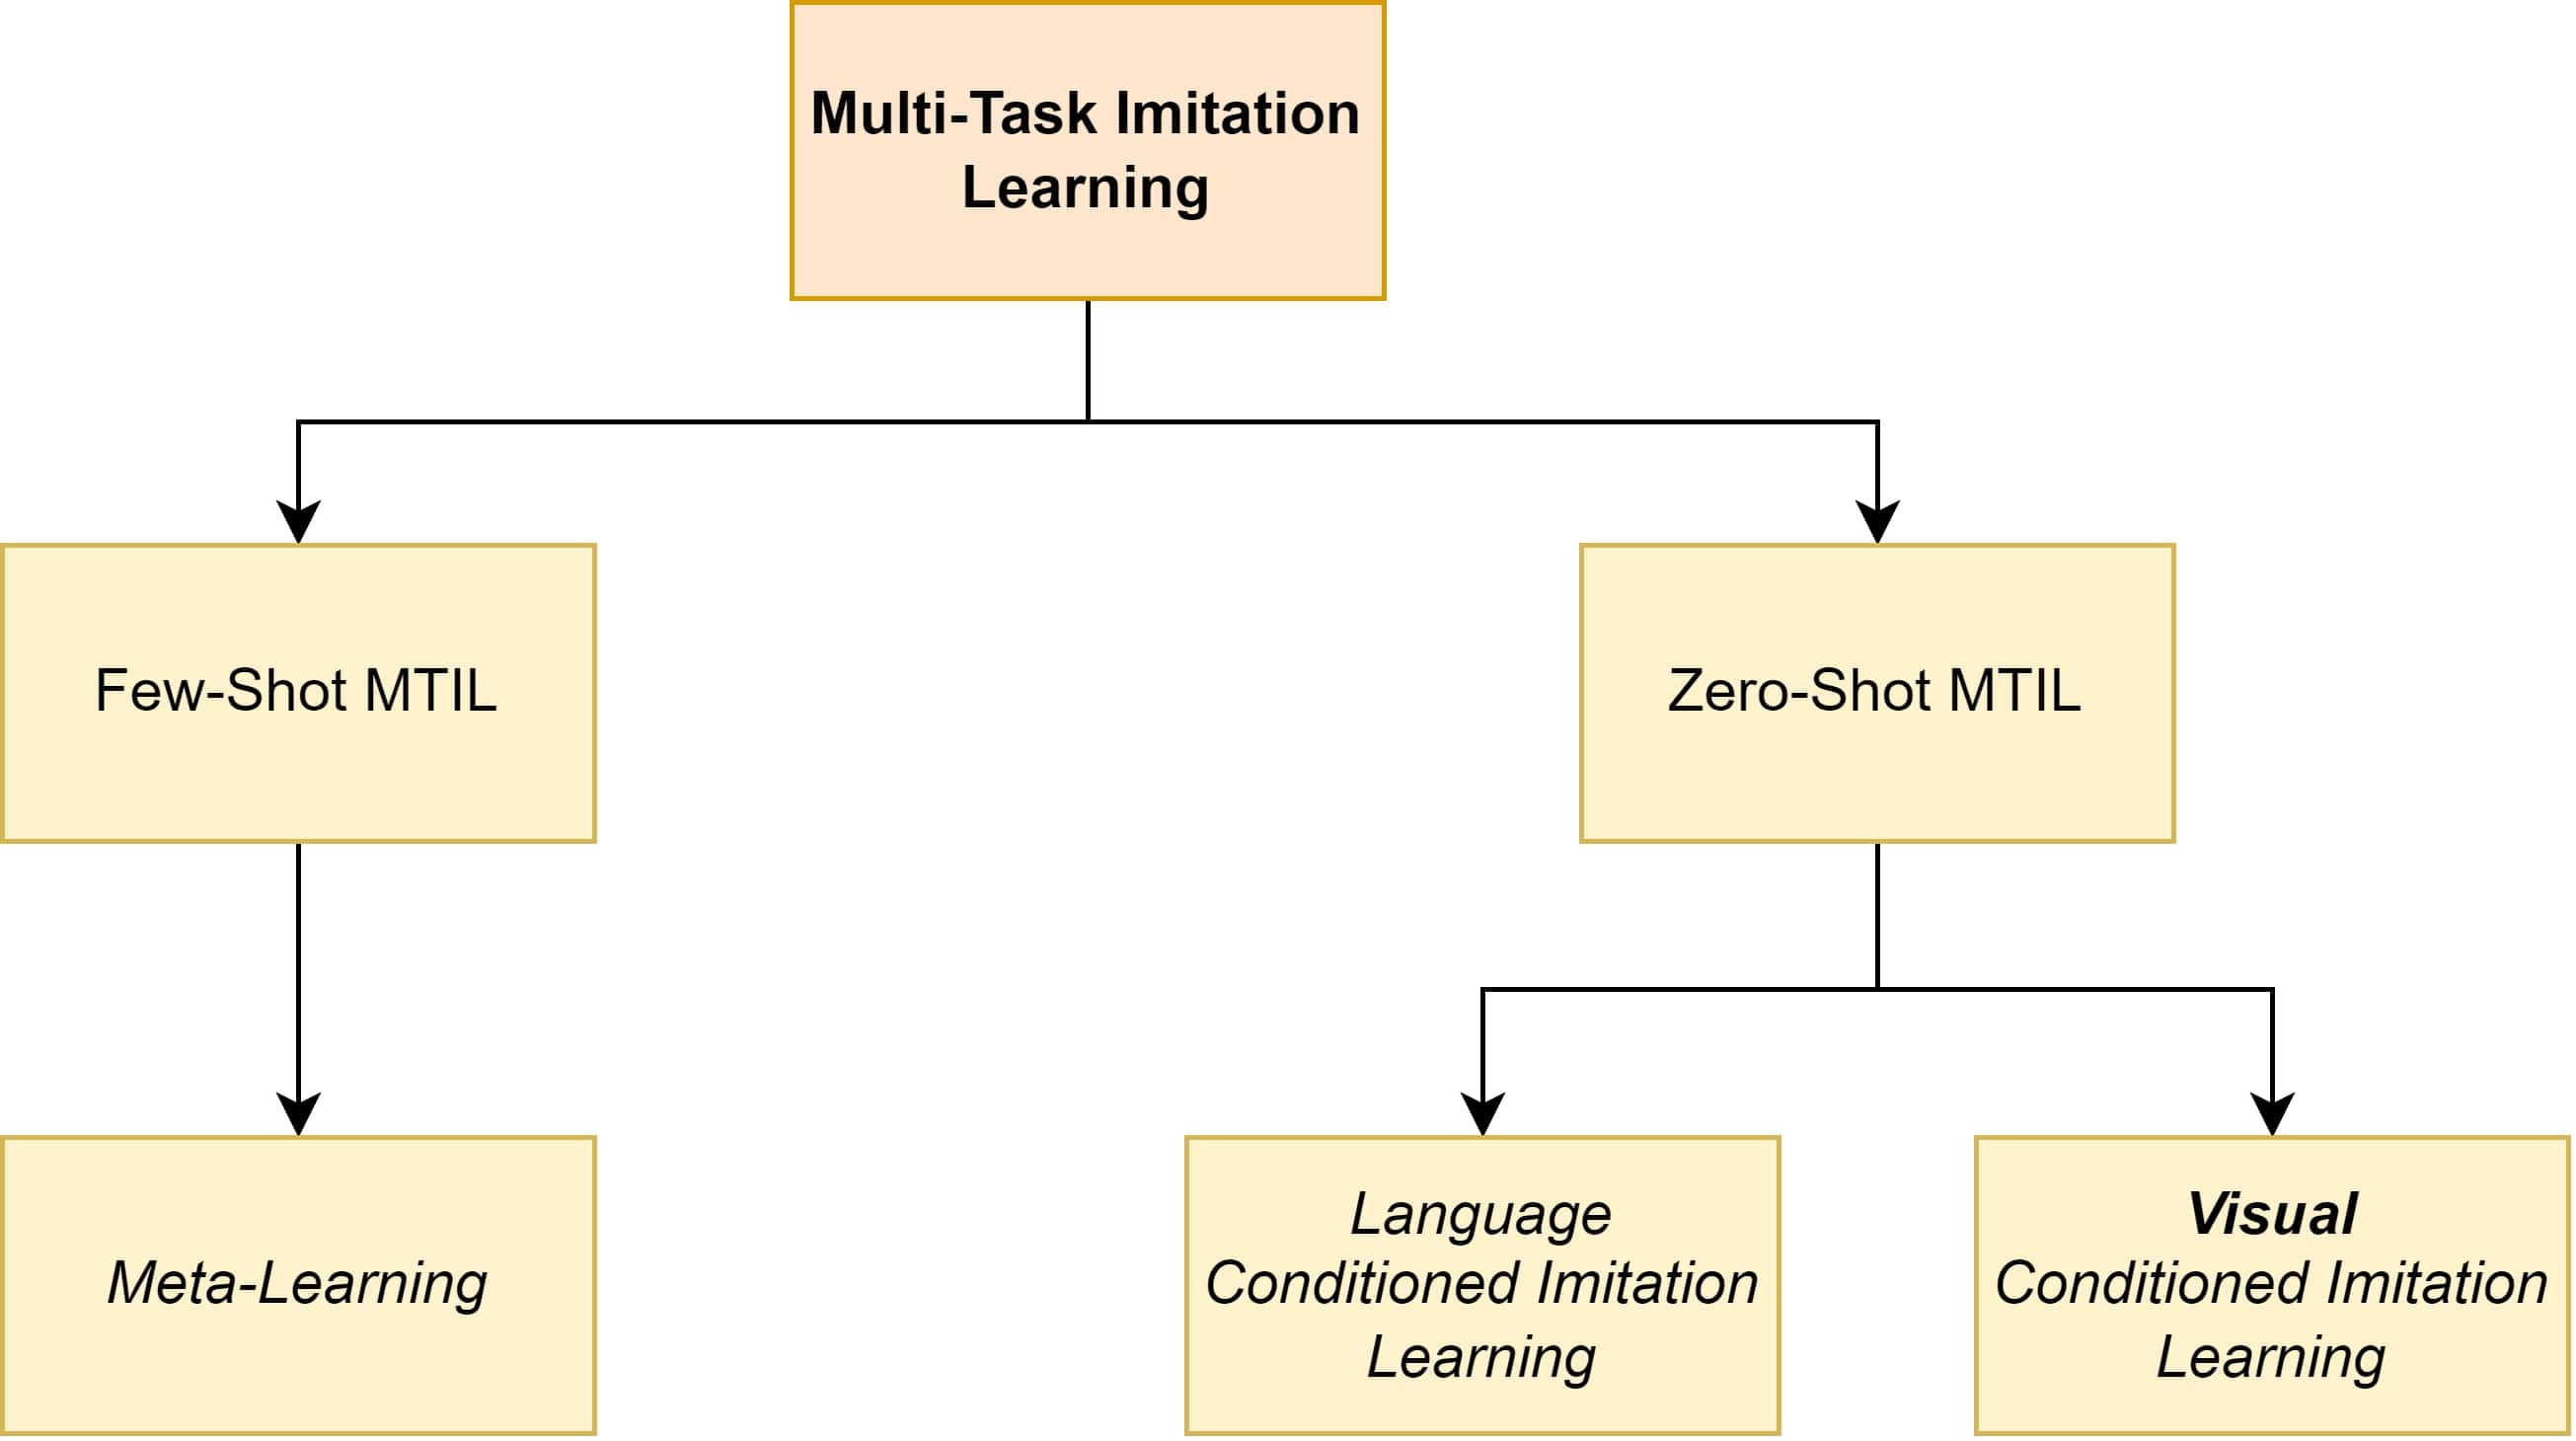
\includegraphics[width=0.8\textwidth]{figures/images/MTIL_taxonomy.jpg}
    \caption{Multi-Task Imitation Learning Taxonomy.}
    \label{fig:mtil_taxonomy}
    
\end{figure}


\textbf{Few-Shot MTIL} refers to approaches designed to train a model on a variety of tasks so that it can effectively solve a new task using only few samples and consequently requires only a few back-propagation steps \cite{finn2017maml}. In this context, one of the most significant learning paradigms, especially relevant to robotic manipulation, is \textit{Meta-Learning}. The goal of Meta-Learning is to train a model that can ``learn to learn," meaning it develops a set of general weights $\theta$ that, while not directly usable for solving any specific task within a distribution of tasks $\mathcal{T}$, can be quickly adapted through a few backpropagation steps to solve a given task within that distribution, $\mathcal{T}_{i} \in \mathcal{T}$. One of the most popular Meta-Learning algorithms is the \textit{Model-Agnostic Meta-Learning} (MAML) algorithm \cite{finn2017maml}, described in Algorithm \ref{alg:maml}. The MAML algorithm follows an iterative learning procedure consisting of two steps:
\begin{itemize}
    \item \textbf{Meta-Learning}: During this phase, task-specific weights $\theta_{i}$ are computed for each sampled task $\mathcal{T}_{i}$. Specifically, the \textit{meta-parameters} $\theta$ are updated according to the gradient obtained from evaluating the loss function on the $i^{th}$ task $\mathcal{T}_{i}$, where the function $f$ is parameterized by the meta-parameters $\theta$.

    \item \textbf{Meta-Adaptation}: In this phase, the meta-parameters are further refined. The loss function $f$, now parameterized by the task-specific parameters for the $i^{th}$ task, is used to adjust the meta-parameters based on the gradients derived from the sum of the loss functions evaluated on the task-specific weights. This process provides feedback to the meta-parameters $\theta$ from each task, leading to a generalized point that can be easily adapted to new tasks (Figure \ref{fig:maml_weights}).
\end{itemize}
\begin{algorithm}[t]
\caption{Model-Agnostic Meta-Learning (MAML) \cite{finn2017maml}}
\label{alg:maml}
\begin{algorithmic}
\REQUIRE Distribution over tasks $p(\mathcal{T})$
\STATE Randomly initialize $\theta$
\WHILE {$i=1, \dots N$}
    \STATE Sample batch of tasks $ \mathcal{T}_{i} \sim p(\mathcal{T})$
    \FOR {\textbf{all} $\mathcal{T}_{i}$}
        \STATE Evaluate $\nabla_\theta \mathcal{L}_{\mathcal{T}_{i}}(f_{\theta})$ w.r.t. $K$ examples
        \STATE Compute adapted parameters with gradient descent: $\theta'_{i} = \theta - \alpha \nabla_\theta\mathcal{L}_{\mathcal{T}_{i}}(f_{\theta})$
    \ENDFOR
    \STATE Update $\theta \leftarrow \theta - \beta \nabla_\theta \sum_{\mathcal{T}_{i} \sim p(\mathcal{T})} \mathcal{L}_{\mathcal{T}_{i}}(f_{\theta'_{i}})$
\ENDWHILE
\end{algorithmic}
\end{algorithm}
\begin{figure}[tb]
    \centering
    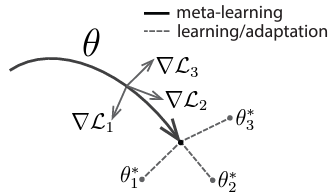
\includegraphics[width=0.6\textwidth]{figures/images/maml_weights.png}
    \caption{Diagram of MAML algorithm, which optimizes for a representation $\theta$ that can quickly adapt to new tasks}
    \label{fig:maml_weights}
\end{figure}

The MAML algorithm is the base for different methods which apply Few-Shot Imitation Learning in the context of Behavioral Cloning \cite{finn2017one_shot_visual_il,yu2018daml,yu2018one_shot_hil}.

In \cite{finn2017one_shot_visual_il}, MAML algorithm was used to prove the effectiveness of Meta-Learning in the context of real robot manipulation, with visual observations, as opposite to \cite{duan2017one_shot_il}. A Convolutional Neural Network was trained by following the Algorithm \ref{alg:maml}, using as loss-function the Mean Squared Error, computed between the predicted action and the ground truth one. For real-robot experiments a dataset of \textbf{1300} placing demonstrations (i.e., place an holded object in a target container), containing near to \textbf{100} different objects, was collected through teleportation. The trained system was tested by performing the adaptation step on one video demonstration, over 29 new objects, moreover, between the video demonstration and the actual execution, the objects configuration was changed. In this setting the system reached the $\mathbf{90\%}$ of success rate, outperforming baseline methods based on LSTM \cite{duan2017one_shot_il}, and contextual network (i.e., a Convolutional Neural Network that takes in input the current observation and the image representing the target state).

In \cite{yu2018daml}, the \textit{Domain Adaptive Meta-Learning} (DAML) algorithm was introduced to infer a policy from a single human demonstration. 
\newline It employs a two-step process. First, the \textbf{Meta-Learning step}, where for each task $\mathcal{T}$, human demonstrations $\mathcal{D}^{h}_{\mathcal{T}}$ and robot demonstrations $\mathcal{D}^{r}_{\mathcal{T}}$ (Figure \ref{fig:daml_tasks}) are used to learn the \textit{initial policy parameters} $\theta$ and the \textit{adaptive loss} parameters $\psi$, solving the problem in Formula \ref{eq:daml}.
\begin{equation}
 \label{eq:daml}
 \underset{\theta,\psi}{\min} \sum_{\mathcal{T} \sim p(\mathcal{T})} \sum_{\mathbf{d}^{h} \sim D^{h}_{\mathcal{T}}} \sum_{\mathbf{d}{^r} \sim D^{r}_{\mathcal{T}}} \mathcal{L}_{BC}(\theta - \alpha \nabla_\theta\mathcal{L}_{\psi}(\theta,\mathbf{d}^{h}), \mathbf{d}^{r})
\end{equation}

\newline The outer loss is the classic supervised Behavioral Cloning loss, defined as $\mathcal{L}_{BC}(\phi, \mathbf{d^{r}}) = \sum_{t} \log(\pi_{\phi}(a_{t} \mid s_{t}, o_{t}))$. The inner loss, $\mathcal{L}_{\psi}$, is a learned \textbf{adaptive loss}. Specifically, $\mathcal{L}_{\psi}$ is used during Meta-Adaptation, where the policy parameters are updated by evaluating the gradients derived from $\mathcal{L}_{\psi}$. This process involves a video of a human demonstrating a new task $\mathcal{T}$ as input, leading to the policy update defined by $\phi_{\mathcal{T}} = \theta - \alpha \nabla_{\theta} \mathcal{L}_{\psi}(\theta, \mathbf{d}^{h})$. 
\newline This adaptive loss is the key component proposed in DAML. To use it effectively, it is necessary to learn the parameters $\psi$, observing how there is no direct correspondence between the human video demonstration and the robot ground truth actions. To address this challenge, the authors of DAML observed that while the policy learns to produce appropriate actions through the $\mathcal{L}_{BC}$ loss, the adaptive loss should instead adjust the perceptual aspect of the policy, focusing on human motion and the manipulated object. Based on this insight, the authors implemented the function $\mathcal{L}_{\psi}$ using a 1D Temporal Convolutional Network (Figure \ref{fig:daml_temporal_adaptation_loss}). The convolutional layers are applied to a stack of embeddings generated by the policy $\pi$ across different frames of the video demonstrations. The parameters of this module are learned during the meta-training phase, following the weight update process described in Formula \ref{eq:daml_temporal_adaptation_loss}. The objective of $\mathcal{L}_{\psi}$ is to generate task-specific policy parameters $\phi_{\mathcal{T}}$ that guide the policy to produce effective actions.

\begin{equation}
 \label{eq:daml_temporal_adaptation_loss}
 \begin{matrix}
    (\theta, \psi) \leftarrow(\theta, \psi)-\beta \nabla_{\theta, \psi} \mathcal{L}_{\mathrm{BC}}\left(\phi_{\mathcal{T}}, \mathbf{d}^r\right) \\ \\
   \phi_{\mathcal{T}}=\theta-\alpha \nabla_\theta \mathcal{L}_\psi\left(\theta, \mathbf{d}^h\right)
   \end{matrix}
\end{equation}

\newline Experimental evaluation on tasks such as placing, pushing, and pick-and-place, has shown that: \begin{itemize}
    \item The system was able to generalize across both new objects and objects configuration starting from only a single human demonstration.
    \item A performance degradation was observed in large domain-shift experiments, such as novel backgrounds and different camera view-points.
\end{itemize}
\begin{figure}[t]
    \centering
    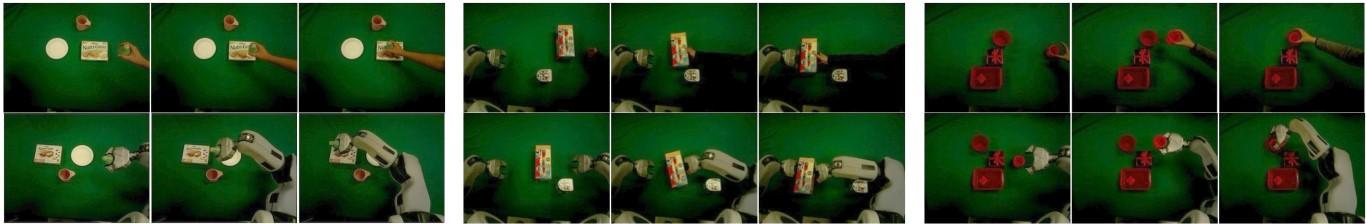
\includegraphics[width=\textwidth]{figures/images/daml/tasks.jpg}
    \caption{Tasks performed in \cite{yu2018daml}. (Top row) Human demonstration, (Bottom row) robot demonstration. (Left) Placing task, (Middle) pushing task, (Right) pick-and-place task.}
    \label{fig:daml_tasks}
\end{figure}

\begin{figure}[t]
    \centering
    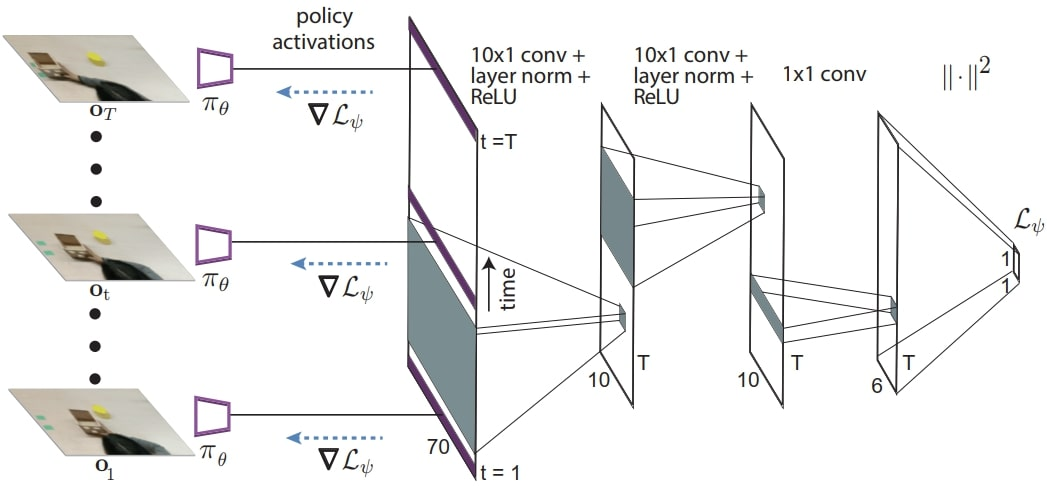
\includegraphics[width=0.8\textwidth]{figures/images/daml/daml_temporal_adaptation_loss.jpg}
    \caption{The Temporal Adaptation Loss architecture applies 1D temporal convolutional layers to the stacked embeddings generated by the policy $\pi$ from the frames of the human video demonstration.}
    \label{fig:daml_temporal_adaptation_loss}
\end{figure}

Meta-Learning algorithms have demonstrated interesting properties, notably their capacity for few-shot generalization to novel objects and object configurations. However, it has been observed that during the adaptation step, these methods tend to loose their effectiveness in performing other tasks. This limitation has underscored the need for the development of Multi-Task Imitation Learning methods, which aim to address these shortcomings and enable more versatile task execution in complex scenarios. These kinds of methods will be discussed in the following paragraphs.

\textbf{Zero-Shot MTIL} refers to approaches that aim to train a model capable of solving different tasks without any further adaptation or backpropagation steps. This approach addresses a key issue in Meta-Learning methods, which is the problem of forgetting how to solve previous tasks after adapting to a new one. The goal is to develop a single policy that can handle multiple tasks in a zero-shot manner.

In this context, a crucial design choice is how to convey the desired task to the policy. The literature identifies two main methods to address this problem:

\begin{enumerate}
    \item \textit{Language Conditioned}: These methods leverage natural language descriptions of tasks to inform the model about the task to be executed.
    \item \textit{Visual Conditioned}: These methods use visual information (e.g., goal-state images, video demonstrations) to provide the model with the task instructions.
\end{enumerate}

\textit{Language Conditioned}. As said a possible and intuitive way to inform the policy about which task to execute is through natural language description. Indeed, by looking to the phrase ``Pick the blue cube and place it in the red bow'', there are both information about the action to perform (pick and place) and which are the objects involved (blue cube and red bow). Consequently, by training a neural network on a diverse set of tasks, the system is expected to generalize its understanding to unseen objects within familiar tasks and entirely novel tasks composed of fundamental actions learned during training. This approach highlights the potential for \textbf{robust} and \textbf{adaptable} \textbf{human-robot interaction} in real-world scenarios.

Foundational research, such as that by \cite{stepputtis2020language} and \cite{jang2022bc_z}, has sought to explore the previously mentioned hypothesis. Notably, \cite{stepputtis2020language} introduced an innovative architectural framework, depicted in Figure \ref{fig:language_conditioned}, marking the first instance of seamlessly integrating language, vision, and control tasks. This model is composed of two critical components: a \textit{Semantic Model}, which generates a task embedding denoted as $e$ by processing the initial scene image and the accompanying text command, and a \textit{Control Model}, which generates the control signal using the current robot state $r_{t}$ and the task embedding $e$.

A crucial aspect of such architectures is the management of the visual state, represented by the image $I$, and the command $v$, to create a meaningful embedding $e$ that encapsulates both the current scene state and the desired command. Specifically, the image is first processed using a pre-trained object detection network (Faster R-CNN \cite{fastrcnn}) to identify salient objects in the robot's environment. The detected objects are represented by feature vectors, which include class and bounding box information. Concurrently, the language command is embedded into a suitable representation using a language embedding technique (e.g., GloVe \cite{pennington2014glove}), with the command vector $V$ encoded by a recurrent GRU unit. To associate the objects identified with the sentence embedding $s$, a likelihood value is computed for each object proposal $a_{i} = w_{a}^{T} f_{a}([\text{f}_{i}, s])$, and a probability distribution is computed over the candidates $\mathbf{a} = \text{softmax}([a_0, \dots, a_c])$. Finally, the task embedding $e$ is formed by a fully connected layer that takes as input the sentence embedding $s$ and the weighted sum of object candidate features $e'= \sum_{i=0}^{c} f_{i}a_{i}$.

Training of this model was conducted on two fundamental tasks, namely ``Picking" and ``Pouring", within scenarios featuring multiple objects of the same category, which served as distractors (see Figure \ref{fig:objects}). The subsequent testing experiments demonstrated the system's capability to successfully complete the picking task 98 out of 100 times and the pouring task 85 out of 100 times within novel scenarios. These results serve as compelling evidence of the efficacy and potential of language-conditioned methodologies in the field.
\begin{figure}[t]
    \centering
    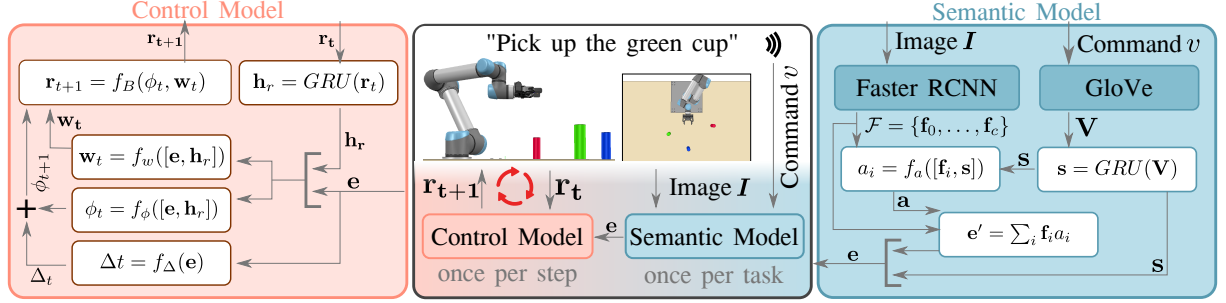
\includegraphics[width=0.9\textwidth]{figures/images/language_conditioned/architecture.png}
    \caption{Architecture proposed in \cite{stepputtis2020language}. The \textit{Semantic Model} takes in input the image $I$ and the command $v$, generating a command conditioned embedding $e$. The \textit{Control Module} receives in input the embedding $e$ and the current robot state $r_{t}$ and produces the next control signal.}
    \label{fig:language_conditioned}
\end{figure}

\begin{figure}[t]
    \centering
    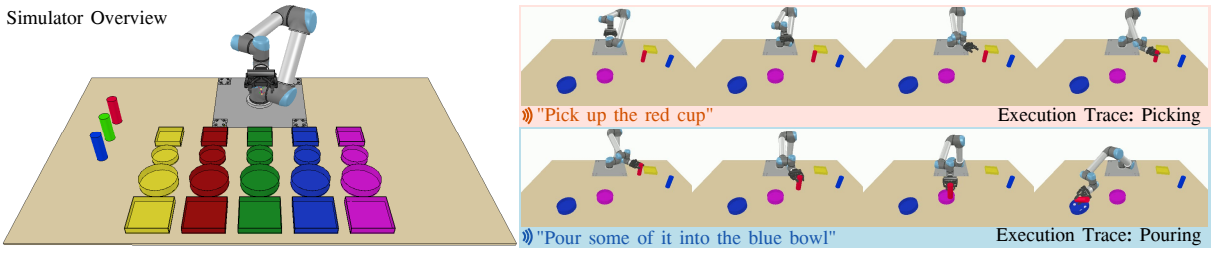
\includegraphics[width=0.9\textwidth]{figures/images/language_conditioned/objects.png}
    \caption{(Left) Set of object used in \cite{stepputtis2020language}. (Right) Sample of task execution (right)}
    \label{fig:objects}
\end{figure}


In \cite{jang2022bc_z}, the authors take a step toward developing a more general agent by proposing a large-scale dataset comprising \textbf{100} diverse manipulation tasks. The demonstrations were collected through both expert teleoperation and a shared autonomy process (HG-DAgger \cite{kelly2019hg_dagger}). The skills covered included pick-and-place, grasp, pick-and-drag, pick-and-wipe, and push skills. The dataset was used to train the network shown in Figure \ref{fig:bcz_architecture}. Notably, the samples consisted of the current robot observation, with conditioning provided by either a \textit{\textbf{natural language description}} or a \textit{\textbf{human video demonstration}}.

The goal was to train a conditioned policy using the current observation $o_{t}$ and a task representation $c$, enabling the policy to generalize to new tasks in a zero-shot manner (i.e., without fine-tuning). In contrast to previous methods, this approach does not rely on pre-trained object detectors for identifying candidate regions. Instead, the Task Embedding is directly injected into the Feature Maps generated by the Convolutional Neural Network (ResNet-18), facilitated through the FiLM layer \cite{perez2018film}.

Experimental results shown that, over 28 held-out tasks, containing both completely new objects, and known objects but in different tasks, an average success rate of \textbf{38\%} was reached in the easiest setting, with only one distractor and with natural language instruction. The success rate dropped to \textbf{4\%} in the hardest setting with 4 distractors and video conditioning.
\begin{figure}[t]
    \centering
    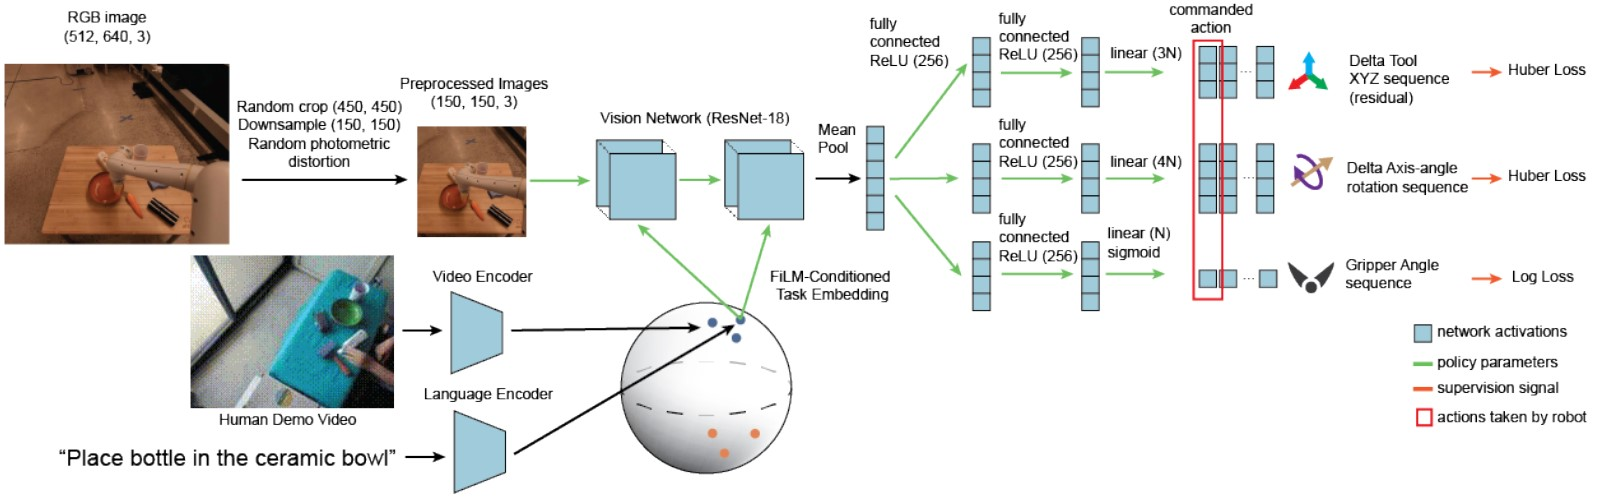
\includegraphics[width=0.9\textwidth]{figures/images/bc_z/bc-z-network.jpg}
    \caption{Architecture proposed in \cite{jang2022bc_z}. Here, the Task Embedding is injected directly in the Feature Maps generated by the ResNet-18.}
    \label{fig:bcz_architecture}
\end{figure}


Foundational research in the field of Language-Conditioned Multi-Task Imitation Learning has demonstrated promising results in zero-shot generalization. However, the robustness of their performance remains a challenge. Subsequent research, as highlighted in \cite{brohan2022rt,mees2022calvin,mees2022hulc}, has focused on enhancing performance. 

In particular, the authors of \cite{brohan2022rt} sought to investigate whether the transfer of knowledge from extensive, diverse, and task-agnostic datasets, which has enabled modern machine learning models to excel in zero or few-shot learning scenarios for new and specific tasks, is applicable within the realm of robotics. This inquiry arises due to the presence of high-capacity architectures capable of assimilating knowledge from such large datasets. To explore this prospect, the authors in \cite{brohan2022rt} introduced a comprehensive dataset comprising over 130,000 demonstrations collected across more than 700 household tasks (Figure \ref{fig:rt_1_dataset}). Additionally, they proposed a Language-Conditioned Transformer-based architecture (Figure \ref{fig:rt_1_model}). Here the authors made relevant modification in the architecture, with respect to the previous BC-Z architecture \cite{jang2022bc_z}.Indeed, they modified the Visual Module by using an EfficientNet \cite{tan2019efficientnet} instead of the ResNet-18. The instruction was encoded using the Universal Sentence Encoder \cite{cer2018universal}, and the policy was implemented through a Transformer. Additionally, the authors addressed the real-time constraints of robot control. To accelerate inference time and achieve a frequency of $3$ Hz, the authors employed a TokenLearner module \cite{ryoo2021tokenlearner}, which utilizes an attention mechanism to select the most relevant tokens, thereby reducing the number of tokens that the underlying control module must process to infer the action.
\begin{figure}[t]
    \centering
    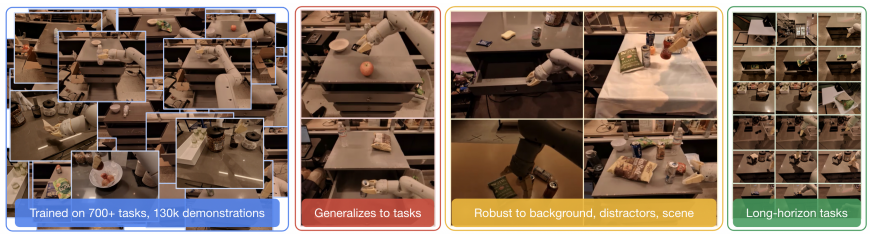
\includegraphics[width=0.8\textwidth]{figures/images/rt_1/dataset_image.png}
    \caption{Examples of household scenarios in RT-1 large-scale dataset.}
    \label{fig:rt_1_dataset}
\end{figure}

\begin{figure}[t]
    \centering
    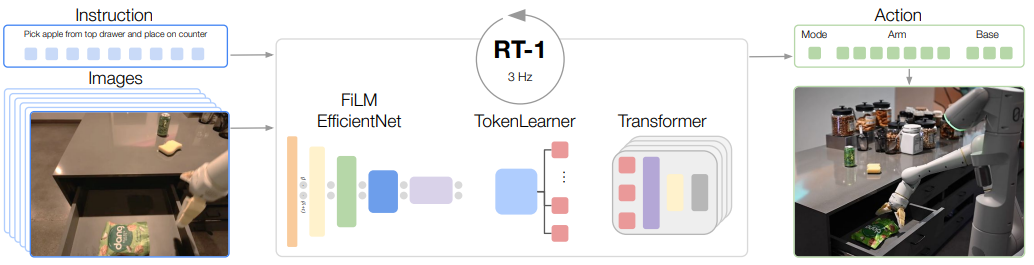
\includegraphics[width=\textwidth]{figures/images/rt_1/model.png}
    \caption{RT-1 Language-Conditioned Transformer based architecture proposed in \cite{brohan2022rt}.}
    \label{fig:rt_1_model}
\end{figure}
% \usepackage{graphicx}
% \usepackage{hhline}


\begin{table}
    \centering
    \caption{Distribution of tasks in large-scale dataset proposed in \cite{brohan2022rt}}
    \label{table:rf1_dataset}
    \resizebox{\linewidth}{!}{%
    \begin{tabular}{|c|c|c|c|} 
    \hline
    \textbf{Skill} & \textbf{Count} & \textbf{Description} & \textbf{Example Instruction} \\ 
    \hhline{|====|}
    Pick Object & 130 & Lift the object off the surface & pick iced tea can \\ 
    \hline
    Move Object Near Object & 337 & Move the first object near the second & move pepsi can near rxbar blueberry \\ 
    \hline
    Place Object Upright & 8 & Place an elongated object upright & place water bottle upright~ ~ \\ 
    \hline
    Knock Object Over & 8 & Knock an elongated object over & knock redbull can over \\ 
    \hline
    Open Drawer & 3 & Open any of the cabinet drawers & open the top drawer \\ 
    \hline
    Close Drawer & 3 & Close any of the cabinet drawers & close the middle drawer \\ 
    \hline
    Place Object into Receptacle & 84 & Place an object into a receptacle & place brown chip bag into white bowl \\ 
    \hline
    \begin{tabular}[c]{@{}c@{}}Pick Object from Receptacle\\and Place on the Counter\end{tabular} & 162 & \begin{tabular}[c]{@{}c@{}}Pick an object up from a location \\and then place it on the counter\end{tabular} & \begin{tabular}[c]{@{}c@{}}pick green jalapeno chip bag from\\~paper~bowl and place on counter\end{tabular} \\ 
    \hline
     & 9 & Skills trained for realistic, long instructions & \begin{tabular}[c]{@{}c@{}}open the large glass jar of pistachios \\~pull napkin out of dispenser grab scooper\end{tabular} \\ 
    \hhline{|====|}
    \textbf{Total} & 744 &  &  \\
    \hline
    \end{tabular}
    }
    \end{table}

It is worth noting the intriguing findings presented in Table \ref{table:rt1_results}. The model demonstrates robustness in performing tasks it has encountered previously and even achieves reasonable performance on tasks it has never seen before. However, a noticeable decline in performance occurs when the model faces novel backgrounds or scenarios with distracting objects, particularly when data for these situations is sparse. This trend is significant because, unlike domains such as Computer Vision and Natural Language Processing, where large-scale datasets can be easily obtained, collecting real-world robotic datasets is a labor-intensive and time-consuming process. Moreover, these datasets often have limited applicability to other research due to \textbf{disparities in action space, robot morphology, and scene representation}, as highlighted by \cite{brohan2022rt}. Therefore, the goal is to create a system capable of replicating tasks with minimal demonstrations, specifically gathered from the particular robot in use.

Furthermore, the decline in success performance when faced with distractor objects emphasizes that addressing the policy-learning problem in an end-to-end manner, which involves mapping high-dimensional and high-level inputs like images and text directly to low-dimensional, low-level outputs such as the actions to be executed, may not be the most effective approach. This is because such models might lack the necessary perceptual components that enable them to initially recognize the target object within the scene, subsequently navigate towards it, and commence the manipulation process. This process aligns with how humans approach manipulation tasks \cite{grill2003neural}.
% \usepackage{graphicx}
% \usepackage{hhline}


\begin{table}
    \centering
    \caption{Results reported in \cite{brohan2022rt} by training the same model RT-1 with different dataset size.}
    \label{table:rt1_results}
    \resizebox{\linewidth}{!}{%
    \begin{tabular}{|c|c|c|c|c|c|c|c|} 
    \cline{5-8}
    \multicolumn{1}{c}{} & \multicolumn{1}{c}{} & \multicolumn{1}{c}{} &  & \multicolumn{4}{c|}{Generalization} \\ 
    \hline
    Models & \% Tasks & \% Data & Seen Tasks & All & Unseen Tasks & Distractors & Backgrounds \\ 
    \hhline{|========|}
    RT-1 & 100 & \textbf{100} & 97 & 73 & 76 & \textbf{83} & 59 \\ 
    \hline
    RT-1 & 100 & \textbf{51} & 71 & 50 & 52 & \textbf{39} & 59 \\ 
    \hline
    RT-1 & 100 & \textbf{37} & 55 & 46 & 57 & \textbf{35} & 47 \\ 
    \hline
    RT-1 & 100 & \textbf{22} & 59 & 29 & 14 & \textbf{31} & 41 \\
    \hline
    \end{tabular}
    }
    \end{table}

As we have seen up to now, all the proposed methods were tested on different robotic platforms with different scenarios and environments. As in other Computer Vision problem, there are no well known benchmark that are used by the researchers around the world. To solve this problem, authors in \cite{mees2022calvin} proposed CALVIN (Composing Actions from Language and Vision), which is an open-source simulated benchmark designed for learning long-horizon language-conditioned tasks in robotic manipulation. Specifically, CALVIN proposes a set of 34 manipulation tasks in 4 different environments (Figure \ref{fig:calvin_env}). 
\begin{figure}[t]
    \centering
    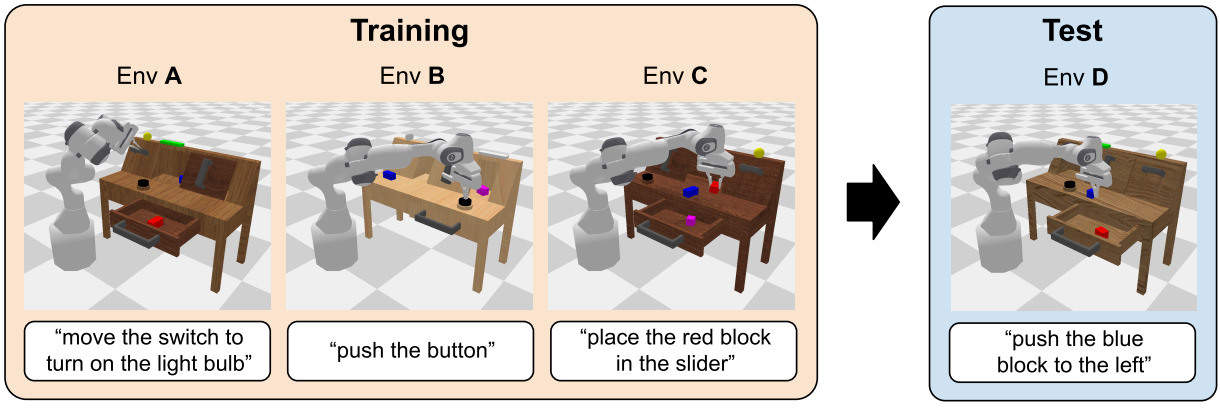
\includegraphics[width=0.9\textwidth]{figures/images/calvin/calvin_env.jpg}
    \caption{Environment proposed in CALVIN benchmark \cite{calvin}. The environments have different textures and all static elements such as the sliding door, the drawer, the light button, and switch are positioned differently}
    \label{fig:calvin_env}
\end{figure}

This benchmark was used by \cite{mees2022hulc,mees2023hulc++,reuss2024multimodal}. Specifically, the work proposed in \cite{reuss2024multimodal} is actually the best performing method on the CALVIN benchmark. The authors proposed an architecture that is able to handle goals described in terms of both natural language description and goal image, moreover they used a Diffusion Transformer Model as policy (Figure \ref{fig:mdt_architecture}). To reach this goal, the authors had to solve first the problem related to how to force the Multimodal Transformer Encoder to generate the same behavior independently of the goal modality. To solve this problem authors of MDT proposed two auxiliary self-supervised loss functions:
\begin{itemize}
    \item \textit{Masked Generative Foresight} (MGF) is a reconstruction loss function designed to ensure that the MDT generates embeddings that guide robot behavior consistently across different modalities. This means that the tokens generated by the MDT can be used to construct image patches representing feature states, whether the goal is described in terms of an image or a language description. Specifically, given the latent embedding of the MDT encoder for state $s_i$ and goal $g$, MGF trains a Vision Transformer (ViT) to reconstruct a sequence of 2D image patches $(u_1, \dots, u_U) = \text{patch}(s_{i+v})$ corresponding to the future state $s_{i+v}$.
    \item \textit{Contrastive Latent Alignment} (CLA) is a contrastive loss term designed to encourage the MDT to align the embeddings generated from a goal image with those generated from a language description. For each training sample $(s_i, a_i)$ paired with a multimodal goal specification $G_{s_i,a_i} = \{o_i, l_i\}$, CLA reduces the image and language goals to vectors $z_i^o$ and $z_i^l$, respectively. The CLA loss is then computed using the InfoNCE loss, based on the cosine similarity $C(z_i^o, z_i^l)$ between the image-goal conditioned state embedding $z_i^o$ and the language-goal conditioned state embedding $z_i^l$.
\end{itemize}
\begin{figure}[t]
    \centering
    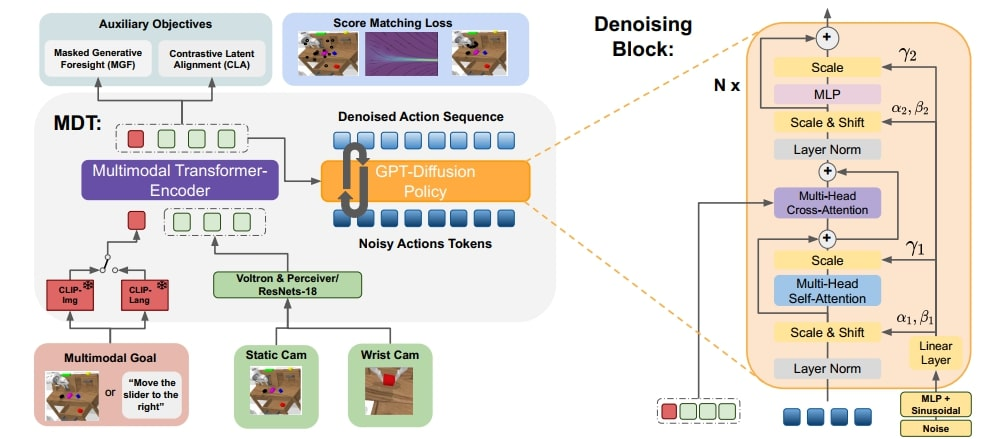
\includegraphics[width=\textwidth]{figures/images/mdt/mdt_architecture.jpg}
    \caption{The Multimodal Diffusion Transformer (MDT) architecture proposed in \cite{reuss2024multimodal}}
    \label{fig:mdt_architecture}
\end{figure}
As mentioned, this method was tested on the CALVIN benchmark, specifically in the $ABCD \rightarrow D$ test scenario, where the model was trained on the $ABCD$ environments and tested on environment $D$. The CALVIN benchmark comprises a set of 1000 rollouts, with each rollout consisting of a sequence of 5 commands. It is noteworthy that the MDT architecture successfully completed $80\%$ of the rollouts up to the fifth command. In particular, the MGF loss was observed to have a significant impact on system performance, improving the success rate for the fifth command from $69.8\%$ to $79.4\%$. This demonstrates that making the embedding informative about the system's evolution can meaningfully guide the diffusion system, which predicts actions over a certain time horizon into the future.

In the context of Language Conditioned MTIL, other important works to cite include \cite{shridhar2022cliport, shridhar2023perceiver}. Specifically, the authors in \cite{shridhar2022cliport} introduced CLIP-Port, a two-stream architecture that explicitly models the two key tasks in language-conditioned imitation learning: reasoning about \textbf{what to do} and reasoning about \textbf{how to do it}. The former task, referred to as \textit{semantic reasoning}, is derived from the text-based command and is handled using a pre-trained CLIP architecture \cite{radford2021learning}. The latter task, known as \textit{spatial reasoning}, is managed by leveraging the Transporter architecture \cite{zeng2021transporter}. The overall architecture (Figure \ref{fig:clip_port_architecture}) is an Encoder-Decoder framework that ultimately outputs an \textbf{affordance map}, which identifies the locations for executing pick or place operations (Figure \ref{fig:clip_port_affordance}).

During testing, this method was not directly compared with other Language Conditioned MTIL approaches. However, the results obtained allow for several observations. Notably, for tabletop manipulation tasks, the ability to reason using both spatial and semantic features enables a high success rate (ranging from $80\%$ to $90\%$) on tasks involving seen object attributes, such as color, even with a relatively low number of demonstrations (100). However, similar to the results reported in Table \ref{table:rt1_results}, CLIP-Port also struggles with entirely novel tasks, as evidenced by a significant drop in performance when dealing with unseen object attributes and a lower number of demonstrations.

\begin{figure}[t]
    \centering
    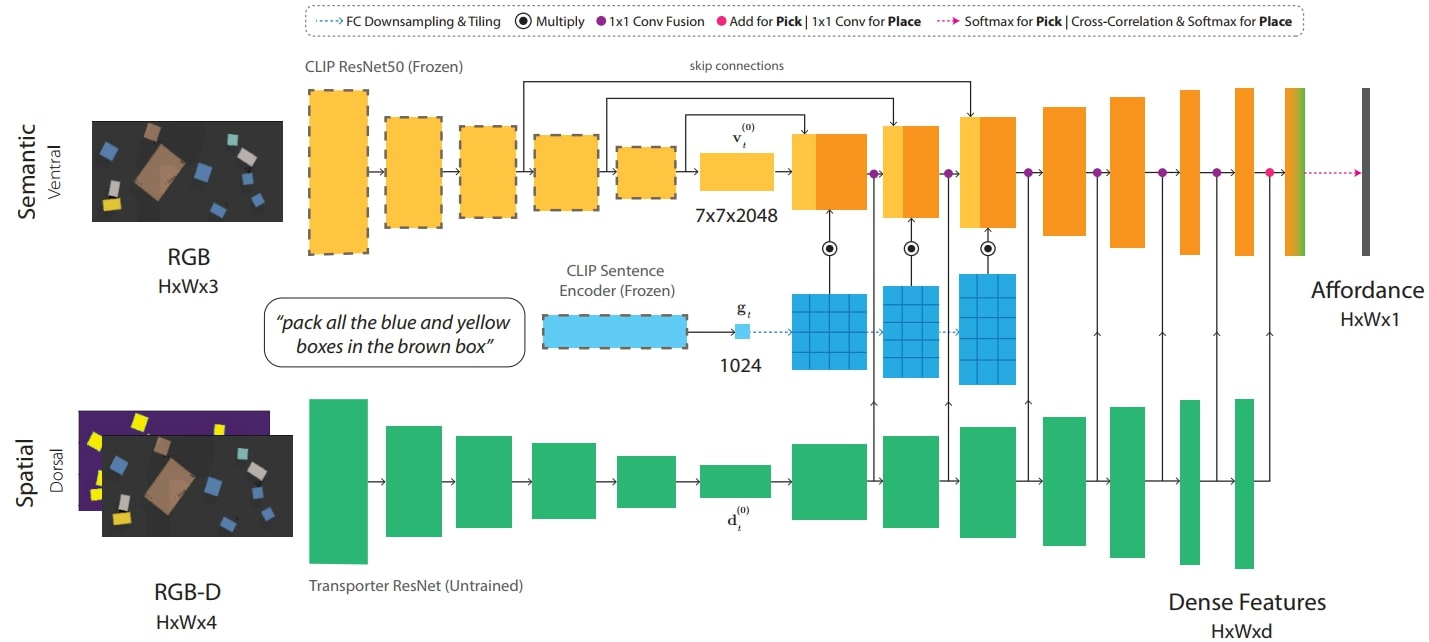
\includegraphics[width=\textwidth]{figures/images/clip_port/architecture.jpg}
    \caption{The Dual Stream architecture proposed in \cite{shridhar2022cliport} consists of two parallel streams: a semantic stream and a spatial stream. The semantic stream utilizes a frozen CLIP ResNet50 to encode the RGB input, with the decoder layers conditioned by tiled language features from the CLIP sentence encoder. Meanwhile, the spatial stream encodes the RGB-D input, and its decoder layers are laterally fused with those of the semantic stream. The final output is a map of dense pixelwise features, which is used to predict pick or place affordances.}
    \label{fig:clip_port_architecture}
\end{figure}

\begin{figure}[t]
    \centering
    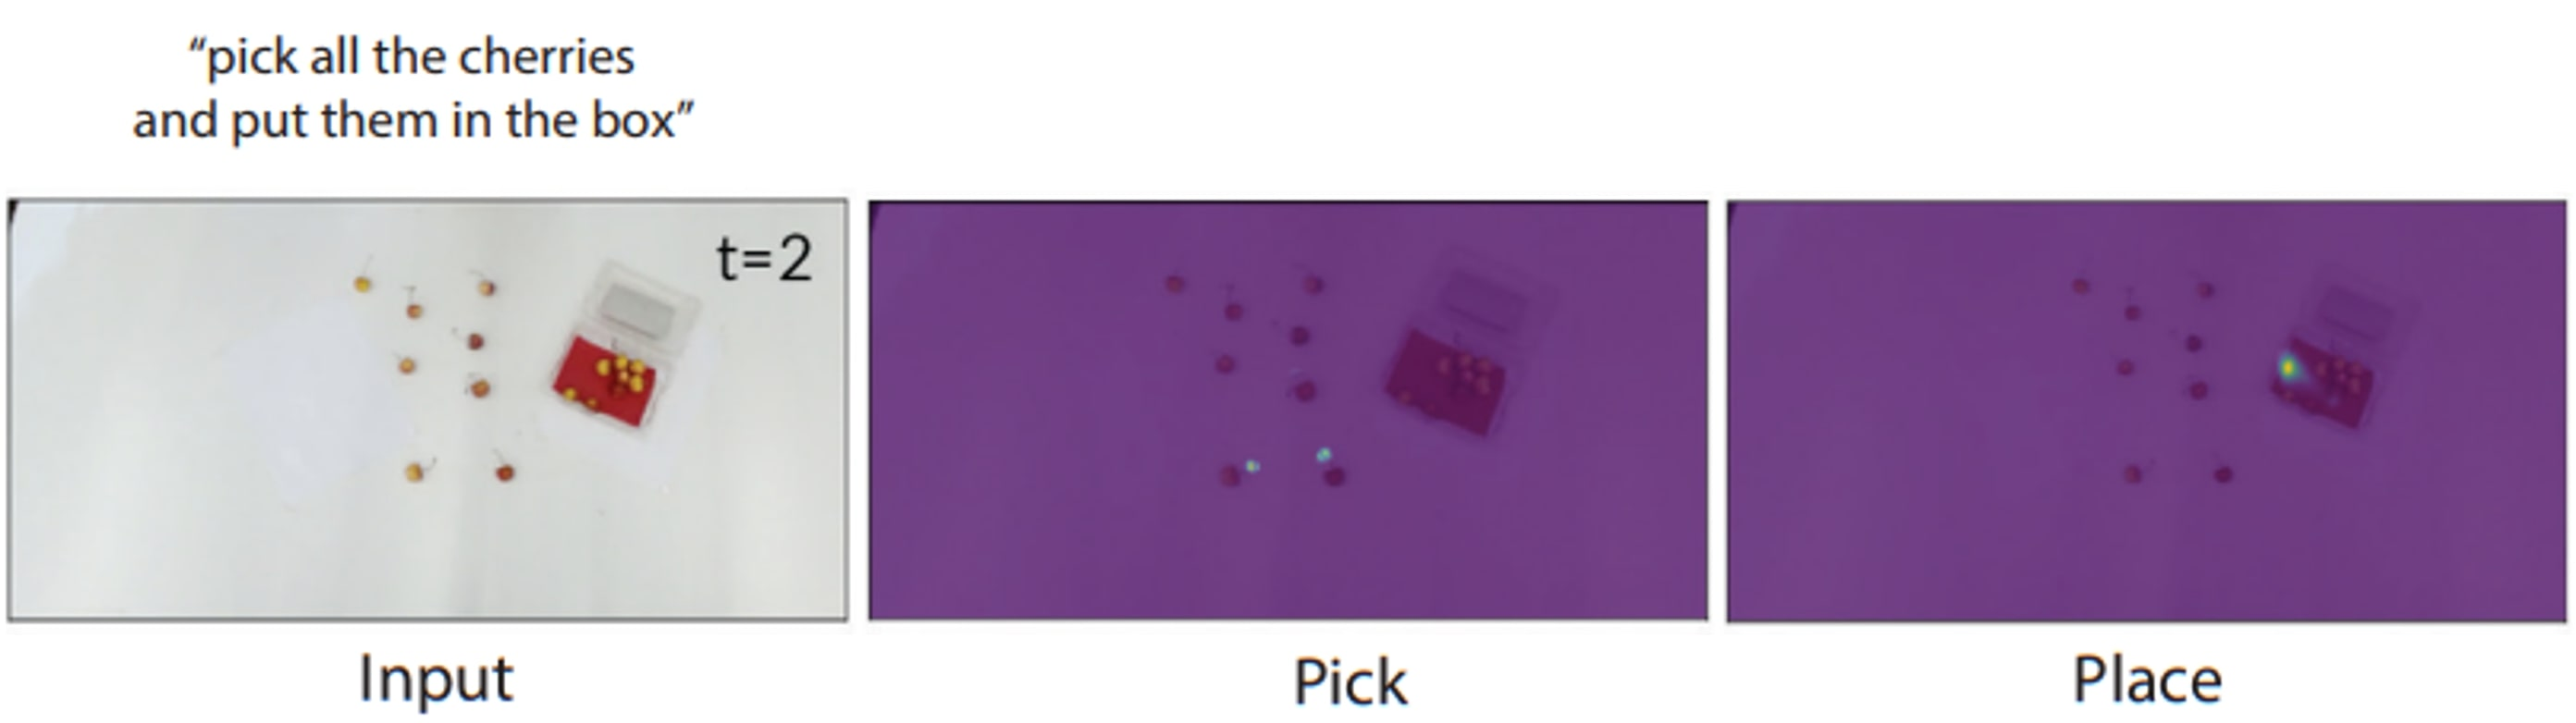
\includegraphics[width=0.8\textwidth]{figures/images/clip_port/affordance_map.jpg}
    \caption{Example of affordance map. (Left) The top-view input image. (Center) The affordance map for the pick-operation, since the task is to grab cherries the map highlights the two pickable cherries. (Right) The affordance map for the place operation.}
    \label{fig:clip_port_affordance}
\end{figure}

In conclusion, as discussed in this paragraph, considerable research effort has been dedicated to addressing the problem of Language Conditioned MTIL, particularly in terms of architectural designs and learning strategies. However, it remains challenging to draw definitive conclusions from these various approaches, as they are generally not evaluated on a common benchmark. Despite this issue, some trends can be observed. There is clearly room for improvement in the generalization capabilities of these methods, particularly in handling novel scenarios and tasks. Additionally, data efficiency remains a concern, as there is a noticeable decline in performance as the number of expert trajectories decreases. Another challenge is the ability to manage cluttered scenes with \textbf{relevant distractors}, objects that may have been manipulated during training but must be ignored in the target task, which can lead to occlusion and/or confusion.

\textit{Visual Conditioned} refers to methods that use visual information as a conditional signal. This information can be represented either as an image depicting the desired goal state or as a sequence of frames illustrating how the task should be performed. The idea behind this kind of methods is to build systems that are able to replicate tasks by observing the execution performed by other agents, like human can learn task by mimicking the execution of other humans.

Preliminary works, such as those by \cite{james2018task_embedded} and \cite{bhutani2022attentive_one_shot}, introduced architectures conditioned on the first and last frames of task demonstrations. Specifically, in \cite{james2018task_embedded}, the authors proposed TecNets (Task-Embedded Control Networks), an architecture illustrated in Figure \ref{fig:task_embedded}. TecNets consist of two main components:

\begin{itemize}
    \item \textit{Task-Embedding Network}: The purpose of this network is to create an embedding space where demonstrations of the same task are closely clustered, while embeddings of different tasks are kept as distant as possible. This network is trained using a contrastive loss function, defined in Formula \ref{eq:task_loss}, which ensures that the embedding of the $k^{th}$ sample of the $j^{th}$ task is similar to the "sentence" representing that task (i.e., the average of the embeddings of the $j^{th}$ task) and maximizes the distance from the sentences of other tasks.
    \begin{equation}
        \label{eq:task_loss}
        \mathcal{L}_{emb} = \sum_{\tau^{j}_{k} \in \mathcal{T}^{j}}\sum_{ \mathcal{T}^{i} \notin \mathcal{T}^{j}} \max \left[ 0, \text{margin} - s^{j}_{k}\cdot s^j + s^{j}_{k}\cdot s^i \right]
    \end{equation}
    \item \textit{Control Network}: This module implements the policy $\pi$, which takes as input the current observation $o$ and the sentence $s$ of the desired task. It then generates the corresponding action for the robot, conditioned on the task.
\end{itemize}

\begin{figure}[t]
    \centering
    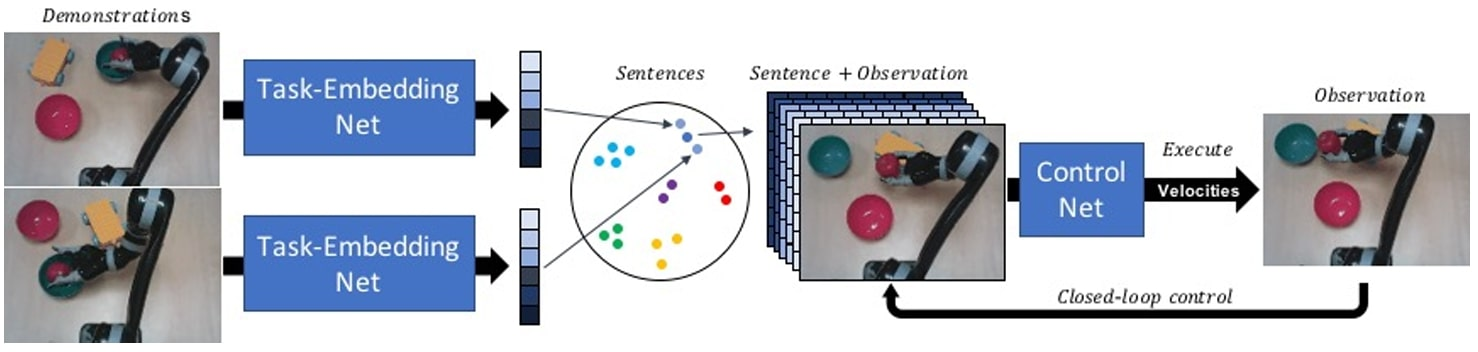
\includegraphics[width=\textwidth]{figures/images/task_embedded/task_embedded.jpg}
    \caption{Architecture proposed in \cite{james2018task_embedded}. The \textit{Task Embedding Net} generates the embedding representing the task to be performed given the goal image. The \textit{Control Net} implements the policy, and takes in input the current observation and the tiled task embedding.}
    \label{fig:task_embedded}
\end{figure}


The results from this preliminary work demonstrated the feasibility of training a vision-conditioned system capable of solving tasks in a zero-shot manner. The system achieved a success rate of \textbf{86.31}\% on a simulated 2D reaching task and \textbf{77.25}\% on a simulated pushing task. However, it is important to note a significant limitation of these approaches: the conditioning signal often fails to adequately capture critical information about the optimal strategy for solving the task. This shortcoming arises because the conditioning signal does not fully encode the strategies needed for effective task execution.


The methodologies introduced in \cite{dasari2021transformers_one_shot} and \cite{mandi2022towards_more_generalizable_one_shot} aim to advance the concept of an ideal multi-task agent, capable of replicating new tasks based on a single demonstration, often performed by another agent (e.g., a robot or a human).

In \cite{dasari2021transformers_one_shot}, the authors focused on training a vision-based control architecture (depicted in Figure \ref{fig:tosil_architecture}) that can replicate a task demonstrated through a set of frames sampled from a video of another agent performing the task. The architecture relies on two main components:
\begin{itemize}
    \item \textit{ResNet-18} \cite{resnet}, which serves as the backbone for extracting visual embeddings from the current agent state and the demonstration frames.
    \item \textit{Transformer} \cite{vaswani2017attention}, which uses the attention mechanism to combine embeddings from the demonstration frames with the current visual observation.
\end{itemize}

This architecture was trained using multiple loss terms, specifically:
\begin{itemize}
    \item \textit{Behavioral Cloning} term $\mathcal{L}_{BC}$ (Formula \ref{eq:tosil_bc}), a supervised loss function used to learn the action to perform given the agent's observation and the demonstrated task. Specifically, the loss function is a negative log-likelihood, computed over a mixture of learned logistic distributions, where the $i^th$ component is parameterized according to the mean and variance $(\mu_{i}, \sigma_{i})$ which are estimated through a MLPs.
    \begin{equation}
        \label{eq:tosil_bc}
        \mathcal{L}_{BC} = - ln(\sum_{i=0}^{k}\alpha_{i}(\phi_{t}) P(a_{t}, \mu_{i}(\phi_{t}), \sigma_{i}(\phi_{t})))
    \end{equation}
    \item \textit{Inverse Model Regularizer} term $\mathcal{L}_{inv}$ (Formula \ref{eq:tosil_inv}), a regularization term where the output is the action $a_{t}$, given two consecutive representations $\tilde{\phi}_{t}$ and $\tilde{\phi}_{t+1}$, effectively solving the inverse control problem.
    \begin{equation}
        \label{eq:tosil_inv}
        \mathcal{L}_{inv} = - ln(\sum_{i=0}^{k}\alpha_{i}(\tilde{\phi}_{t}, \tilde{\phi}_{t+1}) logistic(\mu_{i}(\tilde{\phi}_{t}, \tilde{\phi}_{t+1}), \sigma_{i}(\tilde{\phi}_{t}, \tilde{\phi}_{t+1})))
    \end{equation}
    \item \textit{Point Prediction Auxiliary} term $\mathcal{L}_{point}$, a simple regression loss that, given the current representation $\phi_{t}$, predicts the position of the gripper in the next $t+H$ steps. This loss is used to improve the explainability of the actions performed by the robot.
\end{itemize}

The authors specifically trained and tested the architecture on the \textit{pick-place} task, which consists of a total of 16 variations (Figure \ref{fig:tosil_task}). In the proposed evaluation setting, the TOSIL architecture achieved a success rate of $\textbf{88.8}\% \pm \textbf{5.0}\%$, demonstrating the system's ability to accurately capture the requested variations represented in the demonstration frames, even when faced with differences in robot embodiment.
\begin{figure}[t]
    \centering
    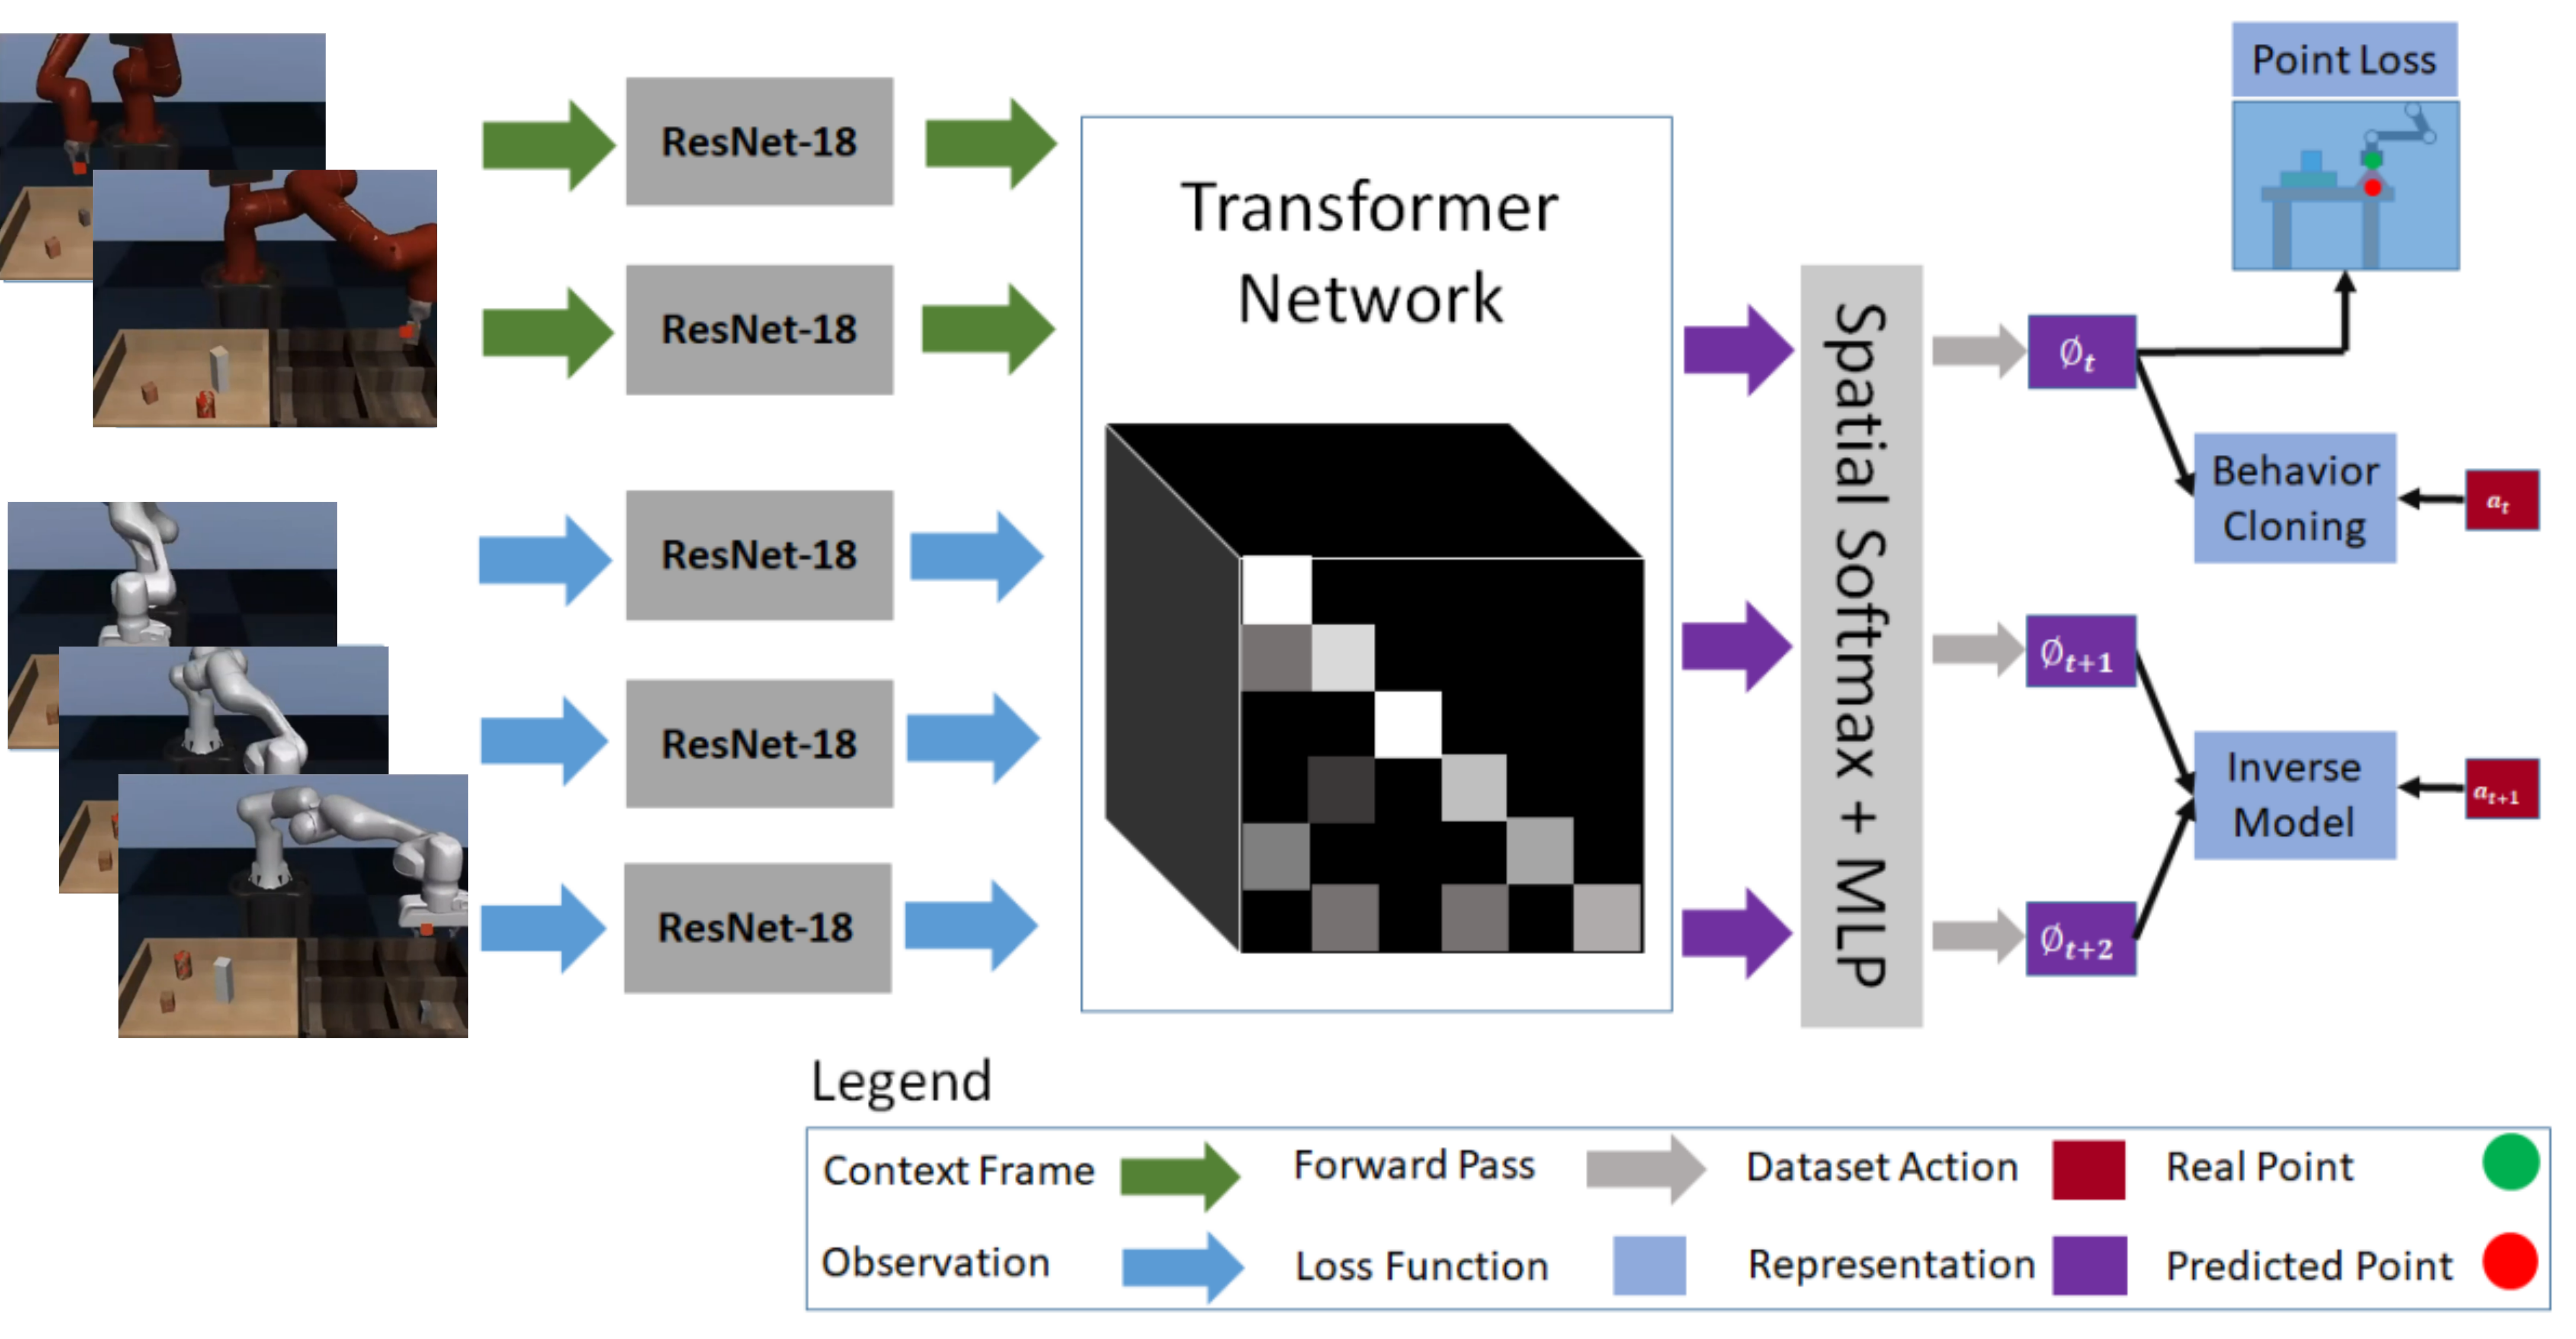
\includegraphics[width=0.7\textwidth]{figures/images/tosil/tosil_architecture.png}
    \caption{Transformer based architecture proposed in \cite{dasari2021transformers_one_shot}.  The Transformer network is used to create task-specific representation, given context and observation features computed with ResNet-18.}
    \label{fig:tosil_architecture}
\end{figure}

\begin{figure}[t]
    \centering
    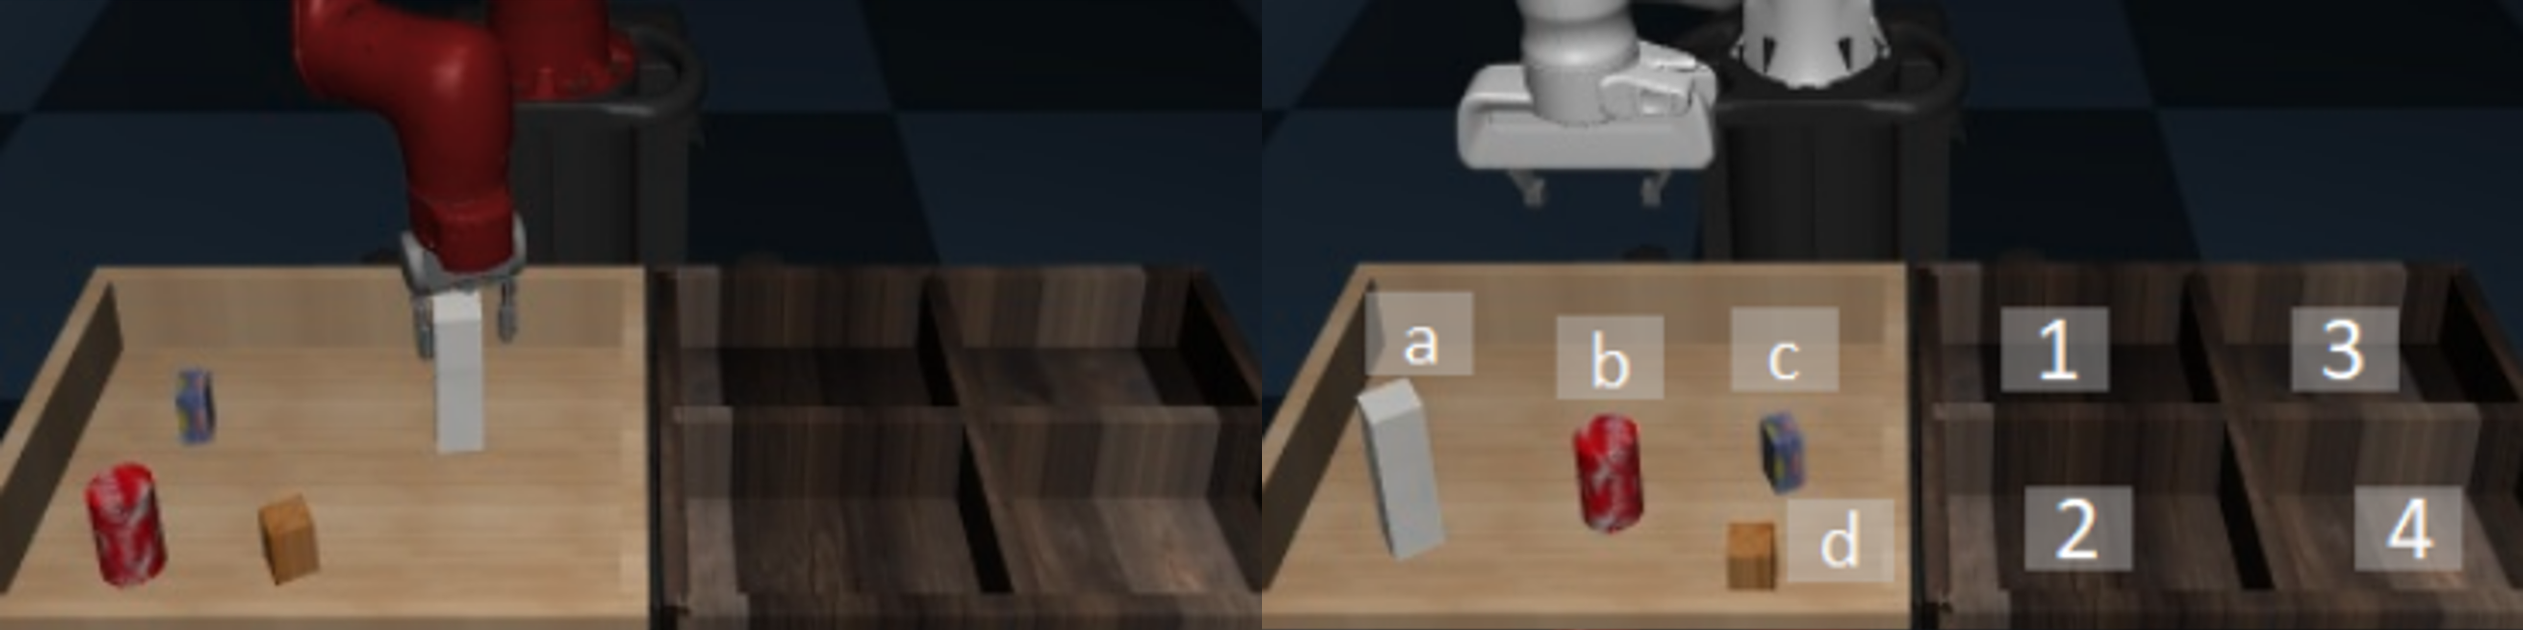
\includegraphics[width=0.7\textwidth]{figures/images/tosil/tosil_task.png}
    \caption{Validation setting proposed in \cite{dasari2021transformers_one_shot}. The
    16 tasks consist of taking an object (a-b) to a bin (1-4). On the left there is the demonstrator robot, while on the right there is the agent robot.}
    \label{fig:tosil_task}
\end{figure}

In \cite{mandi2022towards_more_generalizable_one_shot}, the authors presented MOSAIC (Multi-task One Shot imitation with self-AttentIon and Contrastive learning), which is an improvement of the work proposed in \cite{dasari2021transformers_one_shot} from both the architectural point-of-view and from the evaluation setting.
Indeed, from the architectural point of view, MOSAIC is designed to model a demonstration-conditioned policy, denoted as $\pi^{L}_{\theta}(a_{t}|s_{t},c)$, with $c$ representing the current task demonstration, such as a video depicting a robot performing the task. Specifically, the architecture is an optimization of TOSIL since, where the encoder-decoder Transformer architecture has been substituted with an encoder-only architecture leveraging the self-attention mechanism to correlate the embeddings coming from the current agent observation and the one coming from the demonstration frames (Figure \ref{fig:mosaic_architecture}). This adjustment allows to have a lower number of parameters and consequently improve the inference time. 
\begin{figure}[t]
    \centering
    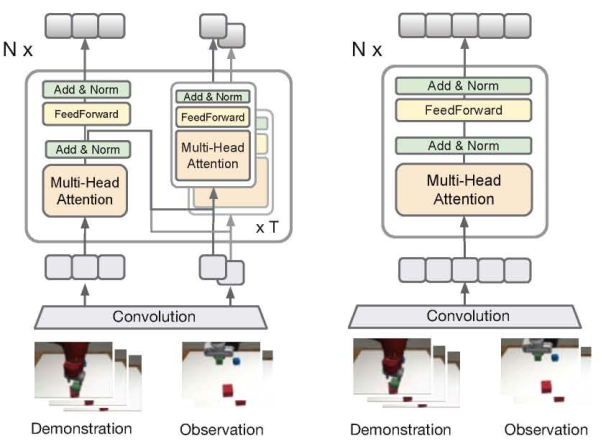
\includegraphics[width=0.7\textwidth]{figures/images/mosaic/architecture_comparison.png}
    \caption{(Left) The TOSIL architecture, as proposed in \cite{dasari2021transformers_one_shot}. (Right) The MOSAIC architecture, as introduced in \cite{mandi2022towards_more_generalizable_one_shot}. In the MOSAIC architecture, the original encoder-decoder Transformer architecture has been replaced with an encoder-only architecture featuring self-attention modules.}
    \label{fig:mosaic_architecture}
\end{figure}

\begin{figure}[t]
    \centering
    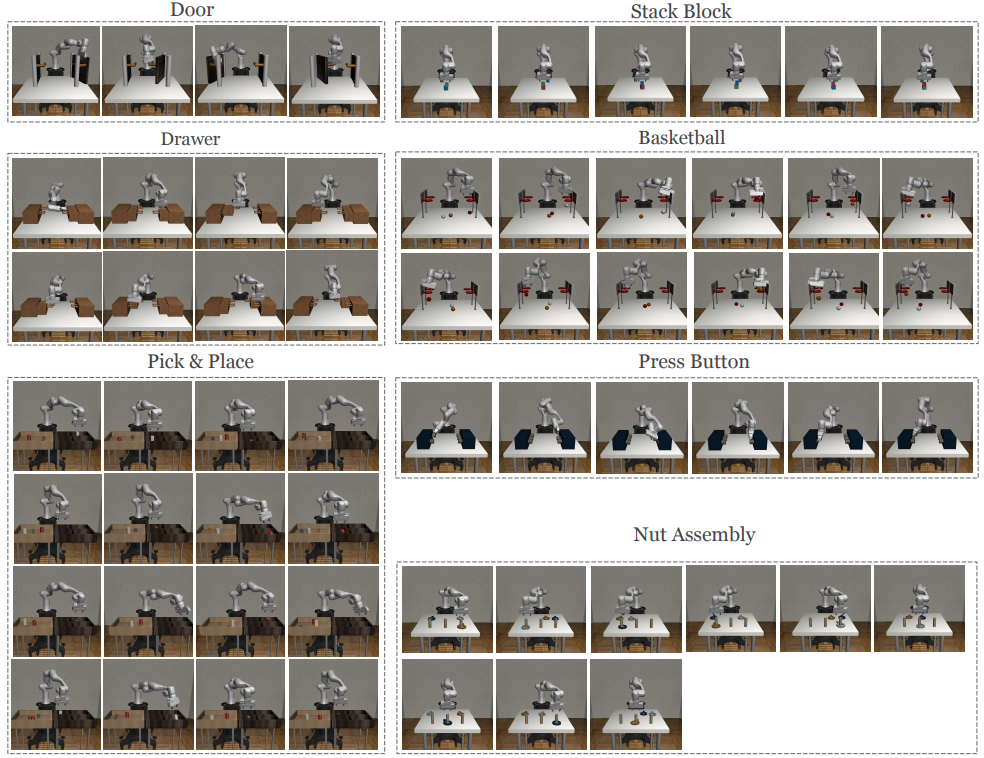
\includegraphics[width=0.7\textwidth]{figures/images/mosaic/mosaic_tasks.png}
    \caption{The evaluation tasks proposed in \cite{mandi2022towards_more_generalizable_one_shot} consist of a total of 7 tasks with 61 semantic variations.}
    \label{fig:mosaic_task}
\end{figure}

To handle this complex scenario involving both multiple variations and multiple tasks, the authors proposed training the system using a combination of loss functions. Specifically, in addition to the $\mathcal{L}_{BC}$ loss function defined in Formula \ref{eq:tosil_bc} and the $\mathcal{L}_{inv}$ loss function defined in Formula \ref{eq:tosil_inv}, the authors introduced a contrastive loss term implemented through the InfoNCE objective (Formula \ref{eq:mosaic_contrastive}). The goal of this loss is to enable the system to create similar representations for time-adjacent frames within a given task while maximizing the distance from representations corresponding to other tasks. In this context, $q$ is the anchor embedding obtained from a randomly sampled frame in a given batch $B$, $k_{+}$ is the positive example, which is a nearby frame from a different view of the batch (i.e., the original batch with a different data augmentation applied), and $k_{i}$ represents the negative samples, obtained from any other frame in the batch.

\begin{equation}
    \label{eq:mosaic_contrastive}
    \mathcal{L}_{Rep} = \log\left(\frac{\exp(q^TWk_{+})}{\exp(q^TWk_{+})+ \sum_{i=1}^{F-1}\exp(q^TWk_{i})}\right)
\end{equation}


To test the model, a dataset containing \textbf{seven distinct tasks} and \textbf{61 variations} (Figure \ref{fig:mosaic_task}) was generated by executing hand-written policies in a simulation environment. This dataset was employed to train and compare the proposed MOSAIC architecture against other one-shot (meta-)imitation learning methods, such as \cite{yu2018daml} and \cite{dasari2021transformers_one_shot}. The results, presented in Table \ref{table:mosaic}, demonstrate that MOSAIC surpasses previous methods in the Single-Task Zero-Shot Imitation Learning setting, particularly when addressing individual tasks with multiple variations and testing on previously unseen scenarios (i.e., novel object configurations).

Furthermore, when evaluated in a Multi-Task setting, where the system is trained on all tasks and subsequently tested on each task separately, MOSAIC exhibits the capability to partially replicate the demonstrated tasks. It is important to note that transitioning from a single-task to a multi-task context introduces inherent challenges. Despite being familiar with the tasks used during training, the success rate tends to decrease for almost all tasks. This phenomenon underscores the necessity for training procedures and architectures capable of generating embeddings that accurately represent both the task itself and its various sub-tasks. Such capacity is essential for reusing these embeddings when executing new instances or entirely novel tasks.

% \usepackage{graphicx}
% \usepackage{multirow}
% \usepackage{hhline}


\begin{table}[t]
    \scriptsize
    \selectfont
    \centering
    \caption{Results obtained in single-task and multi-task one-shot imitation learning \cite{mandi2022towards_more_generalizable_one_shot}.}
    \label{table:mosaic}
    \resizebox{\linewidth}{!}{%
    \begin{tabular}{|c|c|c|c|c|} 
    \hline
    Task & Setup & DAML \cite{yu2018daml} & TOSIL \cite{dasari2021transformers_one_shot} & MOSAIC \cite{mandi2022towards_more_generalizable_one_shot} \\ 
    \hhline{|=====|}
    \multirow{2}{*}{Open door} & single & 23.3~$\pm$ 5.2 & 57.9~$\pm$~7.1 & \textbf{67.1} $\pm$ \textbf{5.5} \\ 
    \cline{2-5}
     & multi & 10.8~$\pm$ 5.4 & 49.2~$\pm$ 6.0 & \textbf{68.3}~$\pm$~\textbf{6.3} \\ 
    \hhline{|=====|}
    \multirow{2}{*}{Open drawer} & single & 15.4~$\pm$ 5.5 & 57.5~$\pm$~3.9 & \textbf{65.4}~$\pm$~\textbf{3.4} \\ 
    \cline{2-5}
     & multi & 3.3~$\pm$~1.4 & 53.3~$\pm$~4.0 & \textbf{55.8}~$\pm$~\textbf{3.6} \\ 
    \hhline{|=====|}
    \multirow{2}{*}{Press button} & single & 62.8~$\pm$~3.9 & 56.4~$\pm$ 2.4 & \textbf{71.7}~$\pm$ \textbf{3.9} \\ 
    \cline{2-5}
     & multi & 1.7~$\pm$~0.7 & 63.3 $\pm$ 3.5 & \textbf{69.4}~$\pm$~\textbf{3.4} \\ 
    \hhline{|=====|}
    \multirow{2}{*}{Pick-and-Place} & single & 0.0~$\pm$~0.0 & 74.4~$\pm$~2.1 & \textbf{88.5}~$\pm$~\textbf{1.1} \\ 
    \cline{2-5}
     & multi & 0.0~$\pm$~0.0 & 19.5~$\pm$~0.4 & \textbf{42.1}~$\pm$ \textbf{2.3} \\ 
    \hhline{|=====|}
    \multirow{2}{*}{Stack block} & single & 10.0~$\pm$~1.8 & 13.3~$\pm$~2.6 & \textbf{79.3}~$\pm$~\textbf{1.8} \\ 
    \cline{2-5}
     & multi & 0.0~$\pm$~0.0 & 34.4~$\pm$~3.4 & \textbf{70.6}~$\pm$~\textbf{2.4} \\ 
    \hhline{|=====|}
    \multirow{2}{*}{Basketball} & single & 0.4~$\pm$~0.3 & 12.5~$\pm$~1.6 & \textbf{67.5}~$\pm$~\textbf{2.7} \\ 
    \cline{2-5}
     & multi & 0.0~$\pm$~0.0 & 6.9~$\pm$~1.3 & \textbf{49.7}~$\pm$~\textbf{2.2} \\ 
    \hhline{|=====|}
    \multirow{2}{*}{Nut assembly} & single & 2.2$\pm$~1.4 & 6.3 $\pm$~1.9 & \textbf{55.2}~$\pm$~\textbf{2.8} \\ 
    \cline{2-5}
     & multi & 0.0~$\pm$~0.0 & 6.3 $\pm$~1.3 & \textbf{30.7}~$\pm$~\textbf{2.5} \\
    \hline
    \end{tabular}
    }
    \end{table}

In this context, further improvements were introduced by the authors of \cite{chang2023one,cui2023from}. Specifically, the authors in \cite{chang2023one} analyze the shortcomings of existing methods like TOSIL and MOSAIC, which often struggle due to issues such as the DAgger problem (distribution shift from offline training), last-centimeter errors in fine motor control (e.g., collisions when the robot reaches the target object to pick), and misalignment with task contexts rather than the actual tasks (e.g., the system links the trajectories to the objects present in the scene rather than focusing on what is demonstrated by the expert).

To overcome these issues, the authors proposed a modular approach that separates task inference, i.e., understanding the intent of the demonstrations, from task execution, i.e., generating the actions to perform during the rollout. To achieve this, they introduced AWDA (Attributed Waypoints and Demonstration Augmentation), a modular framework for visual demonstration represented in Figure \ref{fig:awda_framework}. AWDA is based on two main concepts:

\begin{itemize}
    \item \textit{Attributed Waypoints}, designed to mitigate task execution errors, primarily those related to the distributional shift problem. These are classic waypoints (i.e., sequences of 6D poses of the end-effector) augmented with attributes, such as whether there is an object in the gripper. The robot moves between these generated waypoints using hand-defined motion primitives, which helps eliminate small errors during rollout execution that could otherwise cause the system to deviate from the correct trajectory.
    
    \item \textit{Demonstration Augmentation}, introduced to decouple tasks from task contexts. Specifically, two types of augmentation are introduced: \textbf{Asymmetric Demonstration Mixup}, which generates novel samples by mixing samples from two distinct trajectories according to Formula \ref{eq:awd_blanding}, where $v$ and $\tilde{v}$ are video demonstrations of two distinct tasks, and $o$ and $\tilde{o}$ are agent observations in two distinct contexts. \textbf{Additional Demonstrations via Trajectory Synthesis} involves generating free-space motions for the robot in various contexts by sampling a small number of points (1 to 3) uniformly at random within the agent's workspace and moving the end effector sequentially through these points using an inverse kinematics solver. Training samples are created by pairing each trajectory with itself, requiring the model to focus on the motion of the arm and ignore background elements to make correct predictions.
    
    \begin{equation}
        \label{eq:awd_blanding}
        v'_t = \alpha v_t + (1-\alpha) \tilde{v}_0 \quad o'_t = \alpha o_t + (1-\alpha) \tilde{o}_0
    \end{equation}
    
\end{itemize}
\begin{figure}[t]
    \centering
    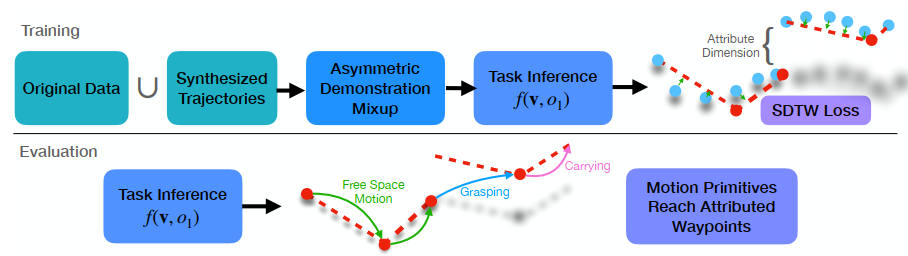
\includegraphics[width=0.9\textwidth]{figures/images/awda/awda_framework.png}
    \caption{AWDA framework proposed in \cite{chang2023one}. The task inference network $f(v,o)$ predicts a sequence of attributed waypoints (red dots) that are achieved by hand-defined motion primitives. The original data are augmented with free-space motion trajectories and asymmetric demonstration mixup in order to reduce the correlation between tasks and task content.}
    \label{fig:awda_framework}
\end{figure}


Using this framework, the authors trained the same Transformer-based architecture as in \cite{dasari2021transformers_one_shot}, achieving notable results. Specifically, on the pick-place task represented in Figure \ref{fig:tosil_task}, AWDA reached a success rate of \textbf{100}\% on two held-out variations, i.e., the system was trained on 14 variations and tested on the remaining 2. However, when tested on completely novel tasks, i.e., tasks never seen during training, the system struggled to succeed, as reported in Table \ref{table:awda_results}.
\begin{table}
    \centering
    \caption{Success rates achieved using the MOSAIC and AWDA methods. In this scenario, training is conducted on 5 out of the 6 tasks, with the remaining task reserved for testing.}
    \label{table:awda_results}
    \resizebox{\linewidth}{!}{%
    \begin{tabular}{|c|c|c|c|c|c|c|} 
    \hline
    Methods & Door & Drawer & Button & Blocks & Basketball & Nut Assembly \\ 
    \hhline{|=======|}
    MOSAIC & \textbf{0.05} & \textbf{0.15} & \textbf{0.05} & 0 & 0 & 0 \\ 
    \hline
    AWDA & \textbf{0.10} & \textbf{0.29} & 0.01 & 0 & 0 & \textbf{0.02} \\
    \hline
    \end{tabular}
    }
    \end{table}

In conclusion, significant research efforts have been dedicated to addressing the challenge of Visual Conditioned Multi-Task Imitation Learning (VC-MTIL). The aim is to develop systems capable of solving a given task in a zero-shot manner, starting from just a single video demonstration. Specifically, while these systems show promising results in solving new instances of seen tasks and unseen variations of known tasks, they struggle to handle a  multi-task multi-variation setting, exhibiting a consistent drop in performance. Additionally, they face difficulties in solving entirely new tasks.

Furthermore, the work discussed in this section predominantly involves experiments conducted in simulation environments, leaving unanswered whether these systems can be effectively applied in real-world settings, where demonstrations might also come in the form of human video demonstrations.

% \subsection{Object-Oriented Imitation Learning}
\label{sec:ooil}
All the methods discussed so far share a common characteristic: they are end-to-end systems that take high-level inputs, such as images, and directly generate the corresponding actions as output. While this approach can be sufficient in scenarios where the scene is simple, meaning there are no distracting objects, or if there are distracting objects, they can be easily identified by the system because they are consistently not involved in the manipulation, this end-to-end approach may struggle in more complex environments. Specifically, it can encounter difficulties when the robot workspace contains objects that are similar to each other, especially if these objects are involved in manipulation for some task variations.

Based on this consideration, this paragraph will describe methods that leverage \textbf{object priors}. Specifically, leveraging object priors means that the control policy is informed not only by the embedding of the agent scene, which is obtained from a deep architecture, but also by object-level information, such as the bounding boxes of objects in the scene, obtained from an object detector.

The concept of leveraging object priors has been explored in both earlier works \cite{devin2018deep,park2021object} and more recent approaches \cite{belkhale2023plato,zhu2023viola,zhu2023learning,jiang2023vima}.

One of the preliminary works on leveraging object priors was presented by the authors of \cite{devin2018deep}. This work primarily focuses on the challenge of generalization in Learning from Demonstration (LfD) systems that use an end-to-end approach. In such systems, a task-specific model is trained to predict actions based on raw visual observations. The authors found that while it is possible to achieve good \textit{instance-level generalization}, meaning the model can solve tasks with varying initial configurations using a limited number of samples, achieving \textit{category-level generalization} is more challenging. Category-level generalization refers to the model ability to solve tasks involving different objects. To achieve this, the dataset must include a large number of trajectories involving a wide variety of objects. For instance, if the task is to pour the contents of a bottle into a cup, the dataset should contain trajectories with different types of cups and bottles. However, constructing such a dataset is time-consuming and costly. Moreover, the potential of well-known large datasets in classical computer vision tasks, such as object detection, is not fully utilized.

To address this issue, the authors proposed a paradigm shift by introducing a robotic vision framework that operates on sets of objects rather than raw pixel data. This framework leverages prior datasets to learn a generic object concept model, thereby enhancing category-level generalization without requiring an extensive and diverse dataset. The framework is illustrated in Figure \ref{fig:object_prior_framework} and is composed of several stages:
\begin{itemize}
    \item \textbf{Meta-Attention}, which is basically a Region Proposal Network (RPN) \cite{fastrcnn}, trained on the well known MSCOCO \cite{lin2014microsoft} dataset. The RPN generates objects proposals, i.e., region of the image that possibly contain an object.
    \item \textbf{Task-Specific Attention}, which aims to learn what are the object of interest with respect to the task in hand. This module is parametreized as a vector $w$ such that the attention paid to $o^i$ is proportional to $e^{w^Tf(o^i)}$.
    \item \textbf{Soft Attention}, this module gives a probabilistic meaning to the atttention map obtained from the Task-Specific Attention. Specifically, a Boltzmann distribution is used to map the attention weights to a probability for each object proposal, i.e., $p\left(o^i \mid w_j\right)=\frac{e^{w_j^{\top} \frac{f\left(o^i\right)}{\left\|f\left(o^i\right)\right\|_2}}}{\sum_{i=0}^N e^{w_j^{\top} \frac{f\left(o^i\right)}{\left\|f\left(o^i\right)\right\|_2}}}$.
    \item \textbf{Movement Prediction Network}, this module predicts the next robot action, given the attended object information from the soft attention, and the robot state represented by the joint and end-effector state.
\end{itemize}
\begin{figure}[t]
    \centering
    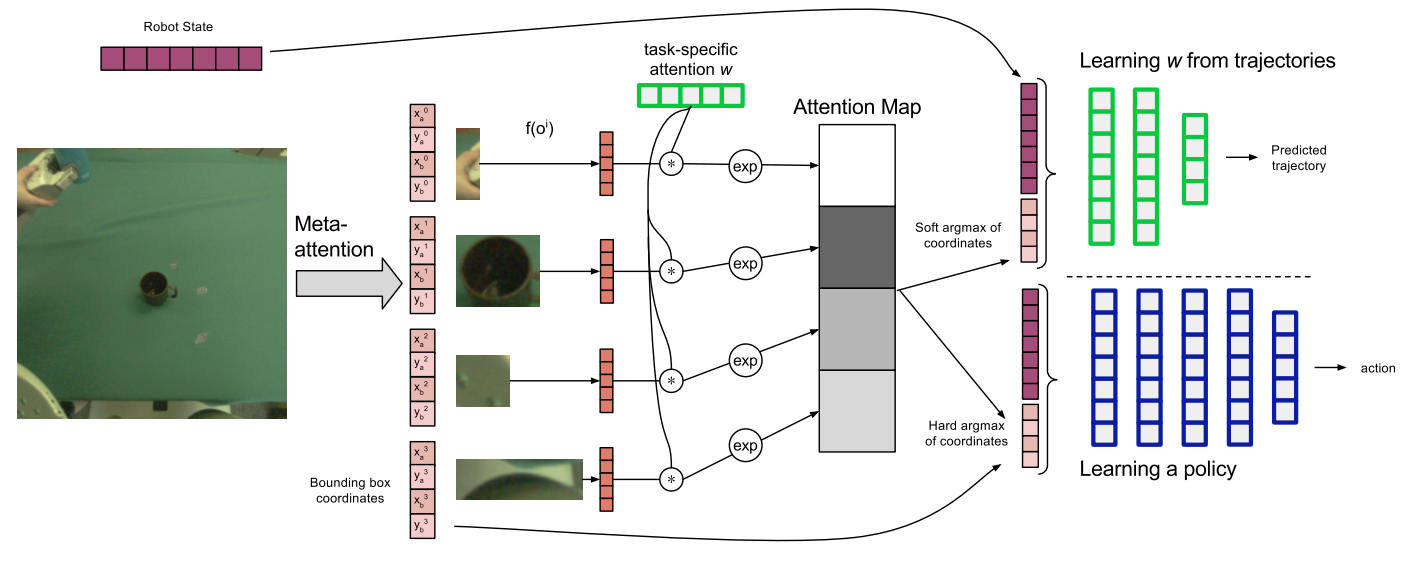
\includegraphics[width=0.8\textwidth]{figures/images/object_prior_framework.png}
    \caption{
            Robotic vision framework proposed in \cite{devin2018deep}. The framework is divided into different stages: \textbf{Meta-Attention}: Generates object proposals from an input image, trained on an object detection dataset, and shared across tasks; \textbf{Task-Specific Attention}: Focuses on relevant objects for a task using the meta-attention's semantic features; \textbf{Soft Attention}: Distributes attention as probabilities over object proposals using a Boltzmann distribution; \textbf{Movement Prediction Network}: Combines attended object information with the robot's state to predict the next action.
        }
    \label{fig:object_prior_framework}
\end{figure}
This preliminary work focused mainly on two tasks:
\begin{itemize*}
    \item  \textit{Pouring Task}: The robot is required to pour contents from a bottle into a mug. The challenge is to locate the mug from an image without being explicitly provided its location, especially when different mugs are used during training and testing.
    \item \textit{Sweeping Task}: The robot must sweep an object (e.g., a plastic orange) into a dustpan, with both objects starting in different positions. This task requires the robot to adapt its approach based on the relative positions of the objects.
\end{itemize*}
During testing, the authors focused on \textit{Category Generalization} and the ability to \textit{Ignore Distractor Objects}. For the former, the system was trained with only one type of mug and evaluated with other mugs (Figure \ref{fig:pouring_task_setting}). The results showed that the system successfully poured the contents into the correct mug, thanks to the learned task-specific attention weight that highlighted the mug features. For the latter, the authors designed a test where two mugs were present in the scene (Figure \ref{fig:task_specific_attention}). Since the model did not receive any conditioning signal indicating which mug to use, the authors fine-tuned the attention weight on trajectories where only the brown mug was used, demonstrating that this mechanism could focus on more specific features, such as the mug color.
\begin{figure}[t]
    \centering
    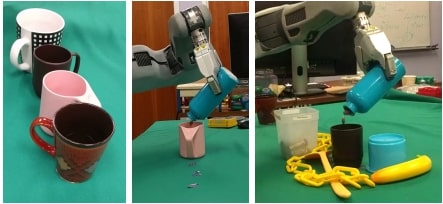
\includegraphics[width=0.6\textwidth]{figures/images/deep_object_centric_representation/pouring_task.jpg}
    \caption{Pouring task setting proposed in \cite{devin2018deep}. (Left) Mugs used for evaluation. Note that only the brown mug was seen during training. Center: Successful pouring into the pink mug. (Right) Pouring into the brown mug in a cluttered environment that was not seen during training.}
    \label{fig:pouring_task_setting}
\end{figure}

\begin{figure}[t]
    \centering
    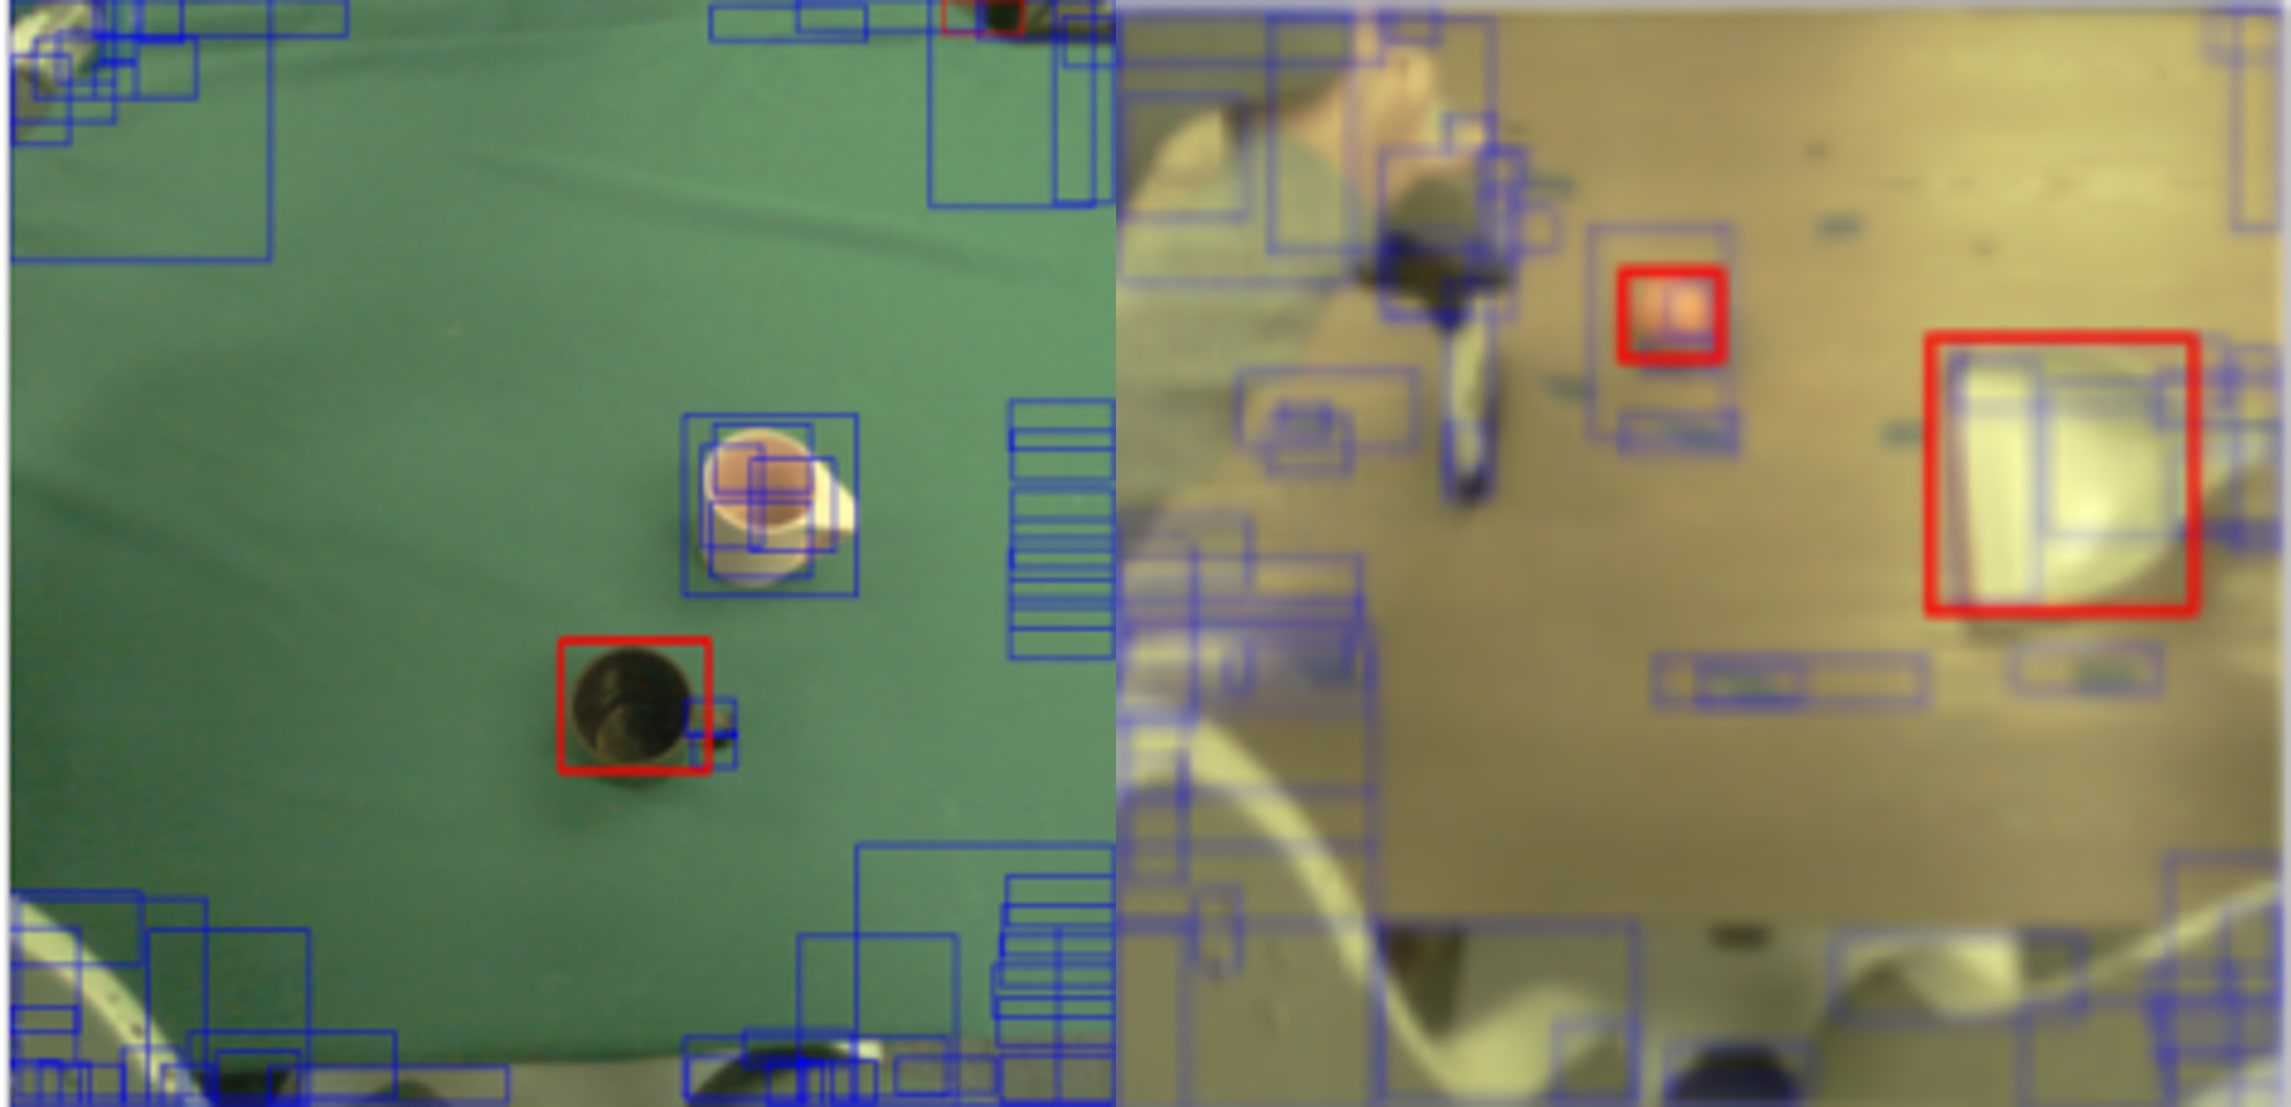
\includegraphics[width=0.6\textwidth]{figures/images/deep_object_centric_representation/mugs_distractors.jpg}
        \caption{The region proposals (meta-attention) are drawn in blue and the task-specific attended regions are drawn in red. For the Pouring task with distractor mug (pink) and target mug (brown), the attention locks on to the brown mug as its position defines the trajectory. For the sweeping task, two attention vectors are used, one attends to the orange and one attends to the dustpan.}
    \label{fig:task_specific_attention}
\end{figure}

In summary, this preliminary work demonstrated that leveraging object priors can facilitate category-level generalization by utilizing large, well-known datasets for the object-detection problem. However, the experimental setup was relatively simple, even in scenarios with distractor objects. The proposed system could handle distractor objects only after specific fine-tuning and was not able to dynamically discriminate between objects of interest and distractors based on task variations.

A recent work that follows a similar approach is proposed in \cite{zhu2023viola}. In this work, the authors introduced VIOLA (Visuomotor Imitation via Object-centric Learning) (Figure \ref{fig:viola_architecture}), an architecture inspired by the ideas presented in \cite{devin2018deep}. VIOLA uses an RPN and a ResNet18 \cite{resnet} to generate object proposals and produce a spatial feature map, respectively. It then constructs a \textit{per-step feature} vector, composed of three key elements: a \textbf{global context feature} that encodes the current task stage, an \textbf{eye-in-hand visual feature} to mitigate occlusion, and a \textbf{proprioceptive feature} that captures the robot state. These per-step features are concatenated to form a \textbf{history of observations}, which is designed to capture temporal dependencies and dynamic changes in object states. This tensor is then fed into a Transformer \cite{vaswani2017attention}, which leverages its intrinsic attention mechanism to automatically focus on the object of interest.
\begin{figure}[t]
    \centering
    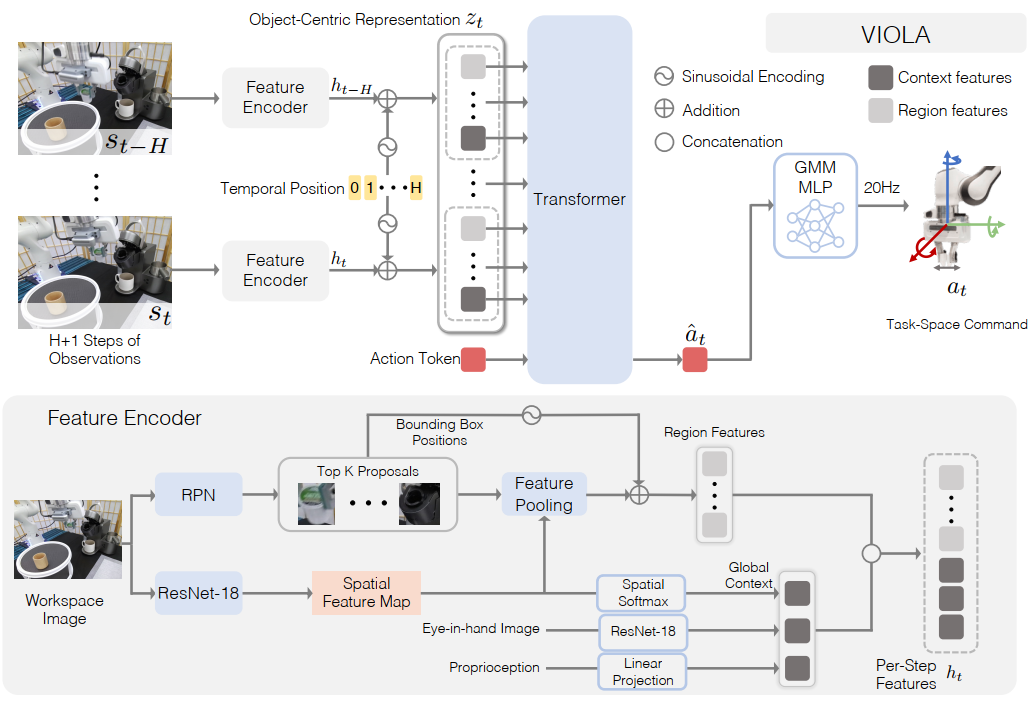
\includegraphics[width=0.7\textwidth]{figures/images/viola/viola_architecture.png}
        \caption{The VIOLA architecture proposed in \cite{zhu2023viola}. (Top) The overall control architecture is based on a Transformer module that processes a stack of \textit{per-step features} $h_{t}$, obtained from the Feature Encoder, to generate a final action embedding, which is then input into a GMM policy. (Bottom) The Feature Encoder builds both local and global features. Local features correspond to regions of interest extracted by the RPN. Global features are obtained by processing the workspace image, the image from the camera on the gripper, and proprioceptive information.
        }
    \label{fig:viola_architecture}
    
\end{figure}

\begin{figure}[t]
    \centering
    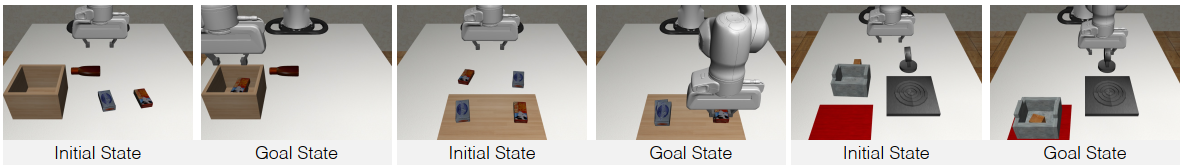
\includegraphics[width=0.9\textwidth]{figures/images/viola/viola_task.png}
    \caption{Simulation tasks on which the VIOLA \cite{zhu2023viola} method was tested. (Left) Sorting task. (Center) Stacking task. (Right) BUDS-Kitchen task}
    \label{fig:viola_task}
    
\end{figure}

This method was first evaluated in a simulation environment across three tasks, as depicted in Figure \ref{fig:viola_task}. Various testing scenarios were considered, including different object placements, the introduction of distractor objects, and changes in camera position. Generally speaking, VIOLA outperformed all baselines across these testing conditions, further demonstrating the utility of object priors in enhancing the robustness of such methods. However, similar to \cite{devin2018deep}, the testing scenarios were relatively simple, with clear distinctions between distractors and objects of interest. The distractors were objects never seen during the demonstration and were not involved in manipulation, making them relatively easy for the model to discriminate.

In the works discussed so far, the approach has primarily focused on leveraging object priors to directly predict the actions that the robot must perform. However, a different approach was proposed in \cite{belkhale2023plato}, where the authors introduced an alternative interpretation of object-centric concept. Instead of focusing on the robot perspective, they shifted the emphasis to the object perspective, proposing PLATO (Predicting Latent Affordances Through Object-Centric Play). PLATO is a learning framework that learns a \textbf{latent affordance space}, which describes how an object can be used (e.g., a block being grasped, a door knob being turned, or a drawer being opened).

The authors argue that learning these affordances (i.e., what happens to the object) rather than plans (i.e., what happens to the robot) from play leads to a simpler and more robust task representation that can operate over varying time horizons. This, in turn, results in more effective policies at test time. This paradigm shift allows the policy to reason about the environment more effectively: given access to an affordance (e.g., the door knob being turned) and a goal (e.g., an opened door), the policy can work backwards to infer the behavior needed to exploit that affordance (e.g., reaching the knob and rotating the gripper to turn it).

To reach this objective authors started from the observation that a single-object manipulation is composed of the following three phases:
\begin{enumerate}
    \item \textbf{Pre-interaction}, when the robot prepares to interact with an object (e.g., reaching for a block).
    \item \textbf{Interaction}, when the robot and the object engage in joint actions (e.g., pushing or pulling the block).
    \item \textbf{Post-interaction}, when the robot separates from the object, and the object may come to rest (e.g., the block stops moving).
\end{enumerate}
Given these three phases, the algorithm learns a \textbf{latent affordance distribution}. Specifically, the architecture comprises three learnable modules: \( E \), \( E' \), and \( \pi \). \( E \) models the posterior distribution, mapping the full interaction trajectory \( \tau^{i} \) to the corresponding latent affordance distribution, from which the affordance embedding \( z \) is sampled. \( E' \) is the prior module used during rollout. It takes the current state and the goal state as input and generates the affordance embedding \( z' \). This module is trained to match the posterior distribution modeled by \( E \). \( \pi \) represents the current policy, which generates the action \( a^{i} \) given the current state \( s^{i} \), the desired goal \( o_g \), and the latent embedding \( z \).

These three modules are trained end-to-end by minimizing the loss function in Formula \ref{eq:plato_equation}, which includes three terms. The first two terms correspond to the policy \( \pi \), ensuring it matches the ground-truth trajectories in the interaction and pre-interaction phases. The last term is the KL-divergence, used to train the posterior and prior modules \( E \) and \( E' \).

\begin{equation}
    \label{eq:plato_equation}
    \begin{aligned}
        \mathcal{L}_{PLATO} = -\log \left(\pi\left(a_{1: H}^{(i)} \mid s_{1: H}^{(i)}, o_g, z\right)\right)- \\ 
        \alpha \log \left(\pi\left(a_{1: H}^{(-)} \mid s_{1: H}^{(-)}, o_g, z\right)\right)+ \\ 
        \beta \operatorname{KL}\left(p(z) \| p\left(z^{\prime}\right)\right)
    \end{aligned}
\end{equation}
\begin{figure}[t]
    \centering
    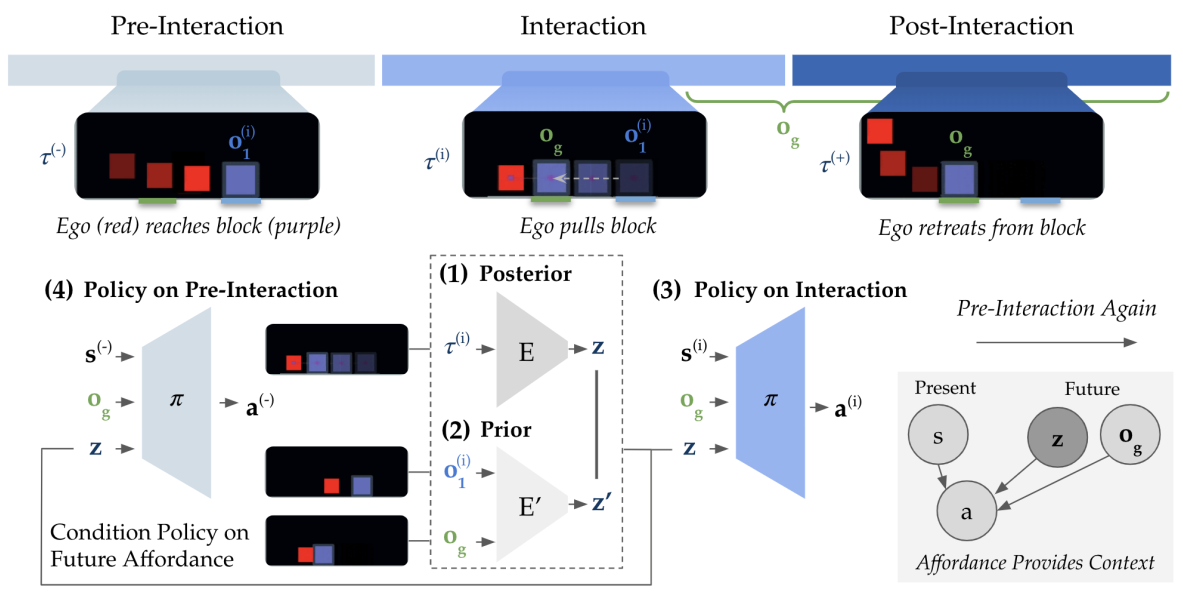
\includegraphics[width=0.7\textwidth]{figures/images/plato/plato.png}
    \caption{PLATO architecture proposed in \cite{belkhale2023plato}. The architecture is composed of different stages. (1) The posterior encoder \( E \) encodes the interaction sequence \( \tau^{(i)} \) into the affordance \( z \). (2) The prior encoder \( E' \) encodes the object initial state \( o^{(i)}_1 \) and goal state \( o_g \) to predict \( z \), with \( o_g \) sampled after the interaction. (3) The policy is trained to output actions during the interaction period conditioned on the affordance. Simultaneously, (4) it is trained to output actions during the pre-interaction period conditioned on the ``future" affordance.
    }
    \label{fig:plato}
    
\end{figure}

\begin{figure}[t]
    \centering
    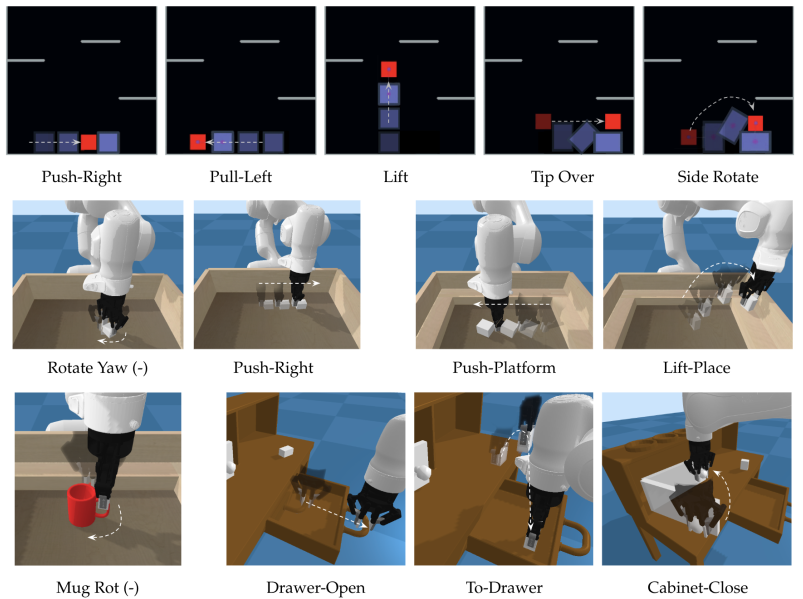
\includegraphics[width=0.7\textwidth]{figures/images/plato/tasks.png}
    \caption{ Testing scenarios and primitives proposed in \cite{belkhale2023plato}. (Top) \textbf{Block2D} Environment primitive examples. (Center) \textbf{Block3D} and \textbf{Block3DPlatform} primitive examples. (Bottom) The left image shows an example primitive in \textbf{Mug3D-Platforms}. The right three images show sample tasks from \textbf{Playroom3D}.}
    \label{fig:plato_task}
    
\end{figure}

Finally, this method was tested in a variety of scenarios, including both single-object and multiple-object manipulation with different manipulation primitives (Figure \ref{fig:plato_task}). However, in the multi-object scenarios, the system was only tested on single-object manipulation primitives.

This work is particularly noteworthy as it demonstrates that a policy can be learned by solving an inverse problem, starting from object affordances and deriving the corresponding robot trajectories. It also shows that the policy can be conditioned based on the desired goal state. However, certain aspects were not addressed in this work, such as the potential presence of distractor objects and tasks requiring the manipulation of multiple objects. Additionally, the affordances were learned in the object space (i.e., with known object poses) rather than in the high-level image space.

The works discussed in this paragraph highlight the significant research efforts aimed at modeling the manipulation problem from an object-centric perspective. These efforts either focus on the affordances of the object (i.e., the possible movements the object allows) or introduce object priors defined by regions of interest that may contain the object to be manipulated, with results demonstrated in both simulated and real-world environments. However, the methods presented so far primarily address single-task scenarios, where distractor objects can be easily identified as they remain constant across demonstrations. In contrast, this thesis proposes a solution for a more challenging scenario in which the robot operates in a multi-variation environment. This environment includes multiple similar objects, which may serve as either targets or distractors depending on the specific task variation.

\section{Problem formulation}
\label{sec:ocpl_problem}
As described in Section \ref{sec:occp_related_works}, this thesis primarily addresses the problem of Visual-Conditioned Multi-Task Imitation Learning. The goal is to train a single conditioned control function, $\pi_{\theta}(a_{t}| o^{a}_{t}, c_m)$, that can guide a robotic agent in solving both variations of a given task and entirely different tasks. Where, the input consists of a command $c_m$, represented as a video demonstration of the requested task, along with the current observation of the agent $o^{a}_{t}$.

The approach proposed in this thesis is based on the observation that solving this problem involves two key tasks:
\begin{itemize}
    \item \textit{Command analysis}: This task involves solving a cognitive problem, where the system must interpret the high-level task command, understand the task intent, identify the relevant objects, and recognize the required actions.
    \item \textit{Action generation}: This task involves solving a control problem, where the system must correlate the information from the command analysis with the agent environmental state to generate a valid action that moves the robot toward completing the requested task.
\end{itemize}

As demonstrated in the comprehensive review of related works (Section \ref{sec:occp_related_works}), the Visual-Conditioned MTIL problem is typically addressed using end-to-end architectures, which are trained with an action-centric behavioral cloning loss. While these systems are often able to control the robot and produce \textbf{reasonable trajectories} to complete tasks like pick-and-place, they may manipulate the wrong object, indicating a limitation in the cognitive ability to correctly identify the relevant object.


In this thesis, a modular approach is adopted. Specifically, Figure \ref{fig:end_to_end_vs_modular} illustrates the differences between a general end-to-end architecture and the proposed modular architecture. In the end-to-end architecture, the \textit{Backbone Module}, which can be any deep learning architecture used in state-of-the-art methods, takes both the agent observation $o^{a}_t$ and the command $c_{m_i}$ as input. It generates an embedding $z_t$ that must encapsulate all the necessary information for the \textit{Control Module} to produce a valid action. This includes details derived from both the command, such as the position of the object of interest, the task being solved, its variations, as well as the state of the agent itself.

In contrast, the modular approach utilizes two backbone modules. The first, the \textit{Command Analysis Backbone}, explicitly solves the cognitive task, producing task-relevant information ($z^{task}_t$) such as the position of the object of interest. The second, the \textit{Control Backbone Module}, generates a control embedding ($z^{control}_t$), which directly encodes information relevant to the action to be performed. In this modular approach, the \textit{Control Module} takes both the task-relevant information ($z^{task}_t$) and the control embedding ($z^{control}_t$) as inputs.

\begin{figure}[t]
    \centering
    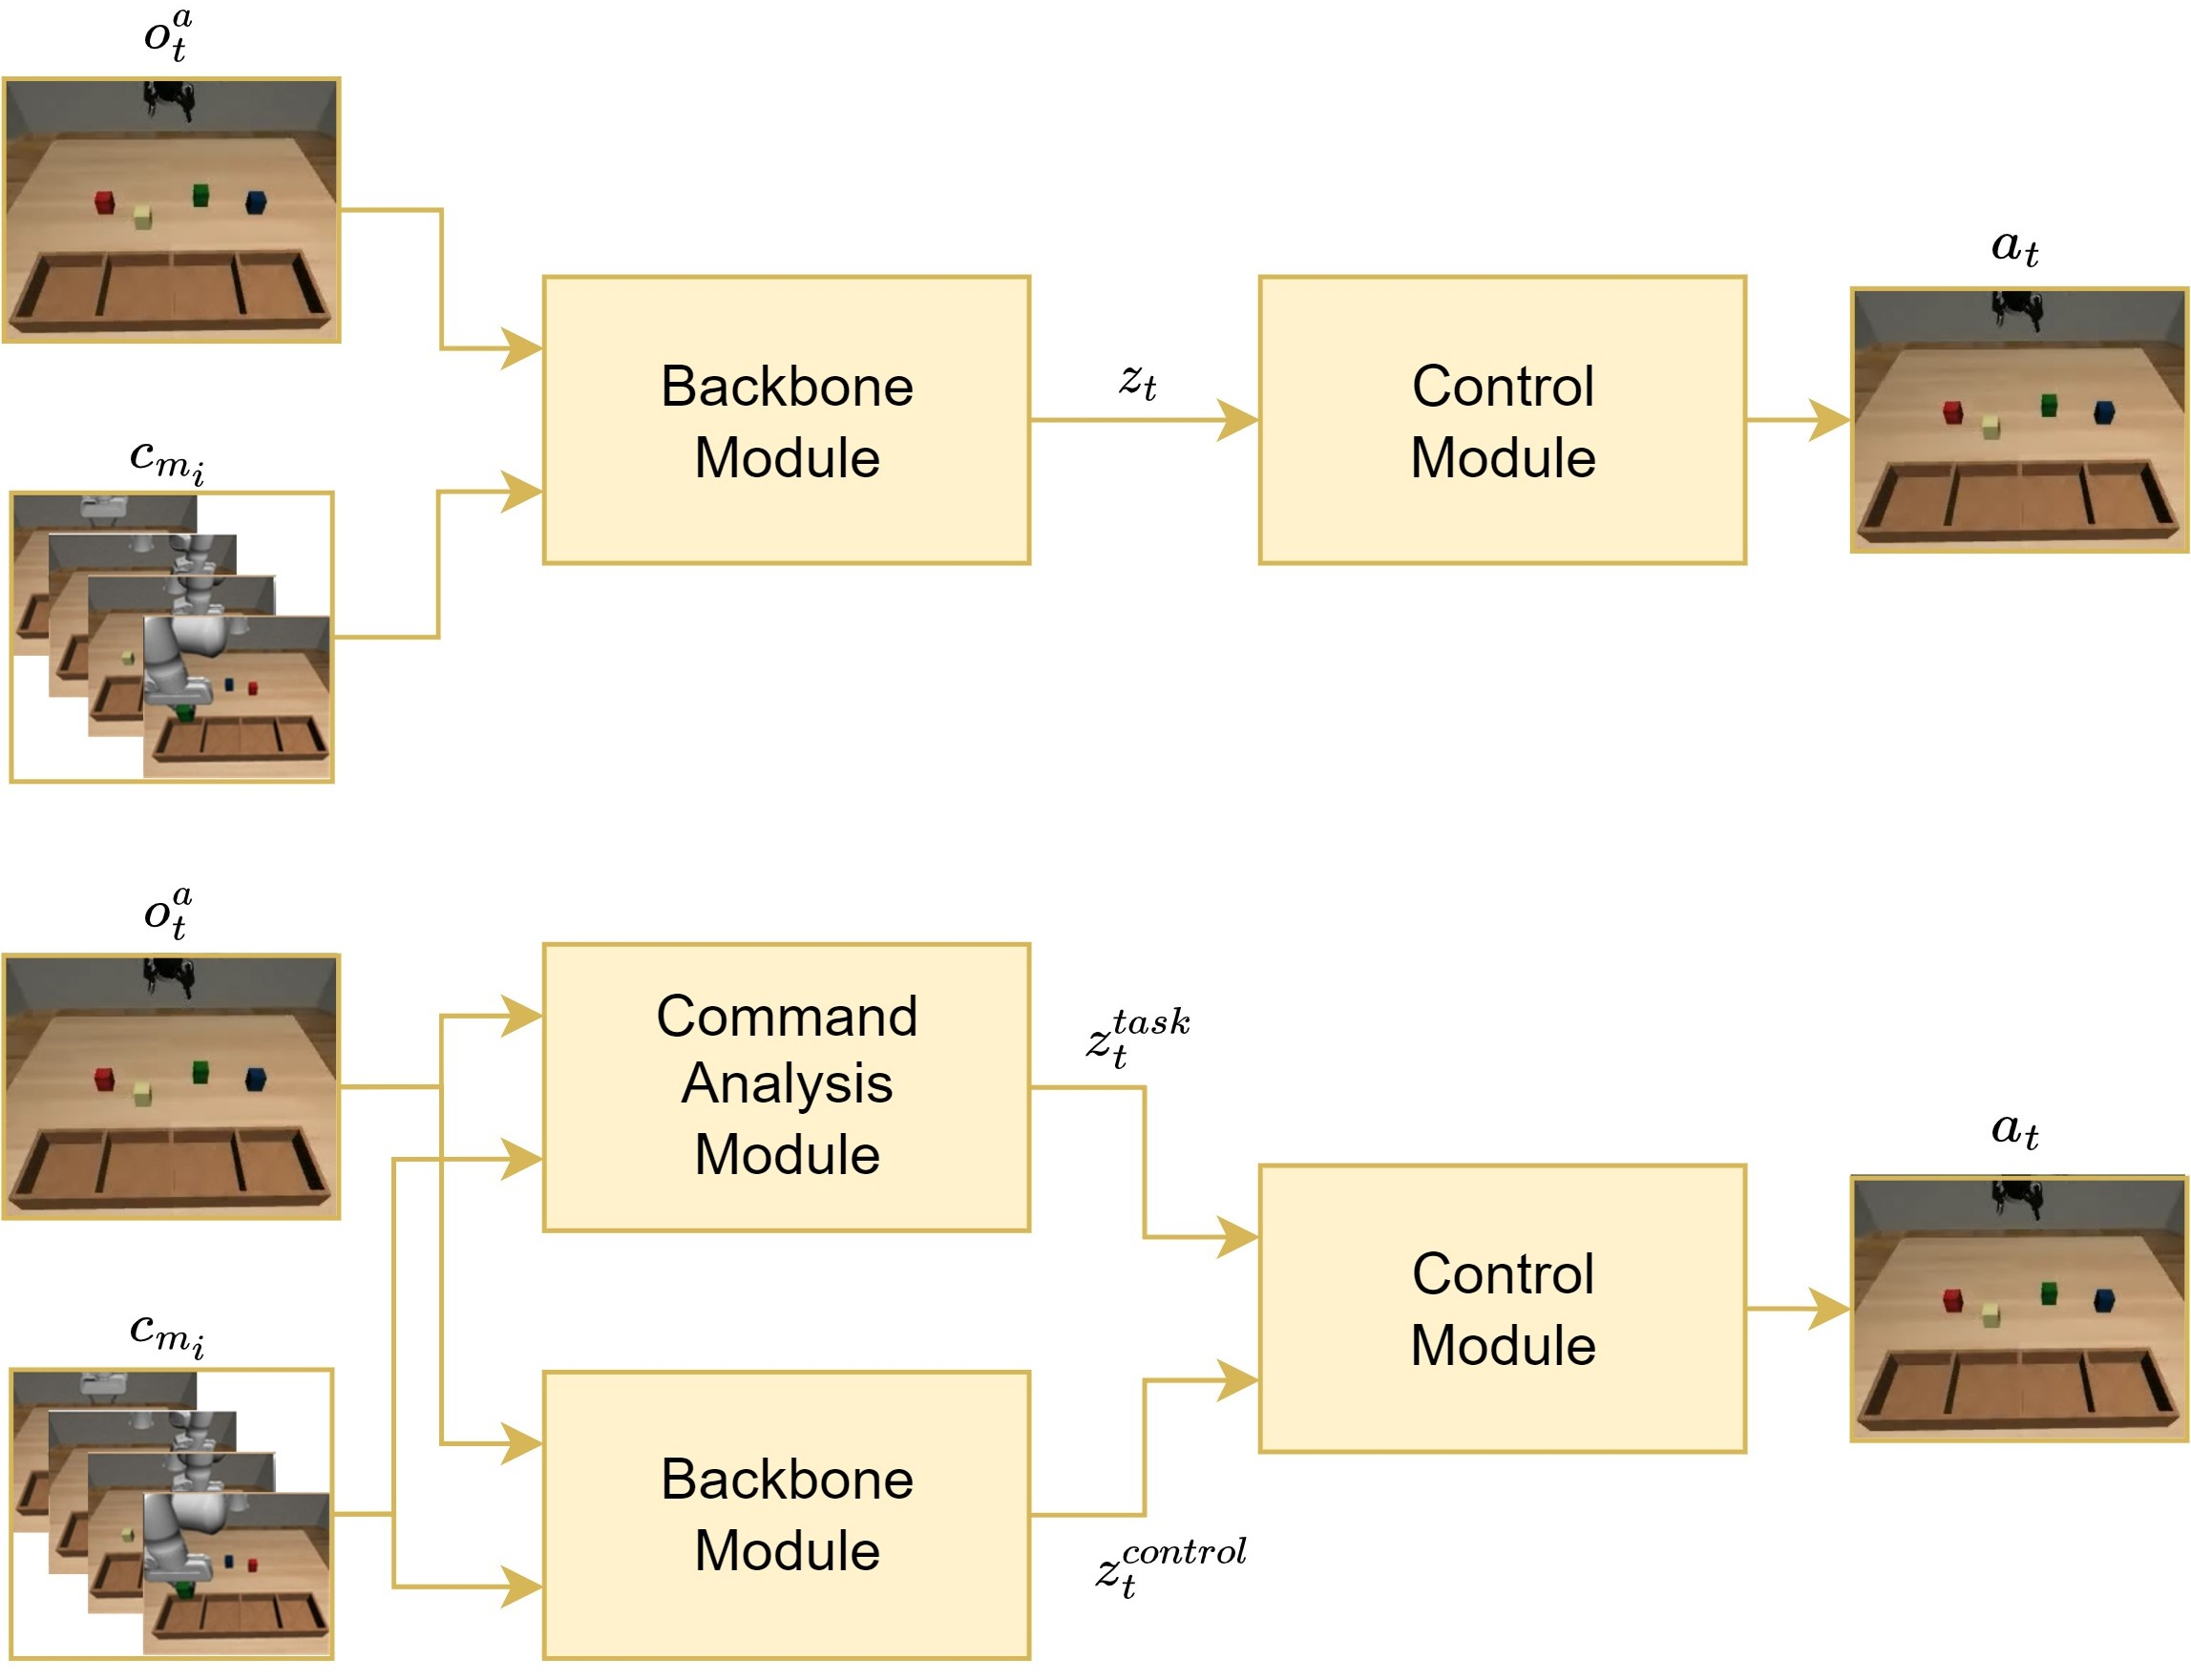
\includegraphics[width=0.7\textwidth]{figures/images/ch3/end_to_end_vs_modular.jpg}
    \caption{(Upper) General end-to-end architecture, where the \textit{Backbone Module} takes as input both the agent observation and the command. It generates an embedding $z_{t}$ that must contain information related to both the command and the control. (Bottom) In the modular architecture, there are two backbone modules: the \textit{Command Analysis Module}, which generates the task-embedding $z^{task}_t$, and the \textit{Backbone Module}, which is trained to generate only the control-embedding $z^{control}_{t}$.}
    \label{fig:end_to_end_vs_modular}
\end{figure}


The underlying assumption of this approach is that by separating the problem into two components, cognitive and control, and designing task-specific modules trained independently of each other, the system becomes more robust. For example, the Command Analysis Module is trained specifically for the cognitive task (e.g., the Conditioned Object Detection task described in Chapter \ref{ch:cod}), while the Control Backbone is trained for the control task. This separation allows the final Control Module to be informed by optimal embeddings generated by modules trained on task-specific problems.

Section \ref{sec:} provides an example of a cognitive problem that can be addressed by the Command Analysis Backbone. Here, the focus is on describing the problem solved in order to learn the final control policy $\pi_{\theta}$. Specifically, the goal is to learn the parameters of the policy $\pi_{\theta}$ using a supervised-learning approach.

The first step is defining the dataset. As explained in Section \ref{sec:bc}, in multi-task, multi-variation scenario, there are $n$ distinct tasks, denoted by $\mathcal{T} = \left\{T_{1}, T_{2}, \dots, T_{n}\right\}$, where each task $T_{i}$ is associated with a set of variations $\mathcal{M}_{i}$. For each task, a specific dataset $\mathcal{D}_{i} = ((c_{m}, \tau_{m}), m \in \mathcal{M}_{i})$ is constructed, containing pairs of demonstrator videos $c_{m}$ and corresponding target trajectories $\tau_{m}$ for each variation. The demonstrator video consists solely of visual observations, represented as $c_{m} = \left\{o^{d}_{1}, o^{d}_{2}, \dots, o^{d}_{T'}\right\}$, while the target trajectory includes both observations and associated actions: $\tau_{m} = \left\{(o^{a}_{1},a_{1}), \dots, (o^{a}_{T}, a_{T})\right\}$.

Building upon the complete dataset $\mathcal{D} = \left\{\mathcal{D}_{1}, \dots, \mathcal{D}_{n}\right\}$, the optimal parameters $\theta^{*}$ are obtained by solving the minimization problem described in Formula \ref{eq:minimization_prob}, where the loss function $\mathcal{L}$ is minimized.
\begin{equation}
    \label{eq:minimization_prob}
    \theta^{*} = \underset{\theta}{\text{arg} \ \min} \ \mathcal{L}(\pi_{\theta}, \mathcal{D})
\end{equation}

Section \ref{sec:ocpl_architecture} will present the specific instance of the proposed architecture, along with the loss function and modules used. The results of the experiments will be discussed in Section \ref{sec:ocpl_experimental}.

\section{Proposed Architecture}
\label{sec:ocpl_architecture}
This section provides the effective implementation of the general modular architecture described in Section \ref{sec:cod_problem}. Since the Command Analysis task being solved is Conditioned-Object Detection (Chapter \ref{ch:cod}), the focus here is on how the COD module is effectively integrated into the control framework.

The COD module is integrated into two different architectures, which vary in the number of control modules they use. Section~\ref{sec:ocpl_architecture_scm} outlines an architecture that employs a single control module to predict actions for the entire trajectory. In contrast, Section~\ref{sec:ocpl_architecture_dcm} describes an architecture that splits the control module into two distinct parts: one for computing actions during the reaching phase, and another for the final phase, where the specific primitive depends on the task.

\subsection{Single control module}
\label{sec:ocpl_architecture_scm}
The architecture (Figure \ref{fig:single_control_module}) composed of a single control module is essentially an instance of the general modular architecture depicted in Figure \ref{fig:end_to_end_vs_modular}. Specifically, the Command Analysis Module is replaced by the CTOD module (Section \ref{sec:cod_tod}), which takes as input the current agent observation $o^a_t$ and the command $c_m$, producing a task embedding represented by the \textit{target-object bounding box}, i.e., $z^{task}_t = bb^{target}_t$.

The Backbone Module, responsible for generating the control embedding $z^{control}_{t}$, is replaced by the same backbone used in MOSAIC. This backbone is a combination of a Convolutional Network, which encodes the agent observation $o^a_t$ and the demonstration frames $c_m$, and a Self-Attention mechanism to create correlated agent and command embeddings (Section \ref{sec:bc}). 

Finally, the Control Module follows the same implementation as in MOSAIC \cite{mandi2022towards_more_generalizable_one_shot}. In this case, the actions generated by the control module are sampled from a multivariate logistic distribution (Equation \ref{equation:logistic_distribution}), where the distribution parameters $\mu_{i}$ and $\sigma_{i}$ are estimated by MLPs implementing the Control Module.

\begin{equation}
    \label{equation:logistic_distribution}
    a_{t} \sim \sum_{i=1}^{m} \alpha(z_t) \, logistic(\mu_{i}(z_t), \sigma_{i}(z_t))
\end{equation}

Here, the embedding $z_t$ is a concatenation of $z^{control}_{t}$, generated by the MOSAIC Backbone, and $bb^{target}_t$, produced by the CTOD Module.

\begin{figure}[t]
    \centering
    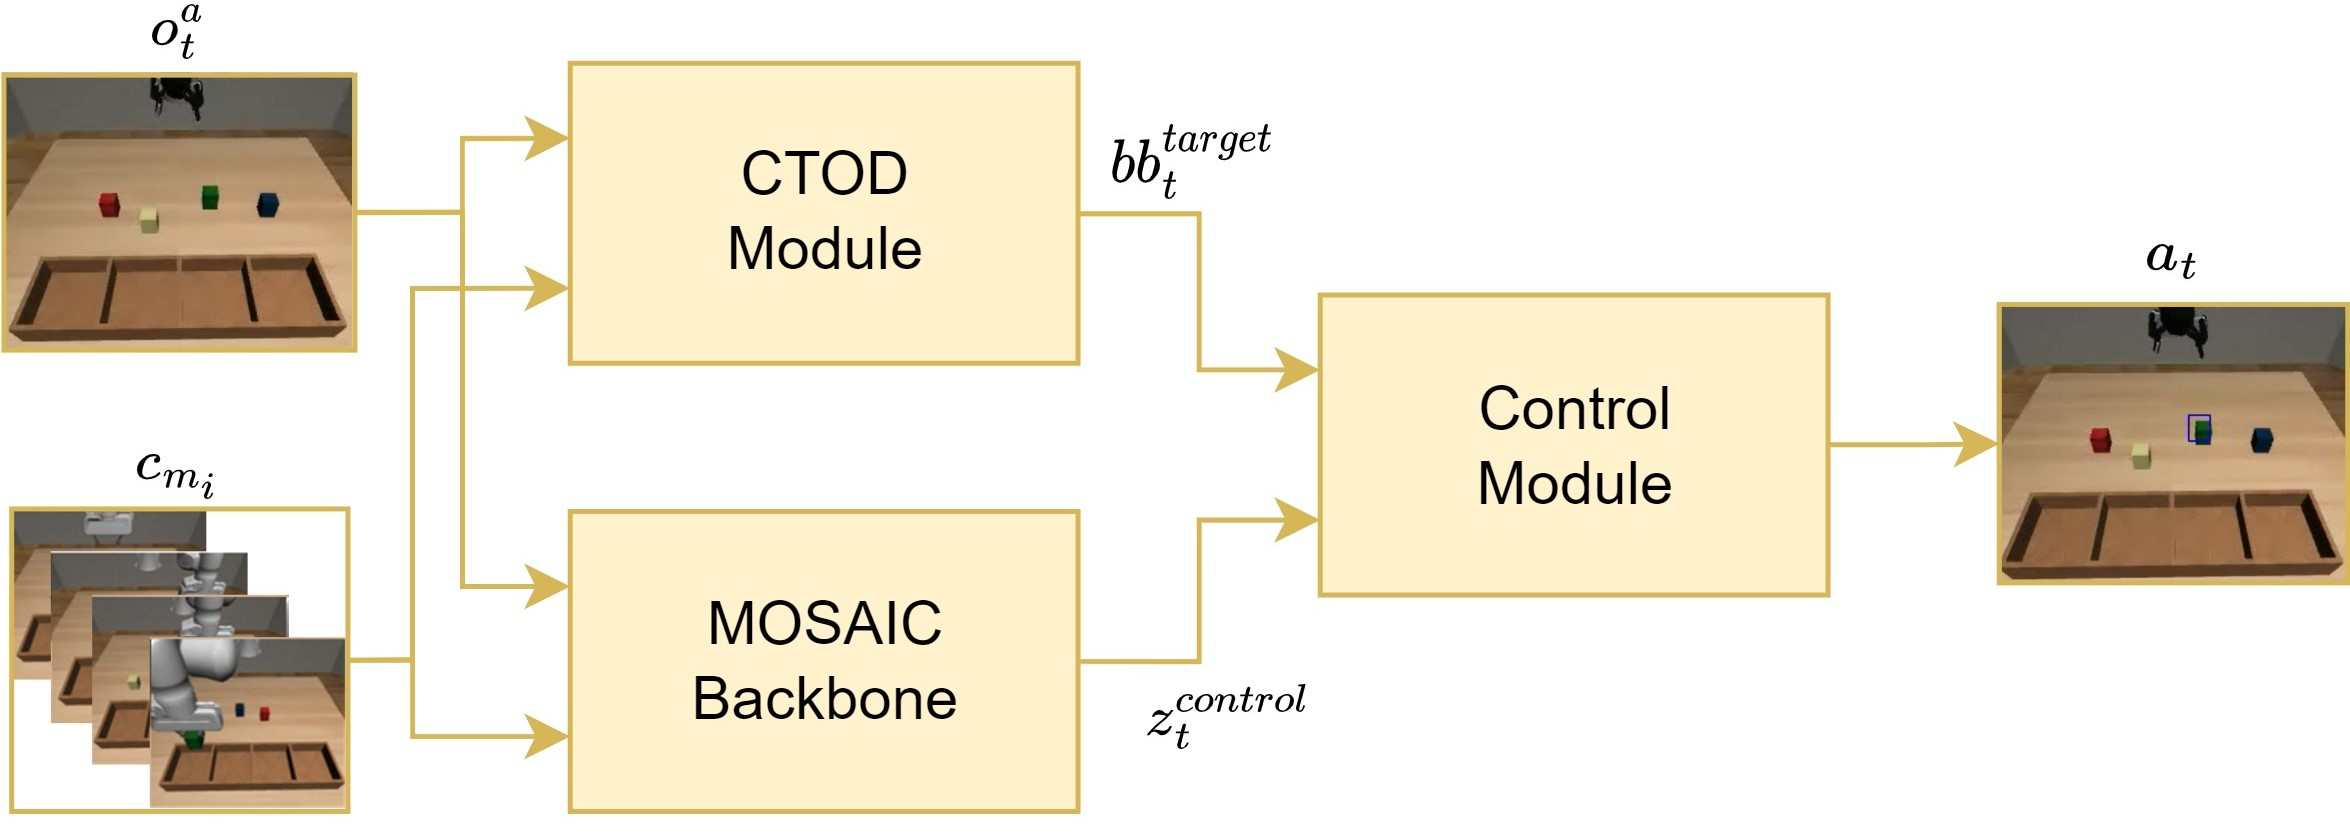
\includegraphics[width=0.9\textwidth]{figures/images/ch3/single_control_module.jpg}
    \caption{Proposed Single-Control Module Architecture. In contrast to the general architecture described in Figure \ref{fig:end_to_end_vs_modular}, the Command Analysis module is replaced by the CTOD module, which generates the bounding box related to the target object. The chosen backbone is the MOSAIC architecture \cite{mandi2022towards_more_generalizable_one_shot}. The control module is now informed by both low-level positional information ($bb^{target}_{t}$) and a control-oriented embedding ($z^{control}_{t}$), enabling it to make more informed decisions.}
    \label{fig:single_control_module}
\end{figure}


\subsection{Double control modules}
\label{sec:ocpl_architecture_dcm}
Regarding the architecture composed of multiple control modules, the discussion must begin with the key observation that the tasks considered can be roughly divided into two phases. The first is generally a \textit{reaching phase}, where the robot must reach a target location. The second phase varies based on the task: placing for Pick-Place, assembly for Nut-Assembly, stacking for Stack-Block, and pushing for Press-Button. Based on this, a dual control module architecture is proposed, with each control module trained to learn the primitive associated with each phase. The rationale behind this approach is that training modules specifically for simpler atomic primitives can result in a more robust and reliable control system.

Figure \ref{fig:double_control_module} illustrates the overall architecture. The main difference can be observed in the bounding boxes received by the control modules. Specifically, the MOSAIC Backbone generates the control embedding $z^{control}_t$, as before. However, the Command Analysis Module, now referred to as the COD Module, generates both the bounding box for the target object, $bb^{target}_t$, and the bounding box for the final placing position, $bb^{place}_t$. 

The $bb^{target}_t$ is provided as input to the \textit{Reaching Control} module, while the $bb^{place}_t$ is supplied to the \textit{Placing Control} module. 

Additionally, each control module operates based on an enabling signal $s^{en}$, which is set to 1 at the beginning of the rollout and remains active until the Reaching Control module generates its first prediction for the closing command. After this point, $s^{en}$ is set to 0, and control is transferred to the Placing Control module.    
\begin{figure}[t]
    \centering
    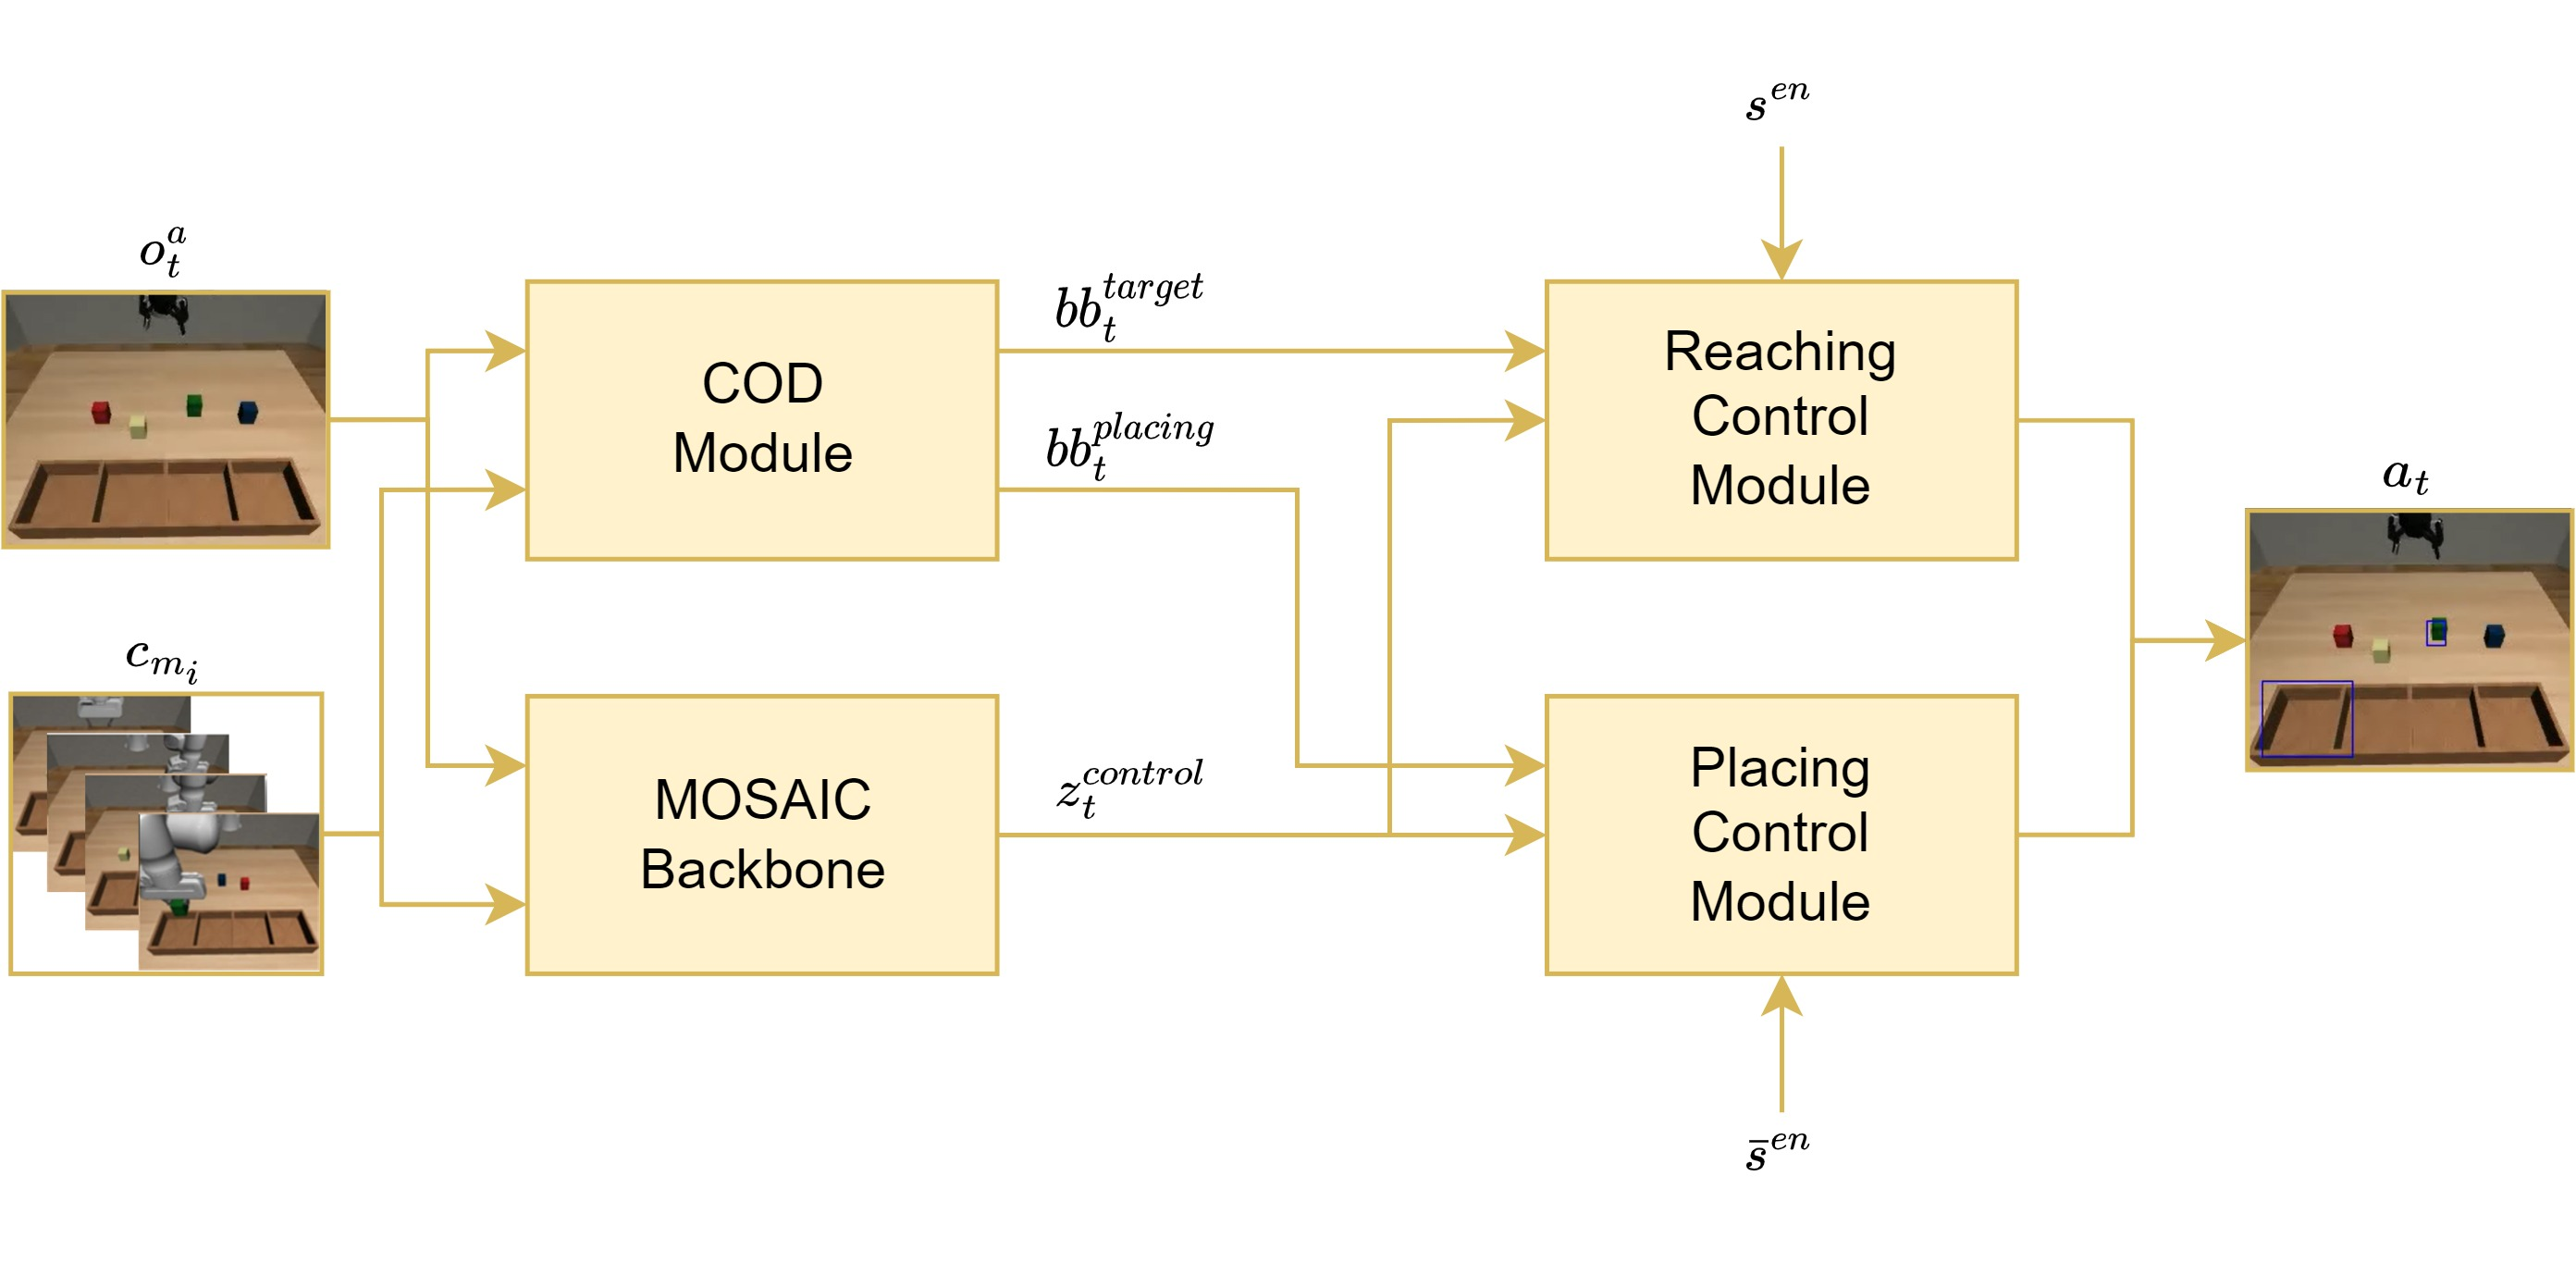
\includegraphics[width=0.9\textwidth]{figures/images/ch3/double_control_module.jpg}
    \caption{Proposed Double-Control Module Architecture. In this architecture, the Control Module is split into two distinct modules, each responsible for learning a specific primitive: the \textit{reaching} primitive and the \textit{placing} primitive. The first module takes as input the bounding box corresponding to the target object ($bb^{target}_{t}$), while the second module receives the bounding box related to the final placing location ($bb^{placing}_{t}$). This separation allows for specialized control during both the reaching and placing phases.}
    \label{fig:double_control_module}
\end{figure}

% \smalltodo{add figure}
\section{Experimental results}
\label{sec:ocpl_experimental}

In this section, the performed experiments are going to be described. Specifically, in  
Section~\ref{sec:ocpl_dataset} the dataset used for training procedure will be described. Section~\ref{sec:ocpl_results} will report the obtained results.
\begin{figure}[t]
    \centering
    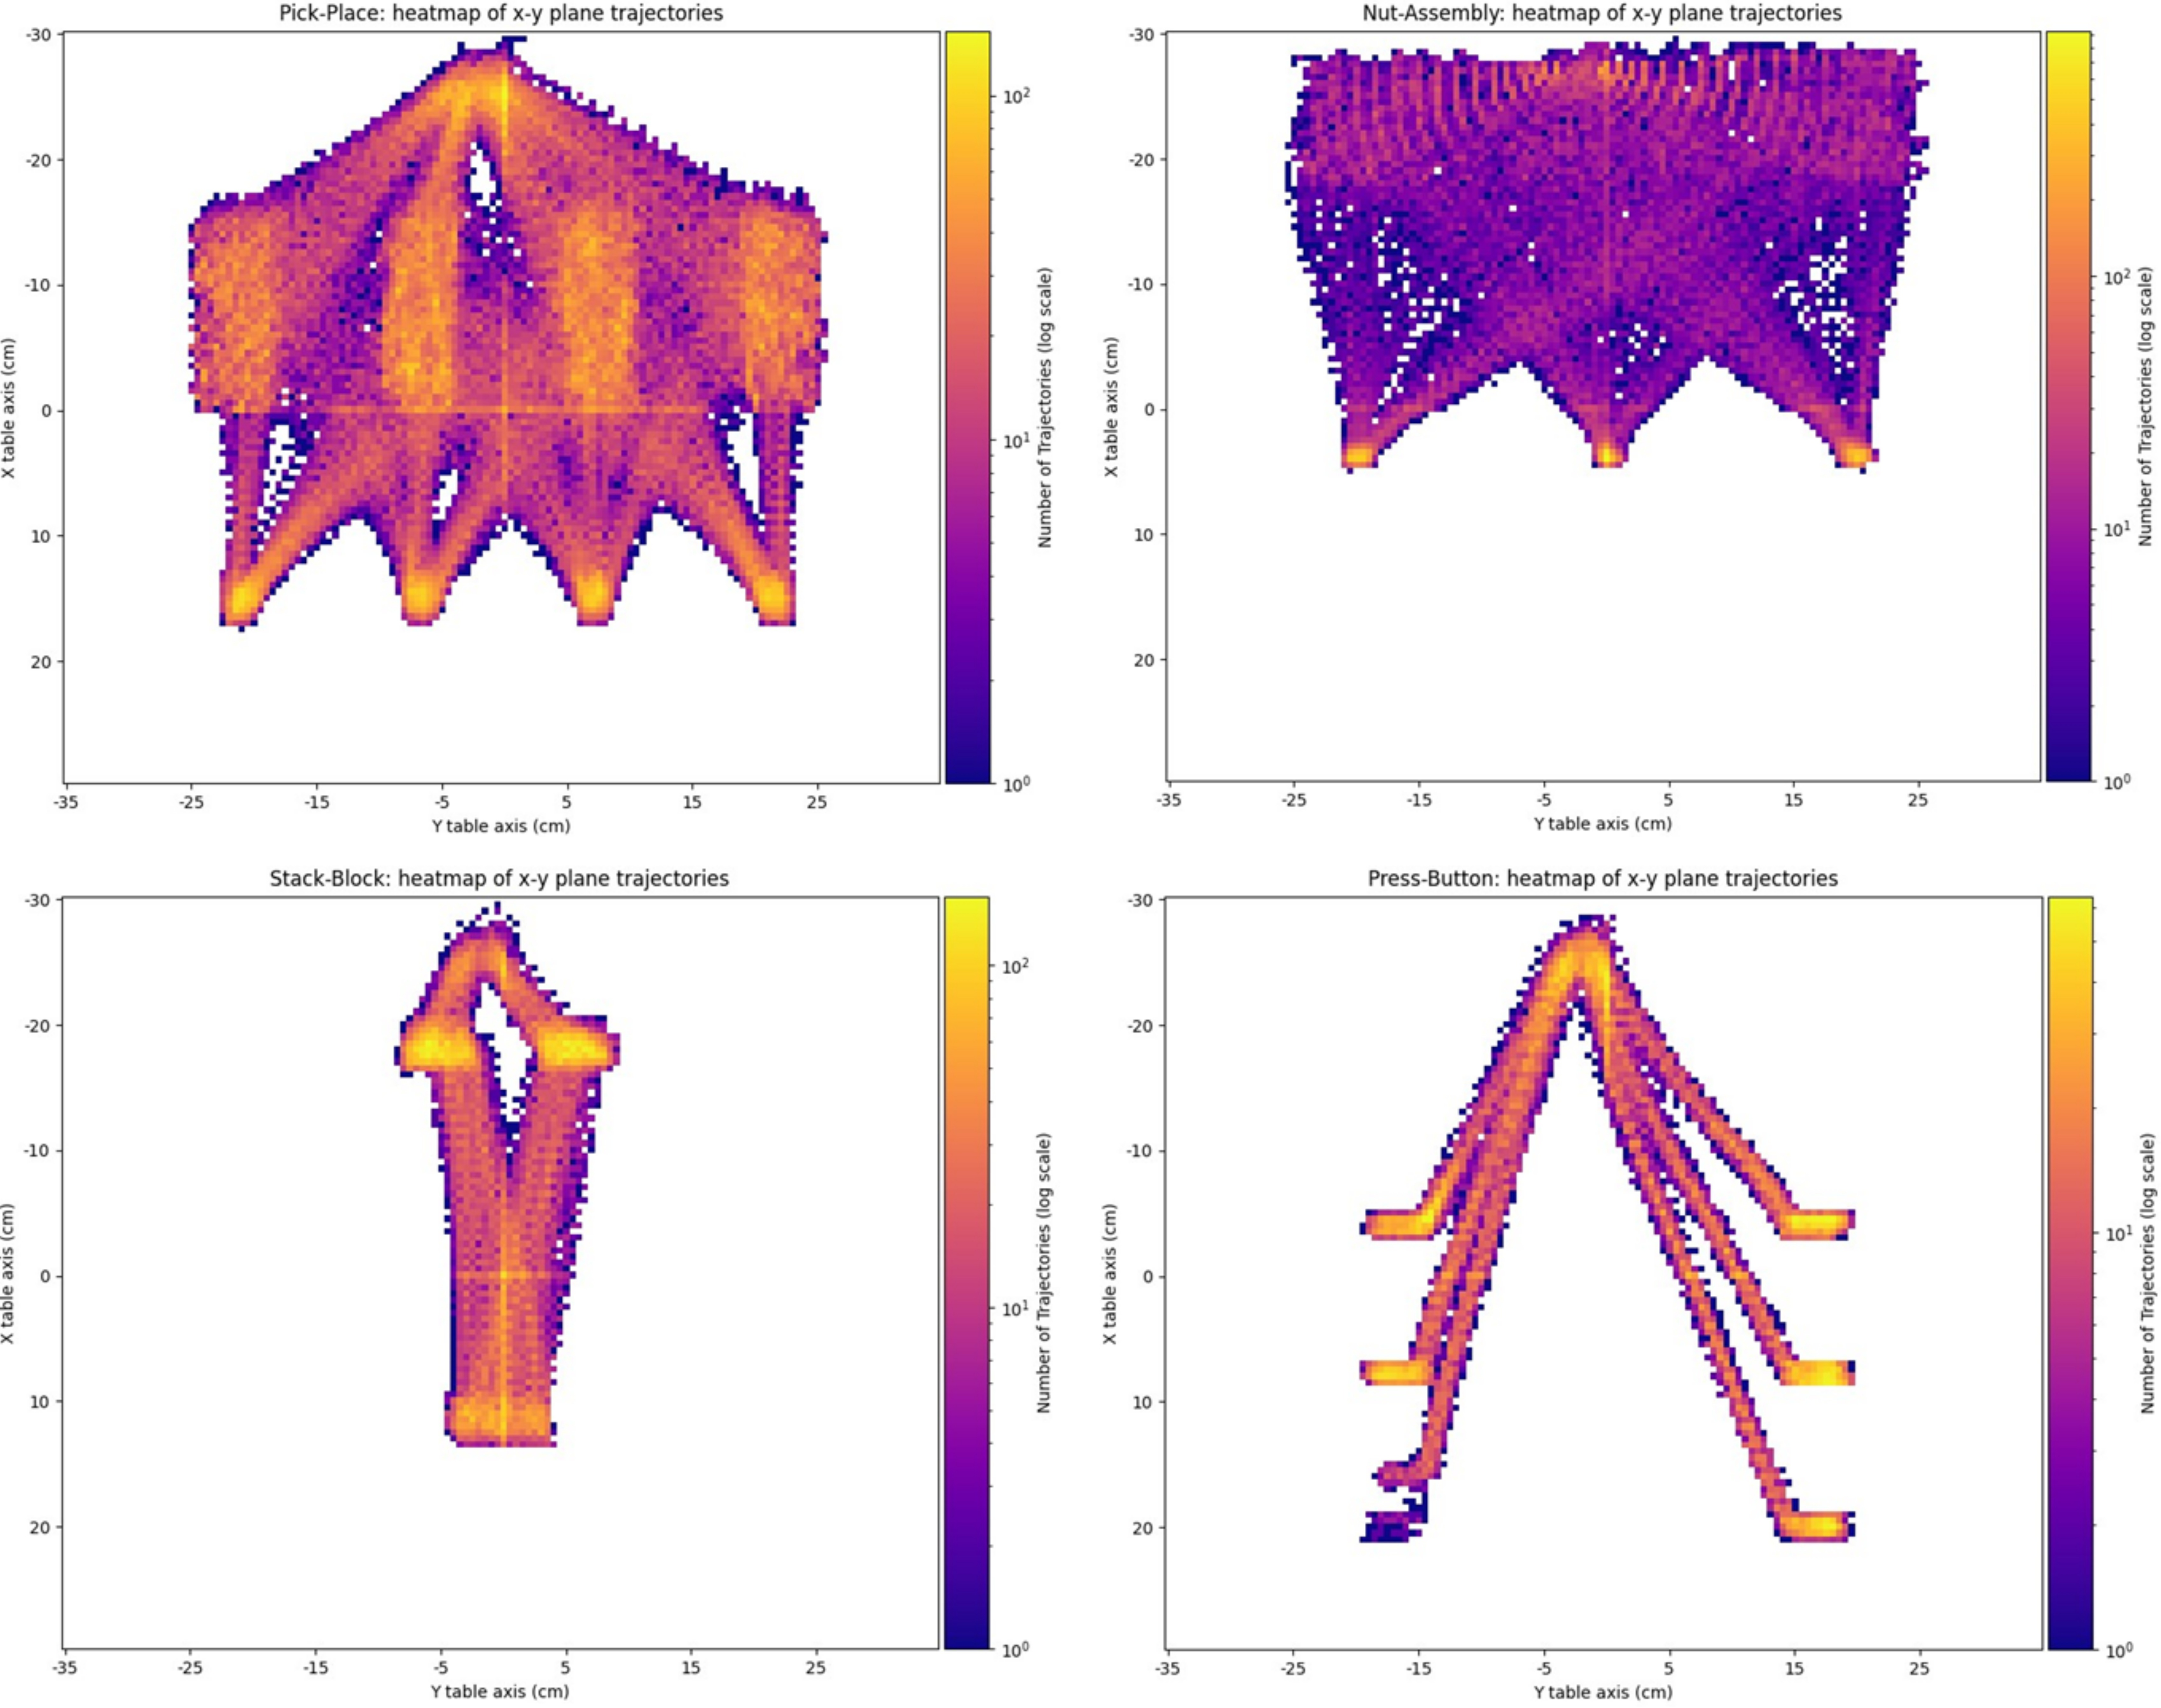
\includegraphics[width=1.0\textwidth]{figures/images/ch3/dataset_distribution.jpg}
    \caption{The distribution of trajectories for the different tasks along the x-y axis of the table workspace.}
    \label{fig:dataset_distribution}
\end{figure}

% The distribution of trajectories for the different tasks along the x-y axis of the table workspace. Each plot represents a density map illustrating the frequency with which the robot's end-effector passed through specific points across all variations and trajectories.
%  The tasks are organized as follows: (Top-Left) Pick-Place, (Top-Right) Nut-Assembly, (Bottom-Left) Stack-Block, and (Bottom-Right) Press-Button.

\subsection{Dataset}
\label{sec:ocpl_dataset}
The dataset used for training the control architectures is described in this section. It consists of the same tasks outlined in Section \ref{sec:cod_dataset}, following the same collection procedure. For each task variation, 100 trajectories were collected for both the agent and the demonstrator. Each trajectory presents a novel object configuration, according to the rules defined in Section \ref{sec:cod_dataset}.

In this section, the dataset is analyzed in terms of the distribution of the action space, in order to highlight the challenges from a control perspective.

Figure \ref{fig:dataset_distribution} illustrates the distribution of the trajectories followed by the robot. Each plot represents a density map illustrating the frequency with which the robot's end-effector passed through specific points across all variations and trajectories, specifically along the $x$ and $y$ axis. Notably, the use of a simulated environment enables complete coverage of the workspace. This particular aspect of the workspace coverage will be further discussed in Chapter \ref{ch:real_world_application} where the real-world system will be discussed.


% \smalltodo{Add figure here.}

Moreover, each task exhibits a \textbf{multi-modal behavior}. This is evident across different variations, as the final placing position changes with each variation. Additionally, during the reaching phase, the robot traverses almost all possible locations within the working area.

It is important to note that, for a given task, the trajectories exhibit significant variation in length. Specifically, for the Pick-Place task, the average trajectory length is \textbf{$71.21 \pm 7.69$} frames. In the Nut-Assembly task, the average length is \textbf{$62.24 \pm 7.47$} frames, while for the Stack-Block task, the average is \textbf{$63.07 \pm 1.51$} frames. Finally, in the Press-Button task, the average trajectory length is\textbf{ $40.45 \pm 8.17$} frames. 

This variability poses a challenge, as the likelihood of errors increases with task progression, and compounding errors become more pronounced over time. Additionally, this multi-modal behavior complicates the learning process. The dataset lacks any prior distribution (i.e., the robot does not consistently approach the target object from the same direction), making it challenging for the architecture to identify and leverage consistent patterns during training.

\subsection{Results}
\label{sec:ocpl_results}
This section presents the obtained results, divided into two main blocks. The first block (Section~\ref{sec:ocpl_results_scm}) discusses the results of the method described in Section\ref{sec:ocpl_architecture_scm}. The second block (Section~\ref{sec:ocpl_results_dcm}) covers the results of the method described in \ref{sec:ocpl_architecture_dcm}. For each method, results are reported for two different scenarios: first, where the method is trained in a single-task multi-variation scenario; and second, where the method is trained in a multi-task multi-variation scenario.

The tests are conducted following the procedure outlined in Section \ref{sec:cod_results}. For each variation, 10 independent runs are performed, each with a novel initial objects configuration. This approach assesses the system robustness with respect to different initial state configurations. Additionally, each set of 10 rollouts is repeated three times to evaluate the overall robustness and consistency of the model.

Various evaluation metrics are considered, either generally defined for each task or task-specific. The general metrics include:

\begin{itemize}
    \item \textit{Reaching}: The ratio of successful attempts where the robot reaches the target object across all rollouts.
    \item \textit{Picking}: The ratio of successful attempts where the robot picks the correct object across all rollouts.
    \item \textit{Success}: The ratio of successful task completions across all rollouts.
    \item \textit{Reaching Wrong}: The ratio of instances where the robot reaches an object other than the target across all rollouts.
    \item \textit{Picking Wrong}: The ratio of instances where the robot picks the wrong object across all rollouts.
    \item \textit{Success with Wrong Object}: The ratio of task completions where the robot manipulates the wrong object.
\end{itemize}

Task-specific metrics, particularly for tasks like Pick-Place and Nut-Assembly, include the 
\textit{Place Wrong with Correct Object} metric, which captures the number of times the robot places the correct object in the wrong position.
% \begin{itemize}
%     \item \textit{Place Wrong with Wrong Object}: The number of times the robot completes the task by placing the wrong object in the wrong position.
%     \item \textit{Place Wrong with Correct Object}: The number of times the robot completes the task by placing the correct object in the wrong position.
% \end{itemize}

These metrics provide a comprehensive evaluation of the robot performance, capturing all major error cases and giving a full picture of its behavior.

\subsubsection{Single control module}
In this section the results obtained with the architecture composed of a Single Control Module will be described. As in Chapter \ref{ch:cod}, there are two testing scenarios, the first one trained with a single-task  multi-variation scenario, while the second one with a multi-task multi-variation setting, with an increasing level of complexity.
\label{sec:ocpl_results_scm}
\paragraph*{Single-task multi-variation scenario}\mbox{}\\

The discussion of the results begins with the single-task multi-variation scenario, focusing on the baseline methods TOSIL \cite{dasari2021transformers_one_shot} and MOSAIC \cite{mandi2022towards_more_generalizable_one_shot}. Specifically, Table \ref{table:occp_single_task_baseline_res} presents the performance of these baseline methods. 
% \usepackage{makecell}
% \usepackage{graphicx}
% \usepackage{multirow}
% \usepackage{hhline}


\begin{table}[t]
    \centering
    % \refstepcounter{table}
    \label{table:occp_single_task_baseline_res}
    \caption{The single-task performance of the baseline methods, TOSIL \cite{dasari2021transformers_one_shot} and MOSAIC \cite{mandi2022towards_more_generalizable_one_shot}, was evaluated. For each model, additional tests were conducted by generating the first 2 steps and 10 steps using the hand-written controller.}
    \resizebox{\linewidth}{!}{%
    \begin{tabular}{|c|c|c|c|c|c|c|c|c|} 
    \hline
    \textbf{Task} & \textbf{Model} & \textbf{GT Action} & \begin{tabular}[c]{@{}c@{}}\textbf{Reaching}\\{[}\%]\end{tabular} & \begin{tabular}[c]{@{}c@{}}\textbf{Picking}\\{[}\%]\end{tabular} & \begin{tabular}[c]{@{}c@{}}\textbf{Success}\\{[}\%]\end{tabular} & \begin{tabular}[c]{@{}c@{}}\textbf{Reaching} \\\textbf{Wrong}~\\{[}\%]\end{tabular} & \begin{tabular}[c]{@{}c@{}}\textbf{Picking}\\\textbf{Wrong}\\{[}\%]\end{tabular} & \begin{tabular}[c]{@{}c@{}}\textbf{Success with}\\\textbf{Wrong Object}\\{[}\%]\end{tabular} \\ 
    \hhline{|=========|}
    \multirow{6}{*}{\rotatebox[origin=c]{90}{Pick-Place}} & \multirow{3}{*}{MOSAIC} & 0 & 62.90$\pm$0.95 & 62.08$\pm$0.95 & 58.75$\pm$1.87 & 36.67$\pm$0.95 & 36.67$\pm$0.95 & \textbf{37.71$\pm$0.72} \\ 
    \cline{3-9}
     & & 2 & 89.17$\pm$1.30 & 88.12$\pm$
      0.62 & 84.17$\pm$
      1.57 & 11.25$\pm$
      1.25 & 11.25$\pm$
      1.25 & 11.46$\pm$
      1.30 \\ 
    \cline{3-9}
     &  & 10 & 99.79$\pm$0.36 & 98.54$\pm$0.72 & \textbf{95.63$\pm$0.63} & 1.25$\pm$0.63 & 1.25$\pm$0.63 & 0.41$\pm$0.36 \\ 
    \cline{2-9}
     & \multirow{3}{*}{TOSIL} & 0 & 33.12$\pm$1.08 & 27.92$\pm$
      0.72 & 26.87$\pm$
      0.62 & 63.96$\pm$
      2.36 & 63.75$\pm$
      2.72 & \textbf{66.04$\pm$1.57} \\ 
    \cline{3-9}
     & & 2 & 69.17$\pm$1.30 & 60.83$\pm$2.52 & 59.38$\pm$2.17 & 29.17$\pm$0.95 & 28.96$\pm$1.30 & 30.83$\pm$2.20 \\ 
    \cline{3-9}
     &  & 10 & 98.58$\pm$0.36 & 92.71$\pm$
      1.44 & \textbf{90.00$\pm$1.08} & 2.70$\pm$
      1.30 & 2.70$\pm$
      1.30 & 1.25$\pm$
      0.62 \\ 
    \hhline{|=========|}
    \multirow{6}{*}{\rotatebox[origin=c]{90}{Nut-Assembly}} & \multirow{3}{*}{MOSAIC} & 0 & 38.89$\pm$1.11 & 36.67$\pm$1.11 & 33.33$\pm$1.11 & 59.26$\pm$1.69 & 55.93$\pm$1.69 & \textbf{51.48$\pm$2.31} \\ 
    \cline{3-9}
     & & 2 & 85.19$\pm$
      4.49 & 83.33$\pm$
      5.09 & 78.89$\pm$
      4.01 & 13.33$\pm$
      4.84 & 11.85$\pm$
      2.31 & 11.11$\pm$
      2.22 \\ 
    \cline{3-9}
     &  & 10 & 100.00$\pm$100.00 & 99.26$\pm$1.28 & \textbf{90.74$\pm$2.79} & 0.00$\pm$0.00 & 0.00$\pm$0.00 & 0.00$\pm$0.00 \\ 
    \cline{2-9}
     & \multirow{3}{*}{TOSIL} & 0 & 36.30$\pm$
      1.28 & 35.19$\pm$
      2.31 & 31.11$\pm$
      1.92 & 63.33$\pm$
      1.11 & 62.59$\pm$
      1.28 & \textbf{56.30$\pm$3.57} \\ 
    \cline{3-9}
     & & 2 & 83.33$\pm$2.22 & 82.96$\pm$2.31 & 77.78$\pm$2.22 & 16.67$\pm$2.22 & 16.67$\pm$2.22 & 14.44$\pm$1.11 \\ 
    \cline{3-9}
     &  & 10 & 100.00$\pm$
      0.00 & 99.26$\pm$
      1.28 & \textbf{88.89$\pm$2.22} & 0.00$\pm$
      0.00 & 0.00$\pm$
      0.00 & 0.00$\pm$
      0.00 \\ 
    \hhline{|=========|}
    \multirow{6}{*}{\rotatebox[origin=c]{90}{Stack-Block}} & \multirow{3}{*}{MOSAIC} & 0 & 60.56$\pm$0.96 & 60.56$\pm$0.96 & 53.33$\pm$1.66 & 39.44$\pm$0.96 & 39.44$\pm$0.96 & \textbf{36.11$\pm$0.96} \\ 
    \cline{3-9}
     & & 2 & 91.11$\pm$
      0.96 & 90.56$\pm$
      0.96 & 73.89$\pm$
      4.19 & 7.70$\pm$
      0.96 & 7.70$\pm$
      0.96 & 7.20$\pm$
      0.96 \\ 
    \cline{3-9}
     &  & 10 & 100.00$\pm$0.00 & 99.44$\pm$0.96 & \textbf{77.78$\pm$1.92} & 0.00$\pm$0.00 & 0.00$\pm$0.00 & 0.00$\pm$0.00 \\ 
    \cline{2-9}
     & \multirow{3}{*}{TOSIL} & 0 & 69.44$\pm$
      0.96 & 60.00$\pm$
      0.16 & 48.89$\pm$
      2.54 & 42.78$\pm$
      0.96 & 42.78$\pm$
      0.96 & \textbf{41.67$\pm$1.66} \\ 
    \cline{3-9}
     & & 2 & 90.56$\pm$0.96 & 87.78$\pm$0.96 & 79.44$\pm$1.92 & 12.22$\pm$0.96 & 11.67$\pm$0.00 & 11.67$\pm$0.00 \\ 
    \cline{3-9}
     &  & 10 & 100.00$\pm$
      0.00 & 99.44$\pm$
      0.96 & \textbf{88.89$\pm$1.92} & 1.66$\pm$
      1.66 & 1.11$\pm$
      0.96 & 0.00$\pm$
      0.00 \\ 
    \hhline{|=========|}
    \multirow{6}{*}{\rotatebox[origin=c]{90}{Press-Button}} & \multirow{3}{*}{MOSAIC} & 0 & 100.00$\pm$0.00 & - & \textbf{100.00$\pm$0.00} & 0.00$\pm$0.00 & - & 0.00$\pm$0.00 \\ 
    \cline{3-9}
     & & 2 & 100.00$\pm$
      0.00 & - & 100.00,
      0.00 & 0.00$\pm$
      0.00 & - & 0.00$\pm$
      0.00 \\ 
    \cline{3-9}
     &  & 10 & 100.00$\pm$0.00 & - & 100.00$\pm$0.00 & 0.00$\pm$0.00 & - & 0.00$\pm$0.00 \\ 
    \cline{2-9}
     & \multirow{3}{*}{TOSIL} & 0 & 83.33$\pm$
      1.66 & - & \textbf{83.33$\pm$1.66} & 17.78$\pm$
      1.93 & - & 16.67$\pm$
      1.67 \\ 
    \cline{3-9}
     & & 2 & 80.56$\pm$1.92 & - & 80.56$\pm$1.92 & 20.00$\pm$2.88 & - & 18.33$\pm$2.89 \\ 
    \cline{3-9}
     &  & 10 & 92.22$\pm$
      0.96 & - & 81.67$\pm$
      3.33 & 9.44$\pm$
      0.96 & - & 9.44$\pm$
      0.96 \\
    \hline
    \end{tabular}
    }
    \end{table}

As observed, both baseline methods suffer from the issue of \textbf{target-object misidentification}. This is evident from the \textit{Success with Wrong Object} column, where the success rate involving wrong objects is significant. Figure \ref{fig:baseline_pick_place_error} provides an example of a pick-and-place rollout in which the task is technically completed, but the wrong object is manipulated.
\begin{figure}[t]
    \centering
    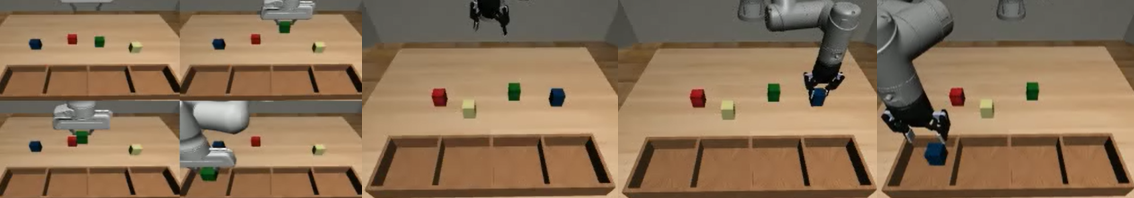
\includegraphics[width=1.0\textwidth]{figures/images/baseline_pick_place_error/pick_place_trj.png}
    \caption{Example of task rollout with incorrect object manipulation. In this scenario, the robot successfully completes the task by placing an object in the first bin. However, instead of manipulating the correct object (the green box), the robot mistakenly picks up the blue box. This illustrates a situation where the robot executes the task's final action correctly but selects the wrong object during manipulation.}
    \label{fig:baseline_pick_place_error}
\end{figure}

% \smalltodo{Add Figure}

To investigate the cause of these errors, test rollouts were conducted using the first 2 and 10 actions generated by a hand-written policy with access to ground-state information. Notably, the success rate improves significantly by applying just 2 ground-truth actions. This observation supports the hypothesis outlined in Section \ref{sec:ocpl_problem}, suggesting that the end-to-end architecture trained with an action-centric loss produces a suboptimal embedding $z$ for the cognitive task. Specifically, the embedding does not adequately inform the control policy about the correct position of the target object.

Based on this consideration, the thesis proposal to inform the control module with both a low-level positional information (e.g., the bouding-box of the target object) and a control embedding generated by the MOSAIC-backbone has been tested. During this test, two models variations have been considered, the first named \textit{MOSAIC-GT-BB} is basically the MOSAIC model, with the Control Module that receives in input the control-embedding $z^{control}$ and the ground-truth bouding-box. The second, named \textit{MOSAIC-CTOD} is the architecture described in Section \ref{sec:ocpl_architecture_scm}.

\begin{table}[t]
  \centering
  \caption{The single-task performance of the proposed MOSAIC-CTOD module is compared to the MOSAIC and MOSAIC-GT-BB baselines. MOSAIC-GT-BB refers to the MOSAIC model, where the Control Module receives the ground-truth target bounding box as input.}
  \label{table:ctod_single_task}
  \resizebox{\linewidth}{!}{%
  \begin{tabular}{|c|c|c|c|c|c|c|c|} 
  \hline
  \textbf{Task} & \textbf{Method} & \begin{tabular}[c]{@{}c@{}}\textbf{Reaching}\\{[}\%]\end{tabular} & \begin{tabular}[c]{@{}c@{}}\textbf{Picking}\\{[}\%]\end{tabular} & \begin{tabular}[c]{@{}c@{}}\textbf{Success}\\{[}\%]\end{tabular} & \begin{tabular}[c]{@{}c@{}}\textbf{Reaching }\\\textbf{Wrong~}\\{[}\%]\end{tabular} & \begin{tabular}[c]{@{}c@{}}\textbf{Picking}\\\textbf{Wrong}\\{[}\%]\end{tabular} & \begin{tabular}[c]{@{}c@{}}\textbf{Success with}\\\textbf{Wrong Object}\\{[}\%]\end{tabular} \\ 
  \hhline{|========|}
  \multirow{3}{*}{Pick-Place} & MOSAIC & 62.90$\pm$0.95 & 62.08$\pm$0.95 & 58.75$\pm$1.87 & 36.67$\pm$0.95 & 36.67$\pm$0.95 & 37.71$\pm$0.72 \\ 
  \cline{2-8}
   & MOSAIC-GT-BB & 100.00$\pm$   0.00 & 97.71$\pm$   0.72 & 76.46$\pm$   3.20 & 0.00$\pm$   0.00 & 0.00$\pm$   0.00 & 0.00$\pm$   0.00 \\ 
  \cline{2-8}
   & MOSAIC-CTOD & 98.12$\pm$0.62 & 91.88$\pm$4.88 & \textbf{77.11$\pm$5.60} & 1.04$\pm$0.36 & 1.04$\pm$0.36 & 1.04$\pm$0.36 \\ 
  \hhline{|========|}
  \multirow{3}{*}{Nut-Assembly} & MOSAIC & 38.89$\pm$1.11 & 36.67$\pm$1.11 & 33.33$\pm$1.11 & 59.26$\pm$1.69 & 55.93$\pm$1.69 & 51.48$\pm$2.31 \\ 
  \cline{2-8}
   & MOSAIC-GT-BB & 100.00$\pm$   0.00 & 98.89$\pm$   1.11 & \textbf{70.37$\pm$1.69} & 0.00$\pm$   0.00 & 0.00$\pm$   0.00 & 0.00$\pm$   0.00 \\ 
  \cline{2-8}
   & MOSAIC-CTOD & 98.89$\pm$1.11 & 97.41$\pm$2.31 & 64.07$\pm$0.64 & 0.00$\pm$0.00 & 0.00$\pm$0.00 & 0.00$\pm$0.00 \\ 
  \hhline{|========|}
  \multirow{3}{*}{Stack-Block} & MOSAIC & 60.56$\pm$0.96 & 60.56$\pm$0.96 & 53.33$\pm$1.66 & 39.44$\pm$0.96 & 39.44$\pm$0.96 & 36.11$\pm$0.96 \\ 
  \cline{2-8}
   & MOSAIC-GT-BB & 100.00$\pm$   0.00 & 99.44$\pm$   0.96 & 90.00$\pm$   2.89 & 0.00$\pm$   0.00 & 0.00$\pm$   0.00 & 0.00$\pm$   0.00 \\ 
  \cline{2-8}
   & MOSAIC-CTOD & 100.00$\pm$0.00 & 100.00$\pm$0.00 & \textbf{91.67$\pm$2.88} & 0.00$\pm$0.00 & 0.00$\pm$0.00 & 0.00$\pm$0.00 \\ 
  \hhline{|========|}
  \multirow{3}{*}{Press-Button} & MOSAIC & 100.00$\pm$0.00 & - & \textbf{100.00$\pm$0.00} & 0.00$\pm$0.00 & - & 0.00$\pm$0.00 \\ 
  \cline{2-8}
   & MOSAIC-GT-BB & 92.22$\pm$   2.54 & - & 90.56$\pm$   1.92 & 3.88$\pm$   0.96 & - & 3.88$\pm$   0.96 \\ 
  \cline{2-8}
   & MOSAIC-CTOD & 97.22$\pm$1.92 & - & 95.56$\pm$1.92 & 2.77$\pm$0.96 & - & 2.77$\pm$0.96 \\
  \hline
  \end{tabular}
  }
  \end{table}
The results are summarized in Table \ref{table:ctod_single_task_performance}. Several key observations can be made from these findings. For tasks involving multiple similar objects that change positions across different demonstrations (such as Pick-Place, Nut-Assembly, and Stack-Block), the use of positional information significantly enhances the system robustness. This enables the robot to consistently reach the target object and improves the overall success rate.

In contrast, for the Press-Button task, while the MOSAIC-CTOD method achieves a high success rate (95.56\% on average), it does not overcome the baseline method, which consistently solves the task with a 100\% success rate. This limitation arises because, once the button is reached, the positional information provides no further guidance on how to complete the task. Consequently, the robot often gets stuck near the button, failing to execute the pushing action (Figure \ref{fig:button_ctod_error}).
\begin{figure}[t]
    \centering
    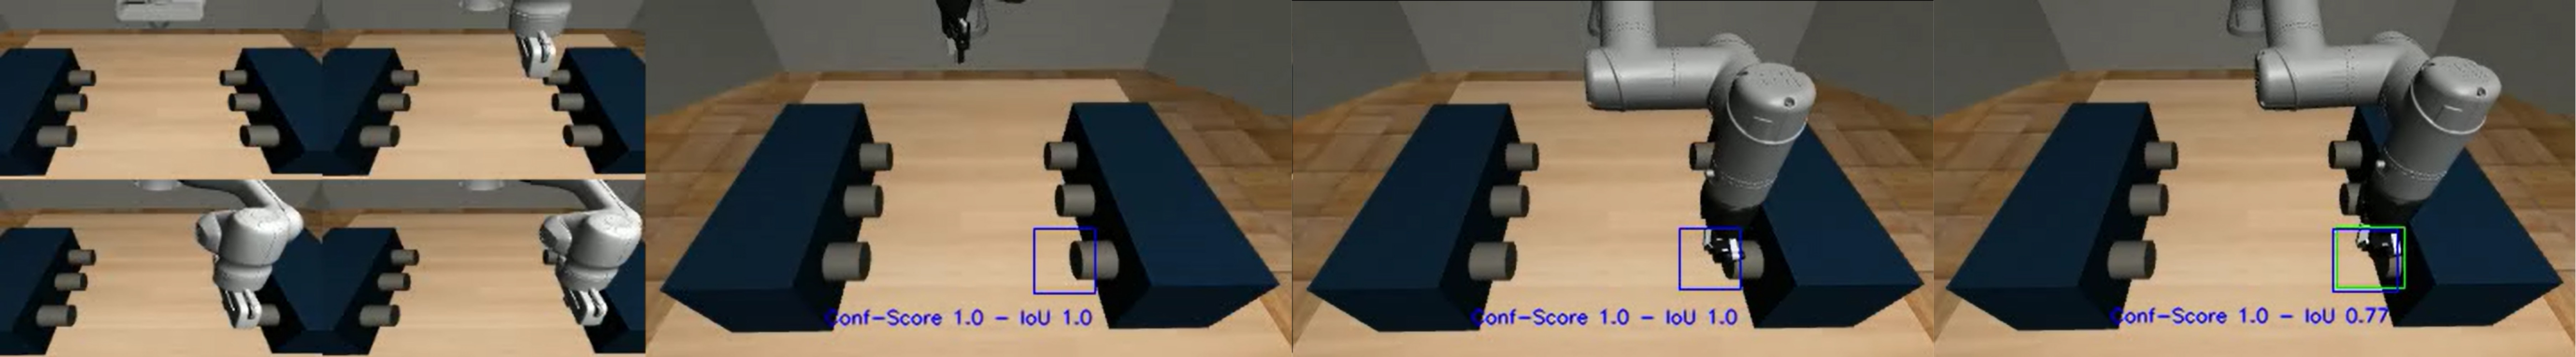
\includegraphics[width=1.0\textwidth]{figures/images/ch3/button_error.jpg}
    \caption{Example of unsuccessful Press-Button rollout. In this scenario, the robot successfully reaches the target button using the predicted bounding box (blue). However, due to instability in predictions during the pushing phase, the robot is unable to complete the pressing action, resulting in an unsuccessful task execution.}
    \label{fig:button_ctod_error}
\end{figure}

% \smalltodo{Add Figure}

Furthermore, the inclusion of positional information introduces a novel type of error. Specifically, since the robot behavior is conditioned by the bounding box, any error in its prediction can cause the robot to move incorrectly (Figure \ref{fig:error_propagation}). This error is significant, as in the Pick-Place task, the metric ``Place Wrong with Correct Object" reaches 11.25\%, and for the Nut-Assembly task, the same metric averages 22.22\%.
\begin{figure}[t]
    \centering
    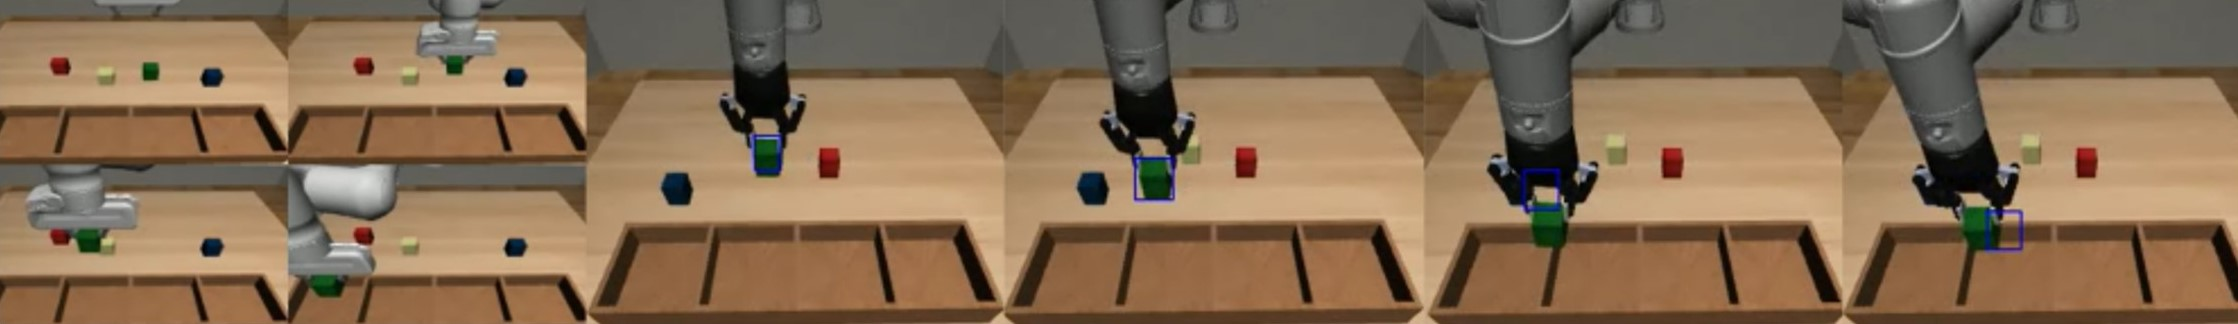
\includegraphics[width=1.0\textwidth]{figures/images/ch3/error_propagation.jpg}
    \caption{Example of unsuccessful Pick-Place rollout. In this case, the robot fails to complete the task due to errors in the bounding box predictions. These inaccuracies cause the robot to move in the wrong direction, leading to an unsuccessful execution of the task.}
    \label{fig:error_propagation}
\end{figure}


To address this issue, the Double-Control Module architecture has been proposed (Section \ref{sec:ocpl_architecture_dcm}), with the corresponding results presented in Section \ref{sec:ocpl_results_dcm}.

\paragraph*{Multi-task multi-variation scenario}\mbox{}\\
As in the previous paragraph, an evaluation of the two baseline methods was also conducted in the multi-task setting. The results are summarized in Table \ref{table:occp_multi_task_baseline_res}. The same general trends and behaviors observed in the single-task scenario are present here as well. Specifically, both baselines demonstrate the ability to produce reasonable trajectories that allow the robot to complete the task, though they manipulate the wrong object.

Furthermore, when comparing the results from Table \ref{table:occp_single_task_baseline_res} with those in Table \ref{table:occp_multi_task_baseline_res}, it is evident that the success rate decreases across all methods in the more complex multi-task setting. This highlights a potential issue with task balancing during the learning process.
% \usepackage{makecell}
% \usepackage{graphicx}
% \usepackage{multirow}
% \usepackage{hhline}


\begin{table}[t]
  \centering
  \caption{The multi-task performance of the baseline methods, TOSIL \cite{dasari2021transformers_one_shot} and MOSAIC \cite{mandi2022towards_more_generalizable_one_shot}, was evaluated. For each model, additional tests were conducted by generating the first 2 steps and 10 steps using the hand-written controller.}
  \label{table:occp_multi_task_baseline_res}
  \resizebox{\linewidth}{!}{%
  \begin{tabular}{|c|c|c|c|c|c|c|c|c|} 
  \hline
  \textbf{Task} & \textbf{Model} & \textbf{GT Action} & \begin{tabular}[c]{@{}c@{}}\textbf{Reaching}\\{[}\%]\end{tabular} & \begin{tabular}[c]{@{}c@{}}\textbf{Picking}\\{[}\%]\end{tabular} & \begin{tabular}[c]{@{}c@{}}\textbf{Success}\\{[}\%]\end{tabular} & \begin{tabular}[c]{@{}c@{}}\textbf{Reaching} \\\textbf{Wrong}~\\{[}\%]\end{tabular} & \begin{tabular}[c]{@{}c@{}}\textbf{Picking}\\\textbf{Wrong}\\{[}\%]\end{tabular} & \begin{tabular}[c]{@{}c@{}}\textbf{Success with}\\\textbf{Wrong Object}\\{[}\%]\end{tabular} \\ 
  \hhline{|=========|}
  \multirow{6}{*}{\rotatebox[origin=c]{90}{Pick-Place}} & \multirow{3}{*}{MOSAIC} & 0 & 25.83$\pm$1.30 & 23.96$\pm$0.72 & 22.71$\pm$0.72 & 65.63$\pm$2.87 & 63.96$\pm$1.90 & \textbf{67.92$\pm$1.30} \\ 
  \cline{3-9}
   &  & 2 & 61.04$\pm$2.19 & 58.13$\pm$2.86 & 56.46$\pm$3.14 & 36.04$\pm$1.90 & 35.42$\pm$1.90 & 36.25$\pm$1.08 \\ 
  \cline{3-9}
   &  & 10 & 97.77$\pm$0.36 & 95.00$\pm$0.62 & \textbf{87.50$\pm$1.25} & 2.50$\pm$0.62 & 2.29$\pm$0.95 & 2.29$\pm$0.72 \\ 
  \cline{2-9}
   & \multirow{3}{*}{TOSIL} & 0 & 35.42$\pm$0.72 & 27.08$\pm$1.30 & 26.46$\pm$1.80 & 60.21$\pm$1.57 & 59.58$\pm$1.44 & 59.58$\pm$1.44 \\ 
  \cline{3-9}
   &  & 2 &  &  &  &  &  &  \\ 
  \cline{3-9}
   &  & 10 &  &  &  &  &  &  \\ 
  \hhline{|=========|}
  \multirow{6}{*}{\rotatebox[origin=c]{90}{Stack-Block}} & \multirow{3}{*}{MOSAIC} & 0 & 32.96$\pm$1.28 & 30.74$\pm$2.31 & 28.53$\pm$2.31 & 56.30$\pm$4.49 & 48.15$\pm$4.20 & 41.67$\pm$1.66 \\ 
  \cline{3-9}
   &  & 2 & 76.67$\pm$1.11 & 73.33$\pm$1.92 & 65.56$\pm$4.00 & 19.63$\pm$0.64 & 17.41$\pm$1.28 & 17.04$\pm$1.69 \\ 
  \cline{3-9}
   &  & 10 & 100.00$\pm$0.00 & 97.78$\pm$1.11 & \textbf{82.96$\pm$1.28} & 0.00$\pm$0.00 & 0.00$\pm$0.00 & 0.00$\pm$0.00 \\ 
  \cline{2-9}
   & \multirow{3}{*}{TOSIL} & 0 & 27.78$\pm$2.94 & 24.44$\pm$2.94 & 22.59$\pm$3.57 & 70.37$\pm$2.57 & 67.78$\pm$2.22 & \textbf{64.81$\pm$2.57} \\ 
  \cline{3-9}
   &  & 2 &  &  &  &  &  &  \\ 
  \cline{3-9}
   &  & 10 &  &  &  &  &  &  \\ 
  \hhline{|=========|}
  \multirow{6}{*}{\rotatebox[origin=c]{90}{Nut-Assembly}} & \multirow{3}{*}{MOSAIC} & 0 & 57.78$\pm$1.92 & 57.78$\pm$1.92 & 55.56$\pm$2.54 & 42.22$\pm$1.92 & 42.22$\pm$1.93 & 41.11$\pm$1.67 \\ 
  \cline{3-9}
   &  & 2 & 95.56$\pm$0.96 & 95.56$\pm$0.96 & 89.44$\pm$1.92 & 4.44$\pm$0.96 & 4.44$\pm$0.96 & 4.44$\pm$0.96 \\ 
  \cline{3-9}
   &  & 10 & 100.00$\pm$0.00 & 100.00$\pm$0.00 & \textbf{92.22$\pm$0.96} & 0.00$\pm$0.00 & 0.00$\pm$0.00 & 0.00$\pm$0.00 \\ 
  \cline{2-9}
   & \multirow{3}{*}{TOSIL} & 0 & 54.44$\pm$0.96 & 54.44$\pm$0.96 & 48.89$\pm$0.96 & 46.11$\pm$0.96 & 45.56$\pm$0.96 & \textbf{45.56$\pm$0.96} \\ 
  \cline{3-9}
   &  & 2 &  &  &  &  &  &  \\ 
  \cline{3-9}
   &  & 10 &  &  &  &  &  &  \\ 
  \hhline{|=========|}
  \multirow{6}{*}{\rotatebox[origin=c]{90}{Press-Button}} & \multirow{3}{*}{MOSAIC} & 0 & 78.33$\pm$1.66 & - & 77.22$\pm$2.54 & 22.78$\pm$2.54 & - & 22.78$\pm$2.54 \\ 
  \cline{3-9}
   &  & 2 & 77.22$\pm$0.96 & - & 76.67$\pm$1.67 & 23.33$\pm$1.66 & - & 23.33$\pm$1.66 \\ 
  \cline{3-9}
   &  & 10 & 82.78$\pm$2.54 & - & \textbf{80.00$\pm$3.33} & 20.00$\pm$3.33 & - & 20.00$\pm$3.33 \\ 
  \cline{2-9}
   & \multirow{3}{*}{TOSIL} & 0 & 70.56$\pm$7.52 & - & 60.59$\pm$11.34 & 27.22$\pm$2.47 & - & \textbf{27.22$\pm$2.47} \\ 
  \cline{3-9}
   &  & 2 &  & - &  &  & - &  \\ 
  \cline{3-9}
   &  & 10 &  & - &  &  & - &  \\
  \hline
  \end{tabular}
  }
  \end{table}

After evaluating the baseline, the proposed MOSAIC-CTOD was tested, using the same variations as in the previous section. Table \ref{table:ctod_multi_task} summarizes the results obtained with the inclusion of positional information. Compared to the baseline, a general improvement is observed. However, caution is required when training the system in a multi-task setting. Specifically, when comparing the single-task performance (Table \ref{table:mosaic_ctod_single_task}) to the multi-task performance, there is a noticeable drop in success rates for the same tasks. This decline is particularly evident in the system's ability to execute the ``pick" primitive, especially when the nut object is involved. This observation underscores the importance of incorporating regularization techniques during multi-task learning to manage the varying complexities of different tasks.
% \usepackage{graphicx}
% \usepackage{multirow}
% \usepackage{hhline}


\begin{table}[t]
  \centering
  \caption{The multi-task performance of the proposed MOSAIC-CTOD module is compared to the MOSAIC and MOSAIC-GT-BB baselines. MOSAIC-GT-BB refers to the MOSAIC model, where the Control Module receives the ground-truth target bounding box as input.}
  \label{table:ctod_multi_task}
  \resizebox{\linewidth}{!}{%
  \begin{tabular}{|c|c|c|c|c|c|c|c|} 
  \hline
  \textbf{Task} & \textbf{Method} & \begin{tabular}[c]{@{}c@{}}\textbf{Reaching}\\{[}\%]\end{tabular} & \begin{tabular}[c]{@{}c@{}}\textbf{Picking}\\{[}\%]\end{tabular} & \begin{tabular}[c]{@{}c@{}}\textbf{Success}\\{[}\%]\end{tabular} & \begin{tabular}[c]{@{}c@{}}\textbf{Reaching }\\\textbf{Wrong~}\\{[}\%]\end{tabular} & \begin{tabular}[c]{@{}c@{}}\textbf{Picking}\\\textbf{Wrong}\\{[}\%]\end{tabular} & \begin{tabular}[c]{@{}c@{}}\textbf{Success with}\\\textbf{Wrong Object}\\{[}\%]\end{tabular} \\ 
  \hhline{|========|}
  \multirow{3}{*}{Pick-Place} & MOSAIC & 25.83$\pm$1.30 & 23.96$\pm$0.72 & 22.71$\pm$0.72 & 65.63$\pm$2.87 & 63.96$\pm$1.90 & 67.92$\pm$1.30 \\ 
  \cline{2-8}
   & MOSAIC-GT-BB & 100.00$\pm$0.00 & 89.58$\pm$2.19 & \textbf{58.33$\pm$0.90} & 0.00$\pm$0.00 & 0.00$\pm$0.00 & 0.00$\pm$0.00 \\ 
  \cline{2-8}
   & \begin{tabular}[c]{@{}c@{}}\textit{\textbf{MOSAIC-CTOD}}\\\textit{\textbf{(proposal)}}\end{tabular} & 80.21$\pm$1.44 & 67.50$\pm$0.62 & 53.33$\pm$1.90 & 4.16$\pm$0.71 & 3.54$\pm$0.36 & 0.37$\pm$0.64 \\ 
  \hhline{|========|}
  \multirow{3}{*}{Nut-Assembly} & MOSAIC & 32.96$\pm$1.28 & 30.74$\pm$2.31 & 28.53$\pm$2.31 & 56.30$\pm$4.49 & 48.15$\pm$4.20 & 41.67$\pm$1.66 \\ 
  \cline{2-8}
   & MOSAIC-GT-BB & 99.63$\pm$0.64 & 91.48$\pm$2.31 & \textbf{37.04$\pm$5.70} & 0.00$\pm$0.00 & 0.00$\pm$0.00 & 0.00$\pm$0.00 \\ 
  \cline{2-8}
   & \begin{tabular}[c]{@{}c@{}}\textit{\textbf{MOSAIC-CTOD}}\\\textit{\textbf{(proposal)}}\end{tabular} & 68.69$\pm$1.11 & 49.63$\pm$3.30 & 33.33$\pm$4.00 & 11.48$\pm$1.69 & 5.55$\pm$2.94 & 0.00$\pm$0.00 \\ 
  \hhline{|========|}
  \multirow{3}{*}{Stack-Block} & MOSAIC & 57.78$\pm$1.92 & 57.78$\pm$1.92 & 55.56$\pm$2.54 & 42.22$\pm$1.92 & 42.22$\pm$1.93 & 41.11$\pm$1.67 \\ 
  \cline{2-8}
   & MOSAIC-GT-BB & 94.44$\pm$5.85 & 91.11$\pm$6.73 & 73.89$\pm$5.00 & 10.00$\pm$2.88 & 0.00$\pm$0.00 & 0.00$\pm$0.00 \\ 
  \cline{2-8}
   & \begin{tabular}[c]{@{}c@{}}\textit{\textbf{MOSAIC-CTOD}}\\\textit{\textbf{(proposal)}}\end{tabular} & 97.92$\pm$2.09 & 96.67$\pm$2.35 & \textbf{87.92$\pm$2.00} & 1.25$\pm$0.83 & 0.41$\pm$0.83 & 0.00$\pm$0.00 \\ 
  \hhline{|========|}
  \multirow{3}{*}{Press-Button} & MOSAIC & 78.33$\pm$1.66 & - & 77.22$\pm$2.54 & 22.78$\pm$2.54 & - & 22.78$\pm$2.54 \\ 
  \cline{2-8}
   & MOSAIC-GT-BB & 100.00$\pm$0.00 & - & \textbf{98.33$\pm$0.00} & 0.55$\pm$0.96 & - & 0.55$\pm$0.96 \\ 
  \cline{2-8}
   & \begin{tabular}[c]{@{}c@{}}\textbf{\textit{MOSAIC-CTOD}}\\\textbf{\textit{(proposal)}}\end{tabular} & 92.78$\pm$0.96 & - & 91.11$\pm$2.54 & 3.89$\pm$4.19 & - & 3.88$\pm$4.19 \\
  \hline
  \end{tabular}
  }
  \end{table}

\subsubsection{Double control modules}
In this section the results obtained with the Double Control Module (Section \ref{sec:ocpl_architecture_dcm}) are going to be discussed.
\label{sec:ocpl_results_dcm}
\paragraph*{Single-task multi-variation scenario}\mbox{}\\
As discussed in Section \ref{sec:ocpl_architecture_dcm}, the introduction of the Double Control Module (DCM) was motivated by the need to reduce errors associated with incorrect object placement. These errors arise from inaccurate bounding-box predictions, which can lead to error propagation. 

To address this issue, the architecture of the Double Control Module evolved through incremental design iterations and validation steps.
Specifically, the process started by observing that the positional information given by the bouding-box is useful only during the reaching phase, while it becomes useless after it. For this reason, the training of the MOSAIC-CTOD has been changed, setting to zero the bounding-box after the picking. Then, observing the obtained results and the error cases, the Double Control Module has been realized.

% \usepackage{graphicx}
% \usepackage{multirow}
% \usepackage{hhline}


\begin{table}[t]
  \centering
  \caption{MOSAIC-COD results obtained in the single-task setting. The model is compared to baselines such as MOSAIC-CTOD (Section \ref{sec:ocpl_results_scm}), a modified version of MOSAIC-CTOD that does not receive the predicted bounding box after picking, and MOSAIC-DP, which is the MOSAIC architecture proposed in \cite{mandi2022towards_more_generalizable_one_shot}, but with two control modules.}
  \label{table:double_policy_single_task}
  \resizebox{\linewidth}{!}{%
  \begin{tabular}{|c|c|c|c|c|c|} 
  \hline
  \textbf{Task} & \textbf{Model} & \begin{tabular}[c]{@{}c@{}}\textbf{Reaching}\\{[}\%]\end{tabular} & \begin{tabular}[c]{@{}c@{}}\textbf{Picking}\\{[}\%]\end{tabular} & \begin{tabular}[c]{@{}c@{}}\textbf{Success}\\{[}\%]\end{tabular} & \begin{tabular}[c]{@{}c@{}}\textbf{Place Wrong}\\\textbf{Correct Object}\\{[}\%]\end{tabular} \\ 
  \hhline{|======|}
  \multirow{4}{*}{\vspace{-30px}\rotatebox[origin=c]{90}{Pick-Place}} & \begin{tabular}[c]{@{}c@{}}\textbf{\textit{MOSAIC-CTOD}}\\\textbf{\textit{(proposal)}}\end{tabular} & 98.12$\pm$0.62 & 91.88$\pm$4.88 & 77.11$\pm$5.60 & \textbf{11.25$\pm$1.08} \\ 
  \cline{2-6}
   & \begin{tabular}[c]{@{}c@{}}MOSAIC-CTOD\\(no-bb after pick)\end{tabular} & 95.69$\pm$1.88 & 83.89$\pm$3.45 & 82.36$\pm$3.13 & 0.00$\pm$0.00 \\ 
  \cline{2-6}
   & MOSAIC-DP & 36.60$\pm$0.32 & 28.82$\pm$1.26 & 27.36$\pm$1.59 & 0.00$\pm$0.00 \\ 
  \cline{2-6}
   & \begin{tabular}[c]{@{}c@{}}\textbf{\textit{MOSAIC-COD}}\\\textbf{\textit{(proposal)}}\end{tabular} & 100.00$\pm$0.00 & 93.75$\pm$0.62 & \textbf{93.33$\pm$0.72} & 0.00$\pm$0.00 \\ 
  \hhline{|======|}
  \multirow{4}{*}{\vspace{-30px}\rotatebox[origin=c]{90}{Nut-Assembly}} & \begin{tabular}[c]{@{}c@{}}\textbf{\textit{MOSAIC-CTOD}}\\\textbf{\textit{(proposal)}}\end{tabular} & 98.89$\pm$1.11 & 97.41$\pm$2.31 & 64.07$\pm$0.64 & \textbf{22.22$\pm$2.93} \\ 
  \cline{2-6}
   & \begin{tabular}[c]{@{}c@{}}MOSAIC-CTOD\\(no-bb after pick)\end{tabular} & 81.76$\pm$0.58 & 64.44$\pm$5.09 & 58.15$\pm$0.15 & 0.00$\pm$0.00 \\ 
  \cline{2-6}
   & MOSAIC-DP & 30.62$\pm$0.57 & 25.06$\pm$0.57 & 23.21$\pm$1.13 & 0.00$\pm$0.00 \\ 
  \cline{2-6}
   & \begin{tabular}[c]{@{}c@{}}\textbf{\textit{MOSAIC-COD}}\\\textbf{\textit{~ (proposal)}}\textit{}\end{tabular} & 99.63$\pm$0.64 & 85.19$\pm$4.60 & \textbf{81.11$\pm$3.84} & 0.00$\pm$0.00 \\ 
  \hhline{|======|}
  \multirow{4}{*}{\vspace{-30px}\rotatebox[origin=c]{90}{Stack-Block}} & \begin{tabular}[c]{@{}c@{}}\textbf{\textit{MOSAIC-CTOD}}\\\textbf{\textit{~ (proposal)}}\end{tabular} & 100.00$\pm$0.00 & 100.00$\pm$0.00 & 91.67$\pm$2.88 & - \\ 
  \cline{2-6}
   & \begin{tabular}[c]{@{}c@{}}MOSAIC-CTOD\\(no-bb after pick)\end{tabular} & 92.59$\pm$2.51 & 85.74$\pm$0.85 & 76.30$\pm$5.04 & - \\ 
  \cline{2-6}
   & MOSAIC-DP & 67.22$\pm$2.55 & 54.26$\pm$0.85 & 51.48$\pm$1.70 & - \\ 
  \cline{2-6}
   & \begin{tabular}[c]{@{}c@{}}\textbf{\textit{MOSAIC-COD}}\\\textbf{\textit{~ (proposal)}}\textit{}\end{tabular} & 100.00$\pm$0.00 & 100.00$\pm$0.00 & \textbf{95.00$\pm$1.66} & - \\ 
  \hhline{|======|}
  \multirow{4}{*}{\vspace{-30px}\rotatebox[origin=c]{90}{Press-Button}} & \begin{tabular}[c]{@{}c@{}}\textbf{\textit{MOSAIC-CTOD}}\\\textbf{\textit{~ (proposal)}}\end{tabular} & 97.22$\pm$1.92 & - & \textbf{95.56$\pm$1.92} & - \\ 
  \cline{2-6}
   & \begin{tabular}[c]{@{}c@{}}MOSAIC-CTOD\\(no-bb after pick)\end{tabular} & 81.85$\pm$3.35 & - & 77.04$\pm$3.39 & - \\ 
  \cline{2-6}
   & MOSAIC-DP & 88.70$\pm$3.39 &  & 82.96$\pm$5.89 & - \\ 
  \cline{2-6}
   & \begin{tabular}[c]{@{}c@{}}\textbf{\textit{MOSAIC-COD}}\\\textbf{\textit{~ (proposal)}}\textit{}\end{tabular} & 100.00$\pm$0.00 & - & 91.11$\pm$1.92 & - \\
  \hline
  \end{tabular}
  }
  \end{table}
Table \ref{table:double_policy_single_task} summarizes the obtained results, from which several important considerations can be made.

Firstly, it is noteworthy that removing the bounding box after picking reduces the error percentage for the \textit{Place Wrong Correct Object} category to 0.00\%, confirming the earlier observation regarding the noisy nature of the predicted bounding box after the picking phase. However, this modification alone does not lead to a general improvement in the overall success rate. In fact, the \textit{MOSAIC-CTOD (no-bb after pick)} model has a lower picking rate. This occurs because the control module issues the closing command too early, creating an out-of-distribution sample, which drives the robot into a novel state that was not encountered during training, making it unable to complete the task (Figure \ref{fig:error_no_bb_after_pick}).

\begin{figure}[t]
    \centering
    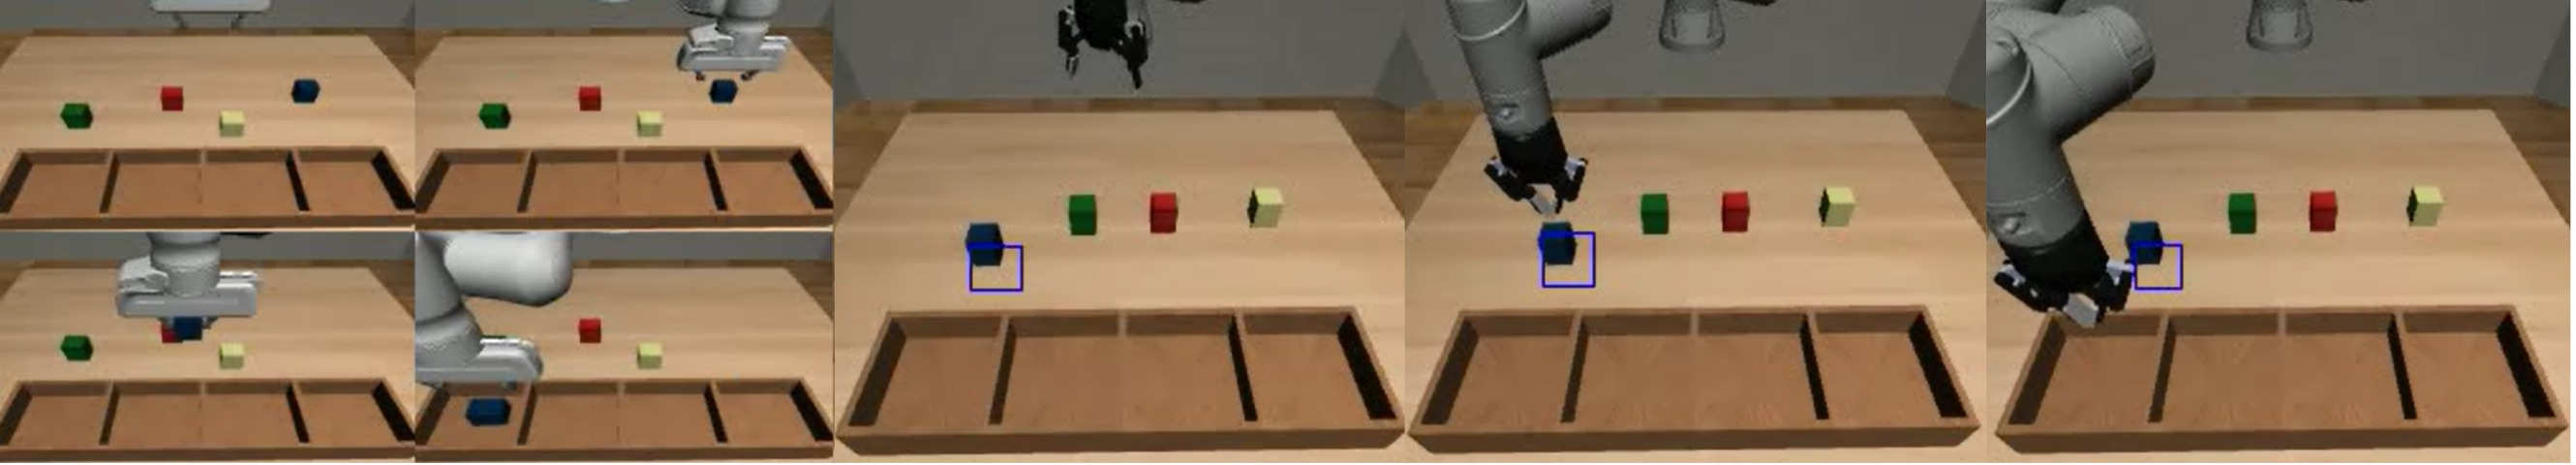
\includegraphics[width=1.0\textwidth]{figures/images/ch3/error_no_bb_after_pick.jpg}
    \caption{Example of an unsuccessful Pick-Place operation using the  ``no-bb after pick" variant. In this scenario, the robot successfully reaches the target box based on the predicted bounding box (blue). However, the single-control module prematurely predicts the closing command, preventing the robot from correctly picking up the object.}
    \label{fig:error_no_bb_after_pick}
\end{figure}

% \smalltodo{add figure}

Regarding the performance of the proposed \textit{MOSAIC-COD} module, it is notable that it achieves the highest success rate in 3 out of 4 tasks. Specifically, for tasks prone to placing the correct object in the wrong position, such as Pick-Place and Nut-Assembly, this type of error is eliminated, resulting in an overall improvement in the success rate.

Additionally, a novel variant of the MOSAIC baseline, \\ \textit{MOSAIC-DP}, has been implemented. This model follows the classic MOSAIC architecture proposed in \cite{mandi2022towards_more_generalizable_one_shot}, but it is equipped with two control modules. One module handles the reaching primitive, while the other is responsible for the primitive used in the final part of the task (i.e., placing, assembly, stacking, or pushing, respectively).

It is important to note that the performance of this variation is very similar to the original MOSAIC baseline, even though the control problem is simplified by splitting it into two phases corresponding to different primitives. Specifically, the most significant error in this case also stems from manipulating the wrong object. The success rates with the wrong object are 54.38\%, 46.67\%, 46.67\%, and 7.59\% for the Pick-Place, Nut-Assembly, Stack-Block, and Press-Button tasks, respectively. 

This further supports the central thesis, which suggests that the end-to-end architecture struggles to create an optimal embedding that addresses both cognitive and control tasks effectively.

\paragraph*{Multi-task multi-variation scenario}\mbox{}\\
\begin{table}[t]
  \scriptsize
  \selectfont
  \centering
  \refstepcounter{table}
  \caption{MOSAIC-COD results obtained in the multi-task setting. The model is compared with MOSAIC and MOSAIC-CTOD models.}
  \label{table:double_policy_multi_task}
  \resizebox{\linewidth}{!}{%
  \begin{tabular}{|c|c|c|c|c|} 
  \hline
  \textbf{Task} & \textbf{Model} & \begin{tabular}[c]{@{}c@{}}\textbf{Reaching}\\{[}\%]\end{tabular} &  \begin{tabular}[c]{@{}c@{}}\textbf{Picking}\\{[}\%]\end{tabular} & \begin{tabular}[c]{@{}c@{}}\textbf{Success}\\{[}\%]\end{tabular} \\ 
  \hhline{|=====|}
  \multirow{3}{*}{Pick-Place} & MOSAIC & 25.83$\pm$1.30 & 23.96$\pm$0.72 & 22.71$\pm$0.72 \\ 
  \cline{2-5}
   & MOSAIC-CTOD & 80.21$\pm$1.44 & 67.50$\pm$0.62 & 53.33$\pm$1.90 \\ 
  \cline{2-5}
   & \textit{MOSAIC-COD} & 100.00$\pm$0.00 & 94.79$\pm$0.90 & \textbf{89.58$\pm$3.55} \\ 
  \hhline{|=====|}
  \multirow{3}{*}{Nut-Assembly} & MOSAIC & 32.96$\pm$1.28 & 30.74$\pm$2.31 & 28.53$\pm$2.31 \\ 
  \cline{2-5}
   & MOSAIC-CTOD & 68.69$\pm$1.11 & 49.63$\pm$3.30 & 33.33$\pm$4.00 \\ 
  \cline{2-5}
   & \textit{MOSAIC-COD} & 99.63$\pm$0.64 & 78.15$\pm$2.31 & \textbf{70.74$\pm$4.49} \\ 
  \hhline{|=====|}
  \multirow{3}{*}{Stack-Block} & MOSAIC & 57.78$\pm$1.92 & 57.78$\pm$1.92 & 55.56$\pm$2.54 \\ 
  \cline{2-5}
   & MOSAIC-CTOD & 97.92$\pm$2.09 & 96.67$\pm$2.35 & \textbf{87.92$\pm$2.00} \\ 
  \cline{2-5}
   & \textit{MOSAIC-COD} & 98.33$\pm$0.00 & 98.33$\pm$0.00 & 85.00$\pm$5.00 \\ 
  \hhline{|=====|}
  \multirow{3}{*}{Press-Button} & MOSAIC & 78.33$\pm$1.66 & - & 77.22$\pm$2.54 \\ 
  \cline{2-5}
   & MOSAIC-CTOD & 92.78$\pm$0.96 & - & \textbf{91.11$\pm$2.54} \\ 
  \cline{2-5}
   & \textit{MOSAIC-COD} & 83.89$\pm$2.55 & - & 71.67$\pm$2.88 \\
  \hline
  \end{tabular}
  }
  \end{table}
Given the results and observations from the previous section, the MOSAIC-COD module is directly compared to the baselines MOSAIC and MOSAIC-CTOD in the Multi-Task setting. Table \ref{table:cod_multi_task_performance} summarizes the results. As can be seen, the use of specialized models trained for the two task phases, reaching and placing, leads to a system that consistently picks the target object. This improvement is particularly evident in the more complex tasks, such as Pick-Place and Nut-Assembly. The enhanced picking rate demonstrates that having accurate information about the target object position enables correct target acquisition, while the presence of two control modules allows for training specific controllers for simpler primitives.

However, despite the improvements observed in Pick-Place and Nut-Assembly, MOSAIC-COD has the lowest overall success rate on the Press-Button task. This can be attributed to two main factors. First, the Press-Button task is substantially different from the other three tasks. Unlike the others, it does not involve pick-and-place primitives, making it an out-of-distribution task. Second, the instability of the bounding boxes produced can lead to undesirable behaviors, such as sudden movements or freezing.
% \smalltodo{add figure}

\subsubsection{Proprioceptive state and Generalization tests}
\begin{figure}[t]
    \centering
    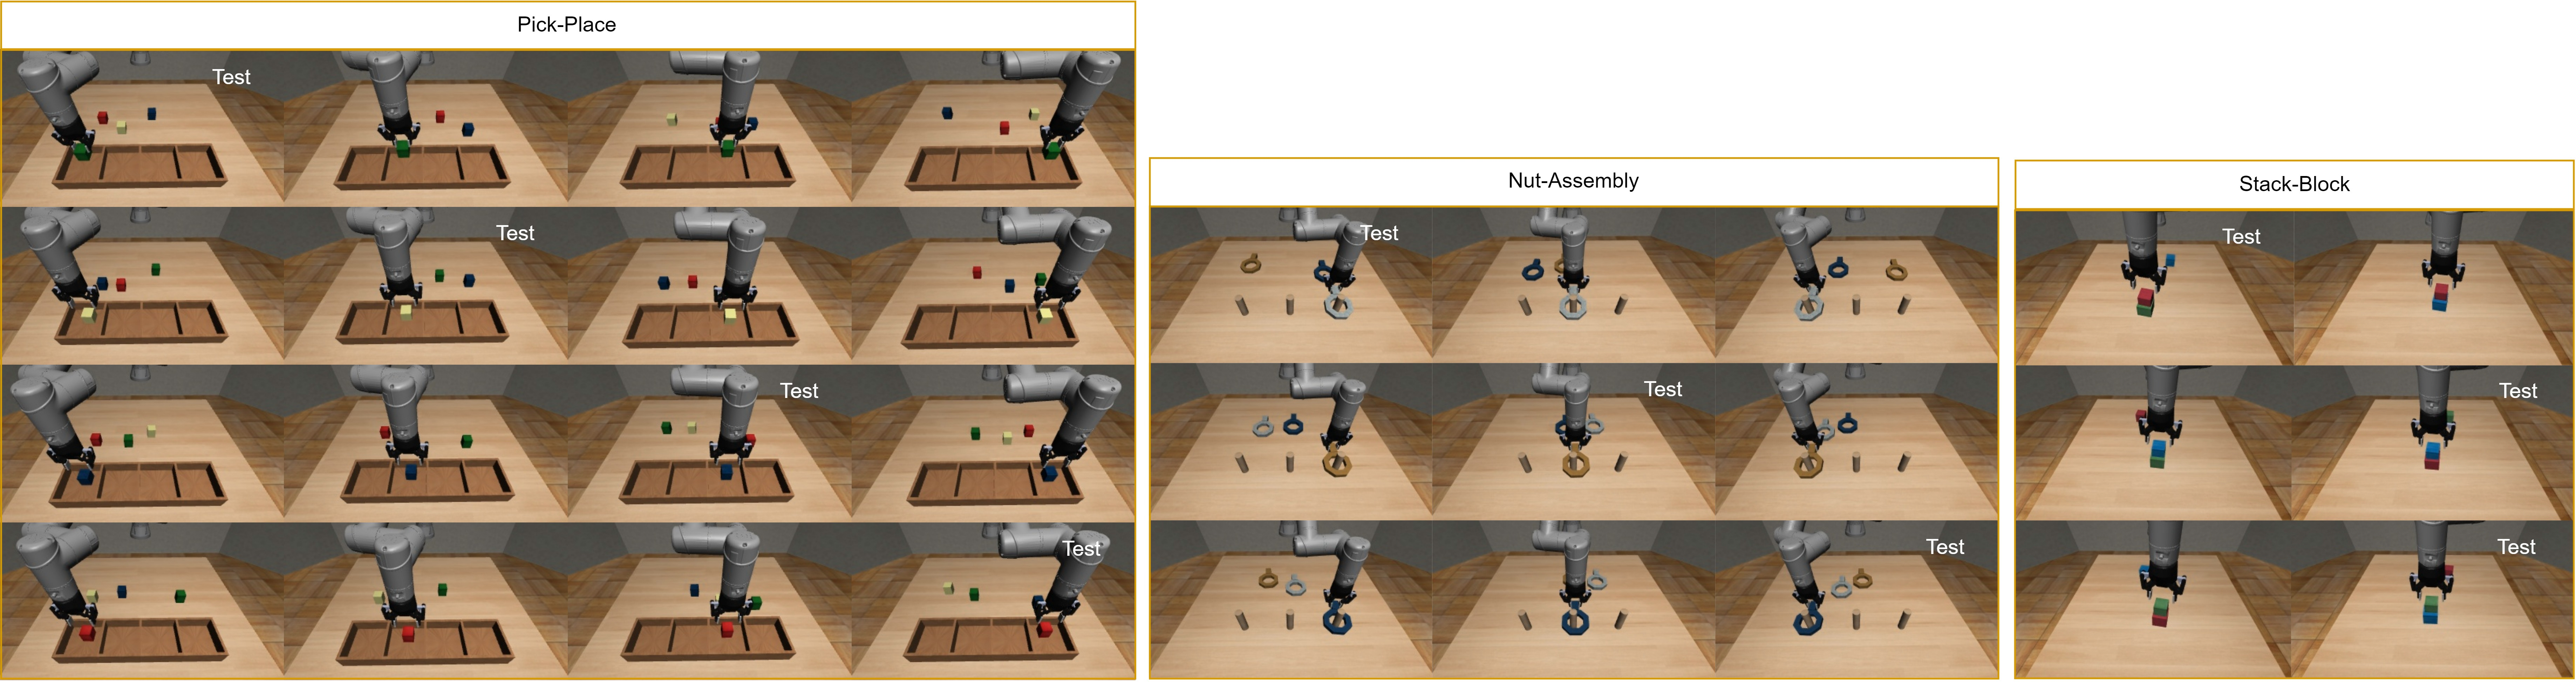
\includegraphics[width=1.0\textwidth]{figures/images/ch3/generalization_dataset.jpg}
    \caption{The dataset used for generalization tests removes one variation from each set of variations for a given target object.}
    \label{fig:generalization_dataset}
\end{figure}


\begin{figure}[t]
    \centering
    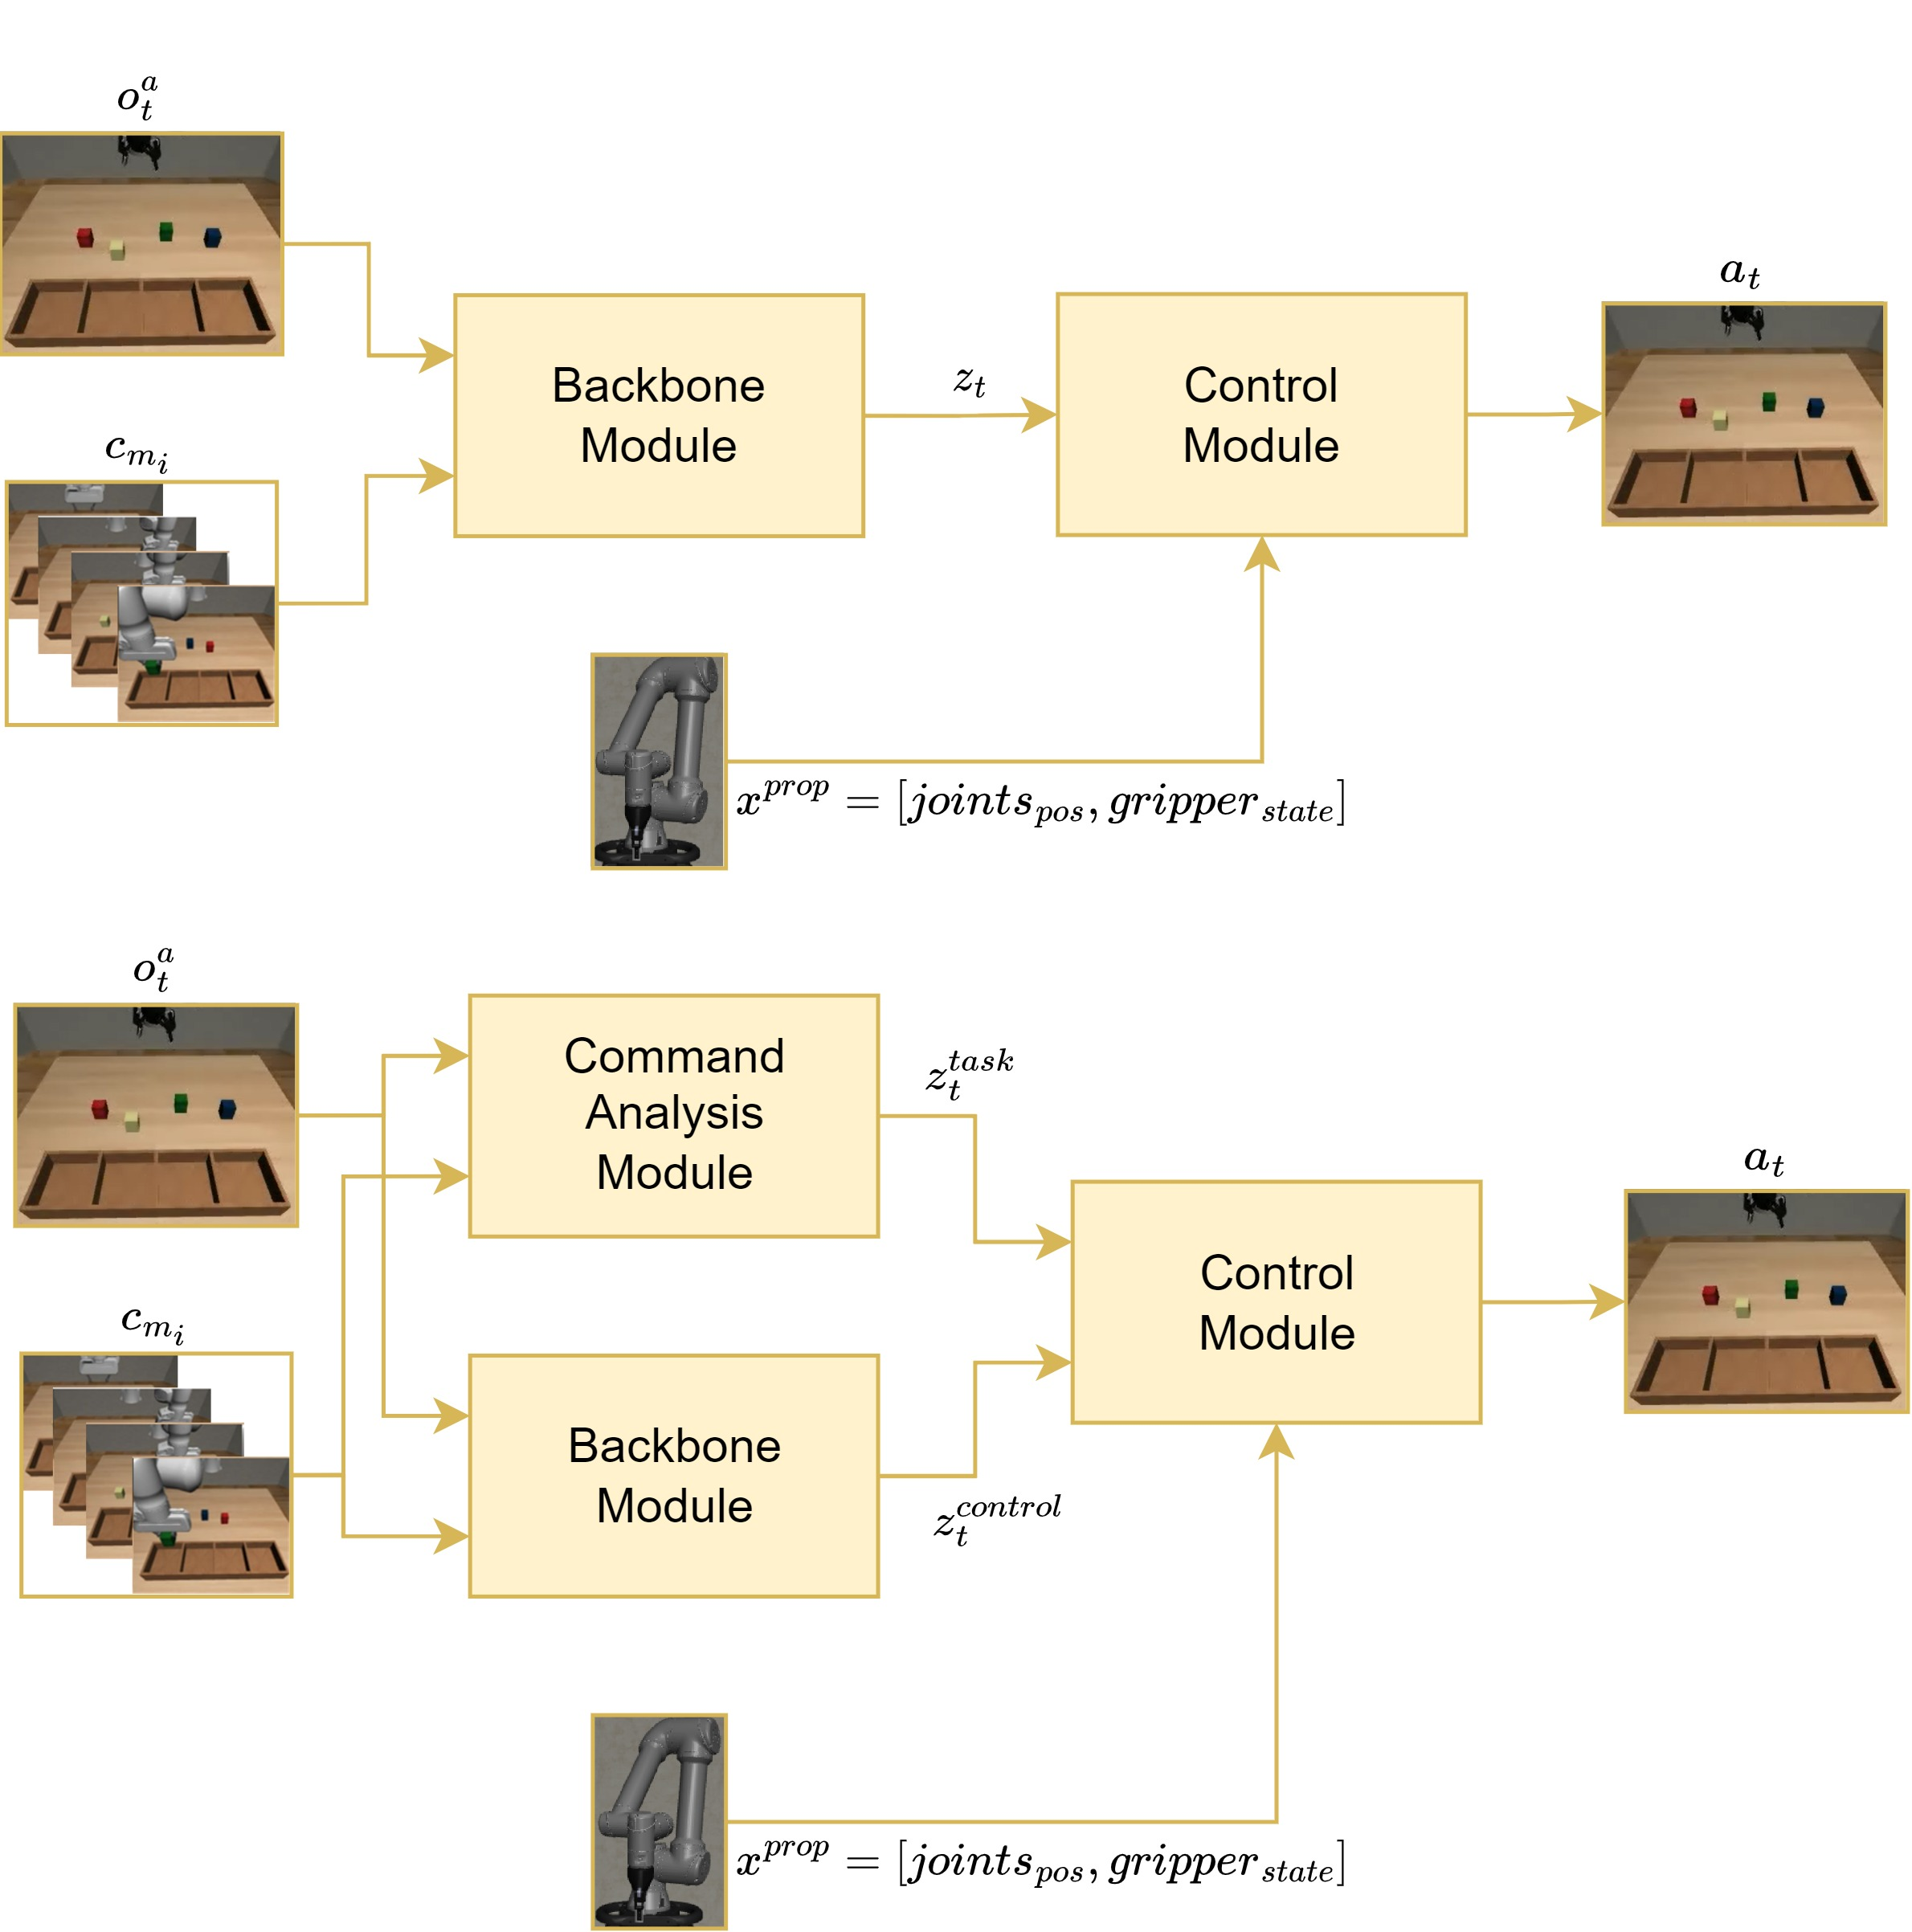
\includegraphics[width=0.7\textwidth]{figures/images/ch3/end_to_end_vs_modular_proprioceptive.jpg}
    \caption{Proprioceptive information is integrated in both the end-to-end architecture (top) and the modular architecture (bottom). The proprioceptive vector, $x^{prop}$, is constructed from the robot's six continuous joint positions and the binary gripper state.}
    \label{fig:end_to_end_vs_modular_proprioceptive}
\end{figure}

In this section, additional experiments are described, focusing on two key objectives.

The first set of experiments aims to determine whether the integration of proprioceptive information can enhance the system's robustness. This is particularly important for tasks requiring fine manipulation, such as the Nut-Assembly task, where the goal is to reduce errors during the assembly phase, specifically avoiding instances where the nut hits the peg.

The second set of experiments explores the generalization capabilities of the proposed system. Specifically, the goal is to assess whether the system can generalize to previously unseen task variations. To evaluate this, the system is trained on a subset of task variations selected as follows: for a set of variations involving a specific target object (e.g., a green box), one variation is excluded (e.g., placing the box into the first bin). However, in other sets involving different objects, the variation that requires placing the object into the first bin is retained. This setup allows for testing how well the system can transfer knowledge across different variations. By doing so, it becomes possible to evaluate whether the system can achieve robust performance with less training data, eliminating the need to collect every possible variation for each object (Figure \ref{fig:generalization_dataset}).
% \smalltodo{add figure}

\begin{table}[t]
  \centering
  \caption{The results obtained by integrating proprioceptive information in both Single-Task and Multi-Task scenarios. For each baseline model, MOSAIC, MOSAIC-CTOD, and MOSAIC-COD, the corresponding version that includes the proprioceptive state (P) was trained and tested.}
  \label{table:proprioceptive}
  \resizebox{\linewidth}{!}{%
  \begin{tabular}{|c|c|c|c|} 
  \hline
  \textbf{Task} & \textbf{Model} & \begin{tabular}[c]{@{}c@{}}\textbf{Success}\\\textbf{(Single-Task)}\\{[}\%]\end{tabular} & \begin{tabular}[c]{@{}c@{}}\textbf{Success}\\\textbf{(Multi-Task)}\\{[}\%]\end{tabular} \\ 
  \hhline{|====|}
  \multirow{6}{*}{Pick-Place} & MOSAIC & 58.75$\pm$1.87 &  \\ 
  \cline{2-4}
   & \textit{MOSAIC-P} & 12.84$\pm$0.31 &  \\ 
  \cline{2-4}
   & MOSAIC-CTOD & 77.11$\pm$5.60 &  \\ 
  \cline{2-4}
   & \textit{MOSAIC-CTOD-P} & 87.84$\pm$2.43 &  \\ 
  \cline{2-4}
   & MOSAIC-COD & 93.33$\pm$0.72 &  \\ 
  \cline{2-4}
   & \textit{MOSAIC-COD-P} & \textbf{96.04$\pm$0.56} &  \\ 
  \hhline{|====|}
  \multirow{6}{*}{Nut-Assembly} & MOSAIC & 33.33$\pm$1.11 &  \\ 
  \cline{2-4}
   & \textit{MOSAIC-P} & 13.83$\pm$0.57 &  \\ 
  \cline{2-4}
   & MOSAIC-CTOD & 64.07$\pm$0.64 &  \\ 
  \cline{2-4}
   & \textit{MOSAIC-CTOD-P} & 95.06$\pm$0.56 &  \\ 
  \cline{2-4}
   & MOSAIC-COD & 81.11$\pm$3.84 &  \\ 
  \cline{2-4}
   & \textit{MOSAIC-COD-P} & \textbf{95.06$\pm$0.57} &  \\ 
  \hhline{|====|}
  \multirow{6}{*}{Stack-Block} & MOSAIC & 53.33$\pm$1.66 &  \\ 
  \cline{2-4}
   & \textit{MOSAIC-P} & 29.07$\pm$2.50 &  \\ 
  \cline{2-4}
   & MOSAIC-CTOD & 91.67$\pm$2.88 &  \\ 
  \cline{2-4}
   & \textit{MOSAIC-CTOD-P} & 91.11$\pm$6.90 &  \\ 
  \cline{2-4}
   & \textit{MOSAIC-COD} & 95.00$\pm$1.66 &  \\ 
  \cline{2-4}
   & \textit{MOSAIC-COD-P} & \textbf{96.67$\pm$1.66} &  \\ 
  \hhline{|====|}
  \multirow{6}{*}{Press-Button} & MOSAIC & \textbf{100.00$\pm$0.00} &  \\ 
  \cline{2-4}
   & \textit{MOSAIC-P} & 65.00$\pm$3.33 &  \\ 
  \cline{2-4}
   & MOSAIC-CTOD & 95.56$\pm$1.92 &  \\ 
  \cline{2-4}
   & \textit{MOSAIC-CTOD-P} & 86.66$\pm$6.66 &  \\ 
  \cline{2-4}
   & MOSAIC-COD & 91.11$\pm$1.92 &  \\ 
  \cline{2-4}
   & \textit{MOSAIC-COD-P} & 72.03$\pm$3.39 &  \\
  \hline
  \end{tabular}
  }
  \end{table}
\paragraph*{Proprioceptive information}\mbox{}\\
The proprioceptive information selected for the four tasks considered includes the joint positions, $joints_{pos} \in \mathcal{R}^{6}$ and the gripper state, $gripper_{state} \in \left[ 0, 1 \right]$. This vector of elements, $x^{prop}$, is provided as input directly to the Control Module, as shown in Figure \ref{fig:end_to_end_vs_modular_proprioceptive}. 
% \smalltodo{add figure}

Specifically, for each baseline method, \textit{MOSAIC}, \textit{MOSAIC-CTOD}, and \textit{MOSAIC-COD}, a version of the model incorporating proprioceptive information was trained. Table \ref{table:proprioceptive} presents the success rates for both the Single-Task and Multi-Task scenarios. 

It is important to note that for 3 out of 4 tasks, the best performance is achieved by combining the Double-Policy approach with proprioceptive information, effectively solving the manipulation tasks of Pick-Place, Nut-Assembly, and Stack-Block in a robust manner. The greatest improvement is seen in the Nut-Assembly task, where the proprioceptive information resolves issues related to collisions and robot freezing.

However, this improvement is not observed in the Press-Button task, where a 35\% drop in success rate is seen, even with the \textit{MOSAIC} baseline. In this task, the main failure cases are related to unstable robot behavior. Additionally, in variations focused on object orientation, the robot often gets stuck when correctly approaching the button.

Notably, this behavior is not observed in the Multi-Task scenario. In fact, the highest performance is achieved by methods that exclude proprioceptive information. Interestingly, the inclusion of proprioceptive data seems to exacerbate the imbalance between tasks, preventing the system from effectively leveraging this additional information during testing and resulting in instability.

For example, in the case of the MOSAIC-CTOD-P module, the robot successfully picks the target object only 58.87\% of the time. This occurs because the closing command is sent too early, relative to the object position. Furthermore, the success rate drops further to 38.14\%, as the robot, despite reaching the target peg, collides with it, an issue where proprioceptive information should theoretically provide assistance, especially since the pegs are fixed.

This instability is most evident in the Stack-Block task, where the success rate falls to 22.77\% for the MOSAIC-COD-P module, despite the robot picking the target object with an average rate of 80.00\%. The errors in this case are due to the object being dropped during stacking, caused by imprecise placement, as well as instances where the robot becomes completely stuck.

These results highlight the need for a balanced learning procedure in the context of Multi-Task Learning, as discussed earlier in Section \ref{sec:ocpl_results_scm}.

% \usepackage{graphicx}
% \usepackage{multirow}
% \usepackage{hhline}


\begin{table}[t]
  \centering
  \caption{The results obtained by testing the models on unseen variations.}
  \label{table:generalization}
  \resizebox{\linewidth}{!}{%
  \begin{tabular}{|c|c|c|c|c|c|} 
  \hline
  \textbf{Task} & \textbf{Model} & \begin{tabular}[c]{@{}c@{}}\textbf{Reaching}\\\textbf{(Single-Task)}\\{[}\%]\end{tabular} & \begin{tabular}[c]{@{}c@{}}\textbf{Success}\\\textbf{(Single-Task)}\\{[}\%]\end{tabular} & \begin{tabular}[c]{@{}c@{}}\textbf{Reaching}\\\textbf{(Multi-Task)}\\{[}\%]\end{tabular} & \begin{tabular}[c]{@{}c@{}}\textbf{Success}\\\textbf{(Multi-Task)}\\\textbf{\textbf{}}\%]\end{tabular} \\ 
  \hhline{|======|}
  \multirow{3}{*}{\vspace{-30px}\rotatebox[origin=c]{90}{Pick-Place}} & MOSAIC & 35.83$\pm$2.82 & 31.67$\pm$3.82 & 32.50$\pm$2.50 & 20.83$\pm$5.70 \\ 
  \cline{2-6}
   & \begin{tabular}[c]{@{}c@{}}\textbf{\textit{MOSAIC-CTOD}}\\\textbf{\textit{(proposal)}}\end{tabular} & 100.00$\pm$0.00 & 87.50$\pm$4.30 & 100.00$\pm$0.00 & 63.33$\pm$5.20 \\ 
  \cline{2-6}
   & \begin{tabular}[c]{@{}c@{}}\textbf{\textit{MOSAIC-COD}}\\\textbf{\textit{(proposal)}}\end{tabular} & 100.00$\pm$0.00 & \textbf{89.17$\pm$2.89} & 100.00$\pm$0.00 & \textbf{94.17$\pm$2.88} \\ 
  \hhline{|======|}
  \multirow{3}{*}{\vspace{-30px}\rotatebox[origin=c]{90}{Nut-Assembly}} & MOSAIC & 22.22$\pm$1.93 & 13.33$\pm$3.33 & 27.78$\pm$3.85 & 18.88$\pm$3.84 \\ 
  \cline{2-6}
   & \begin{tabular}[c]{@{}c@{}}\textbf{\textit{MOSAIC-CTOD}}\\\textbf{\textit{(proposal)}}\end{tabular} & 100.00$\pm$0.00 & 38.89$\pm$6.94 & 100.00$\pm$0.00 & 51.11$\pm$1.92 \\ 
  \cline{2-6}
   & \begin{tabular}[c]{@{}c@{}}\textbf{\textit{MOSAIC-COD}}\\\textbf{\textit{(proposal)}}\end{tabular} & 98.89$\pm$1.93 & \textbf{57.78$\pm$5.09} & 100.00$\pm$0.00 & \textbf{90.00$\pm$3.33} \\ 
  \hhline{|======|}
  \multirow{3}{*}{\vspace{-30px}\rotatebox[origin=c]{90}{Stack-Block}} & MOSAIC & 58.89$\pm$1.93 & 53.33$\pm$3.33 & 60.00$\pm$5.77 & 56.66$\pm$3.33 \\ 
  \cline{2-6}
   & \begin{tabular}[c]{@{}c@{}}\textbf{\textit{MOSAIC-CTOD}}\\\textbf{\textit{(proposal)}}\end{tabular} & 100.00$\pm$0.00 & 94.44$\pm$6.94 & 100.00$\pm$0.00 & \textbf{88.88$\pm$5.00} \\ 
  \cline{2-6}
   & \begin{tabular}[c]{@{}c@{}}\textbf{\textit{MOSAIC-COD}}\\\textbf{\textit{(proposal)}}\end{tabular} & 100.00$\pm$0.00 & \textbf{97.78$\pm$1.93} & 100.00$\pm$0.00 & 72.20$\pm$5.09 \\
  \hline
  \end{tabular}
  }
  \end{table}
\paragraph*{Generalization}\mbox{}\\
Regarding the generalization tests, we evaluated only the three tasks where the previously explained variation selection was applicable. Specifically, the following variations were removed for each task (Figure \ref{fig:generalization_dataset}):

\begin{itemize}
    \item \textbf{Pick-Place}: Variations 1, 6, 11, and 16 were excluded.
    \item \textbf{Nut-Assembly}: Variations 1, 5, and 9 were excluded.
    \item \textbf{Stack-Block}: Variations 1, 4, and 6 were excluded.
\end{itemize}

The models were trained on the remaining variations and tested on the excluded ones following the same procedure.

Table \ref{table:generalization} summarizes the success rates obtained for both the Single-Task and Multi-Task settings. Notably, with the introduction of the CTOD and COD modules, the system consistently reaches the correct target object in unseen variations. Similarly, the robot is able to pick and complete tasks, outperforming the MOSAIC baseline across all tested tasks.

This is a promising result, as it demonstrates that the system can effectively share knowledge across different variations, enabling robust training with fewer data.




\section{Conclusion}
In conclusion, this chapter introduced and discussed the Object Conditioned Control Policy (OCCP), a modular control architecture designed to integrate the Conditioned Object Detector. This integration allows the control policy to utilize low-dimensional positional information about the target object location, while the Control Module Backbone generates an embedding containing task-relevant information. This embedding is derived from gradients obtained through the backpropagation of an action-centric loss function, thereby addressing or mitigating the target-object misidentification issues observed in baseline models.

Two specific control architectures were proposed: MOSAIC-CTOD, which integrates the Conditioned Target Object Detector, and MOSAIC-COD, which incorporates the Conditioned Object Detector. The latter generates both the bounding box of the target object and the bounding box of the target position of interest.

These architectures were validated in a simulation environment under both single-task multi-variation and multi-task multi-variation scenarios. Results demonstrated that incorporating object-related information enabled the system to consistently reach and pick the target object, leading to successful task completion.

In the single-task scenario, MOSAIC-COD achieved the highest average success rate (\textbf{90.13\%}), representing a $+28.77\%$ improvement over the MOSAIC baseline. In the multi-task scenario, MOSAIC-COD achieved an average success rate of \textbf{79.24\%}, improving by $+33.23\%$ compared to the baseline. The most significant improvements from object conditioning were observed in tasks involving ``pick-place" primitives, such as Pick-Place, Nut-Assembly, and Stack-Block. However, a general performance drop was noted in the Press-Button task, where variations in bounding-box predictions led to unstable robot behaviors.

Additional notable improvements were observed when proprioceptive information (e.g., joint positions and gripper state) was integrated. Specifically, the Nut-Assembly task, which requires precise, contact-rich manipulation, saw the highest gains. For MOSAIC-CTOD-P, the average success rate reached \textbf{95.06\%}, marking an improvement of $+30.99\%$ over the version without proprioceptive data. This success was attributed to the fixed positions of the target pegs, where joint position information helped the robot avoid collisions and correctly insert the pegs.

Moreover, the proposed architecture demonstrated zero-shot generalization to novel variations, with MOSAIC-COD achieving an average success rate of \textbf{81.57\%} in the single-task scenario and \textbf{85.45\%} in the multi-task scenario. This represents improvements of $+48.79\%$ and $+53.32\%$ over the MOSAIC baseline, respectively.

Overall, the introduction of inferred object priors led to significant improvements over the baseline. However, further refinements in the learning process, particularly in multi-task scenarios, are needed. Specifically, future work should account for the varying difficulties of different tasks in these scenarios.